% Document class
\documentclass{article}

% Packages
\usepackage[utf8]{inputenc}
\usepackage[english]{babel}
\usepackage{mathtools}
\usepackage{gensymb}
\usepackage{amstext}
\usepackage{amsmath}
\usepackage{graphicx}
\usepackage{textcomp}
\usepackage{float}
\usepackage{varioref}
\usepackage{fancyref}
\usepackage{caption}
\usepackage{subcaption}
\usepackage{comment}
\usepackage{hyperref}
\usepackage{epstopdf}
\usepackage[margin=1in, paperwidth=8.5in, paperheight=11in]{geometry}
\usepackage{gensymb}
\usepackage{listings}
\usepackage{xcolor}
\usepackage{listings}
\usepackage{pdfpages}
\usepackage{graphicx}
\usepackage{wrapfig}
\usepackage{lscape}
\usepackage{rotating}
\usepackage{epstopdf}
\usepackage{fancyhdr}
\usepackage{amssymb}
\usepackage{fancyhdr}
\usepackage{soul}

\graphicspath{{images/}}

\usepackage{helvet} %font
% Document Setup
\pagenumbering{roman}
\pagestyle{fancy}

\addto\captionsenglish{\renewcommand*\contentsname{Table of Contents}}

\DeclareRobustCommand{\hlr}[1]{{\sethlcolor{red}\hl{#1}}}

\begin{document}


\renewcommand{\headrulewidth}{0pt}
\lhead{Olin College of Engineering, E218}
\chead{}
\rhead{\rightmark}
\lfoot{2016 Formula SAE Electric}
\cfoot{
\includegraphics[width=2cm]{revo.png}}
\rfoot{\thepage}

\begin{titlepage}

    \centering
    \vfill
    
\includegraphics[width=10cm]{revo.png}

    {\bfseries\Large
        REVO Electric Racing, Olin College of Engineering\\
        \vskip2cm
        Electrical System Form FSAE-E 2016\\
        Car \hlr{E218}\\
    }

    \begin{table}[H]
        \centering
        \label{my-label}
        \begin{tabular}{lr}
        University Name: & Olin College of Engineering \\ \hline
        Team Name: & REVO Electric Racing \\ \hline
        Car Number: & \hlr{E218} \\ \hline
        ESF Contact: & Lisa Hachmann \\ \hline
        e-mail: & Lisa.Hachmann@students.olin.edu \\ \hline
        \end{tabular}
    \end{table}
\vfill

\begin{figure}[H]
\centering
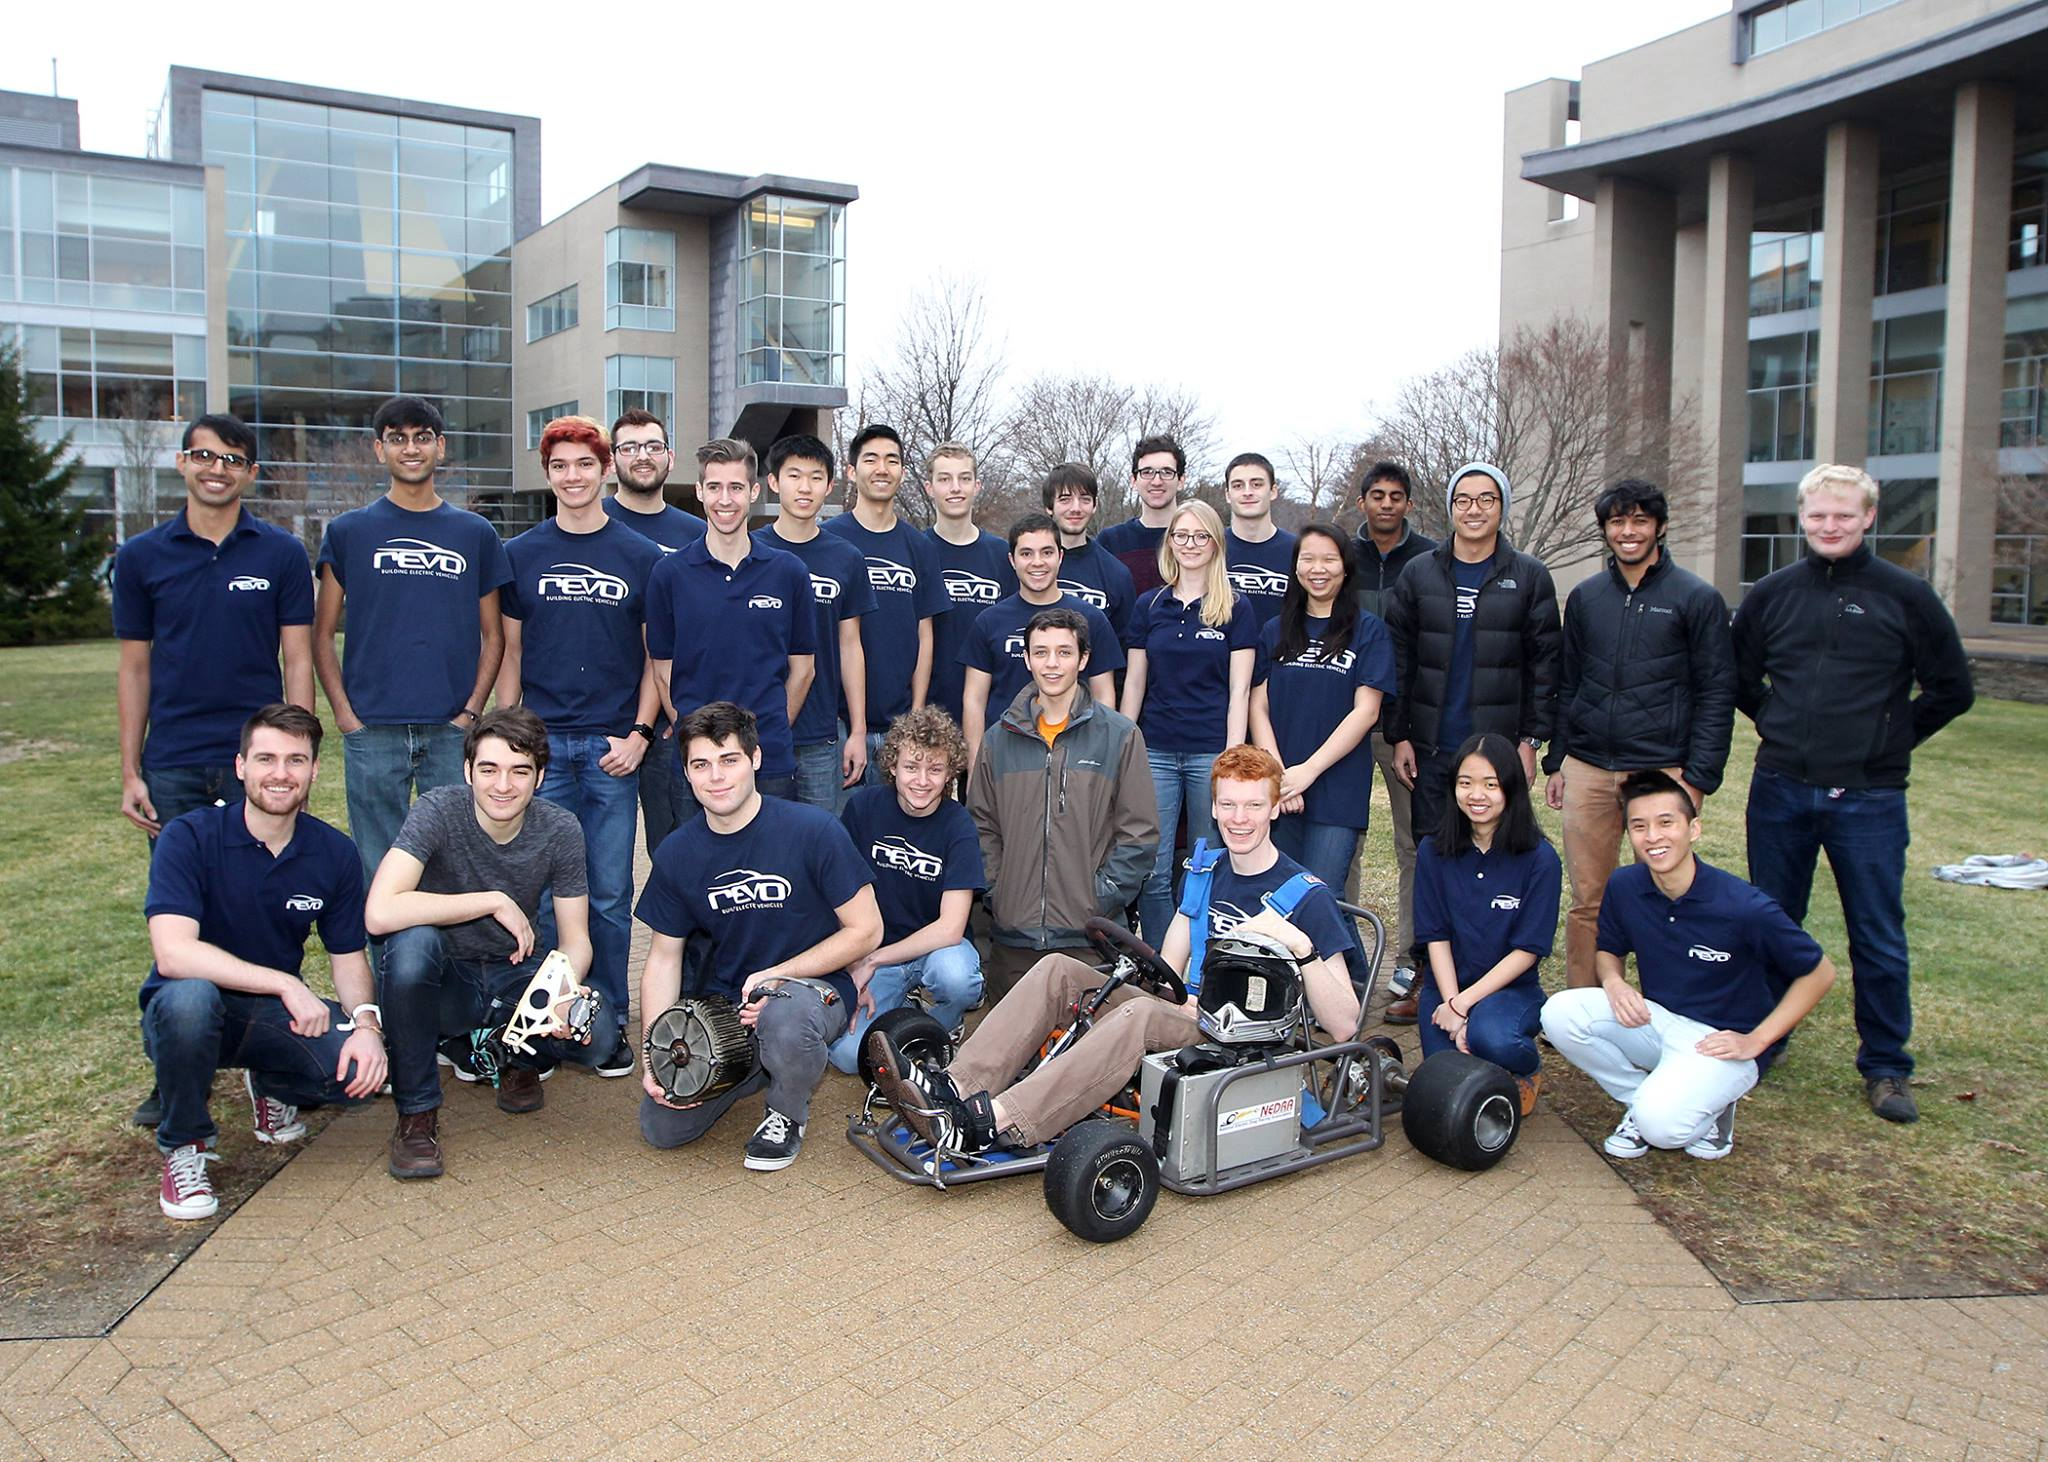
\includegraphics[width = 0.9 \textwidth]{teamPhoto}
\end{figure}

\end{titlepage}


\tableofcontents
\addcontentsline{toc}{section}{Table of Contents}

\newpage
\listoffigures
\addcontentsline{toc}{section}{List of Figures}

\newpage
\listoftables
\addcontentsline{toc}{section}{List of Tables}

\newpage
\section*{List of Abbreviations}
\addcontentsline{toc}{section}{List of Abbreviations}
\begin{itemize}
    \item MSD- Manual Service Disconnect
    \item CONN- Main accumulator connector
    \item \hlr{NDA - Non Disclosure Agreement}
    \item \hlr{SDB- Shutdown Button}
\end{itemize}


    Any other abbreviations used in this document are those used in the 2016 Formula SAE Rules and those used in the FSAE ESF template document.

\setlength{\parindent}{0pt}

\newpage
\pagenumbering{arabic}


\section{System Overview} %Short description of system's concept

    The system will support all requirements for vehicular movement while guaranteeing driver and maintenance safety. There will be two primary electrical systems, galvanically isolated from each other: a 100V high power tractive system and a 12V low power sense and communication system.\\

    The low power system will include a shutdown circuit, a series of sensors and switches that ensures the vehicle is safe to drive before engaging the tractive system. \hlr{There is a low voltage battery and DC-DC converter, because the 12V battery will start up the car and the DC-DC converter will take over and continue powering the system (the DC-DC converter being before the AIRs).} The shutdown circuit will monitor the vehicle for dangerous conditions, such as a collision or ground fault in the tractive system, and will disengage the tractive system in case of emergency. Finally, the low power system will power a CAN communication network using ATmega16M1 microcontrollers that will be used to operate several rules required functions, such as the ready to drive sound, but will also serve as a debugging tool for both electrical systems.\\

    \hlr{The tractive system consists of a custom accumulator container, two Sevcon motor controllers, and two Zero Motorcycles brushless DC motors.} The accumulator comprises 12 Nissan Leaf battery modules. The motors are configured for rear wheel drive with independent control over the left and right wheels. Communication to the motor controllers is completed using \hlr{an analog signal from the isolated CAN system.}\\

    See Figure \ref{tractive} for an electrical block diagram.

        \begin{sidewaysfigure}[p]
            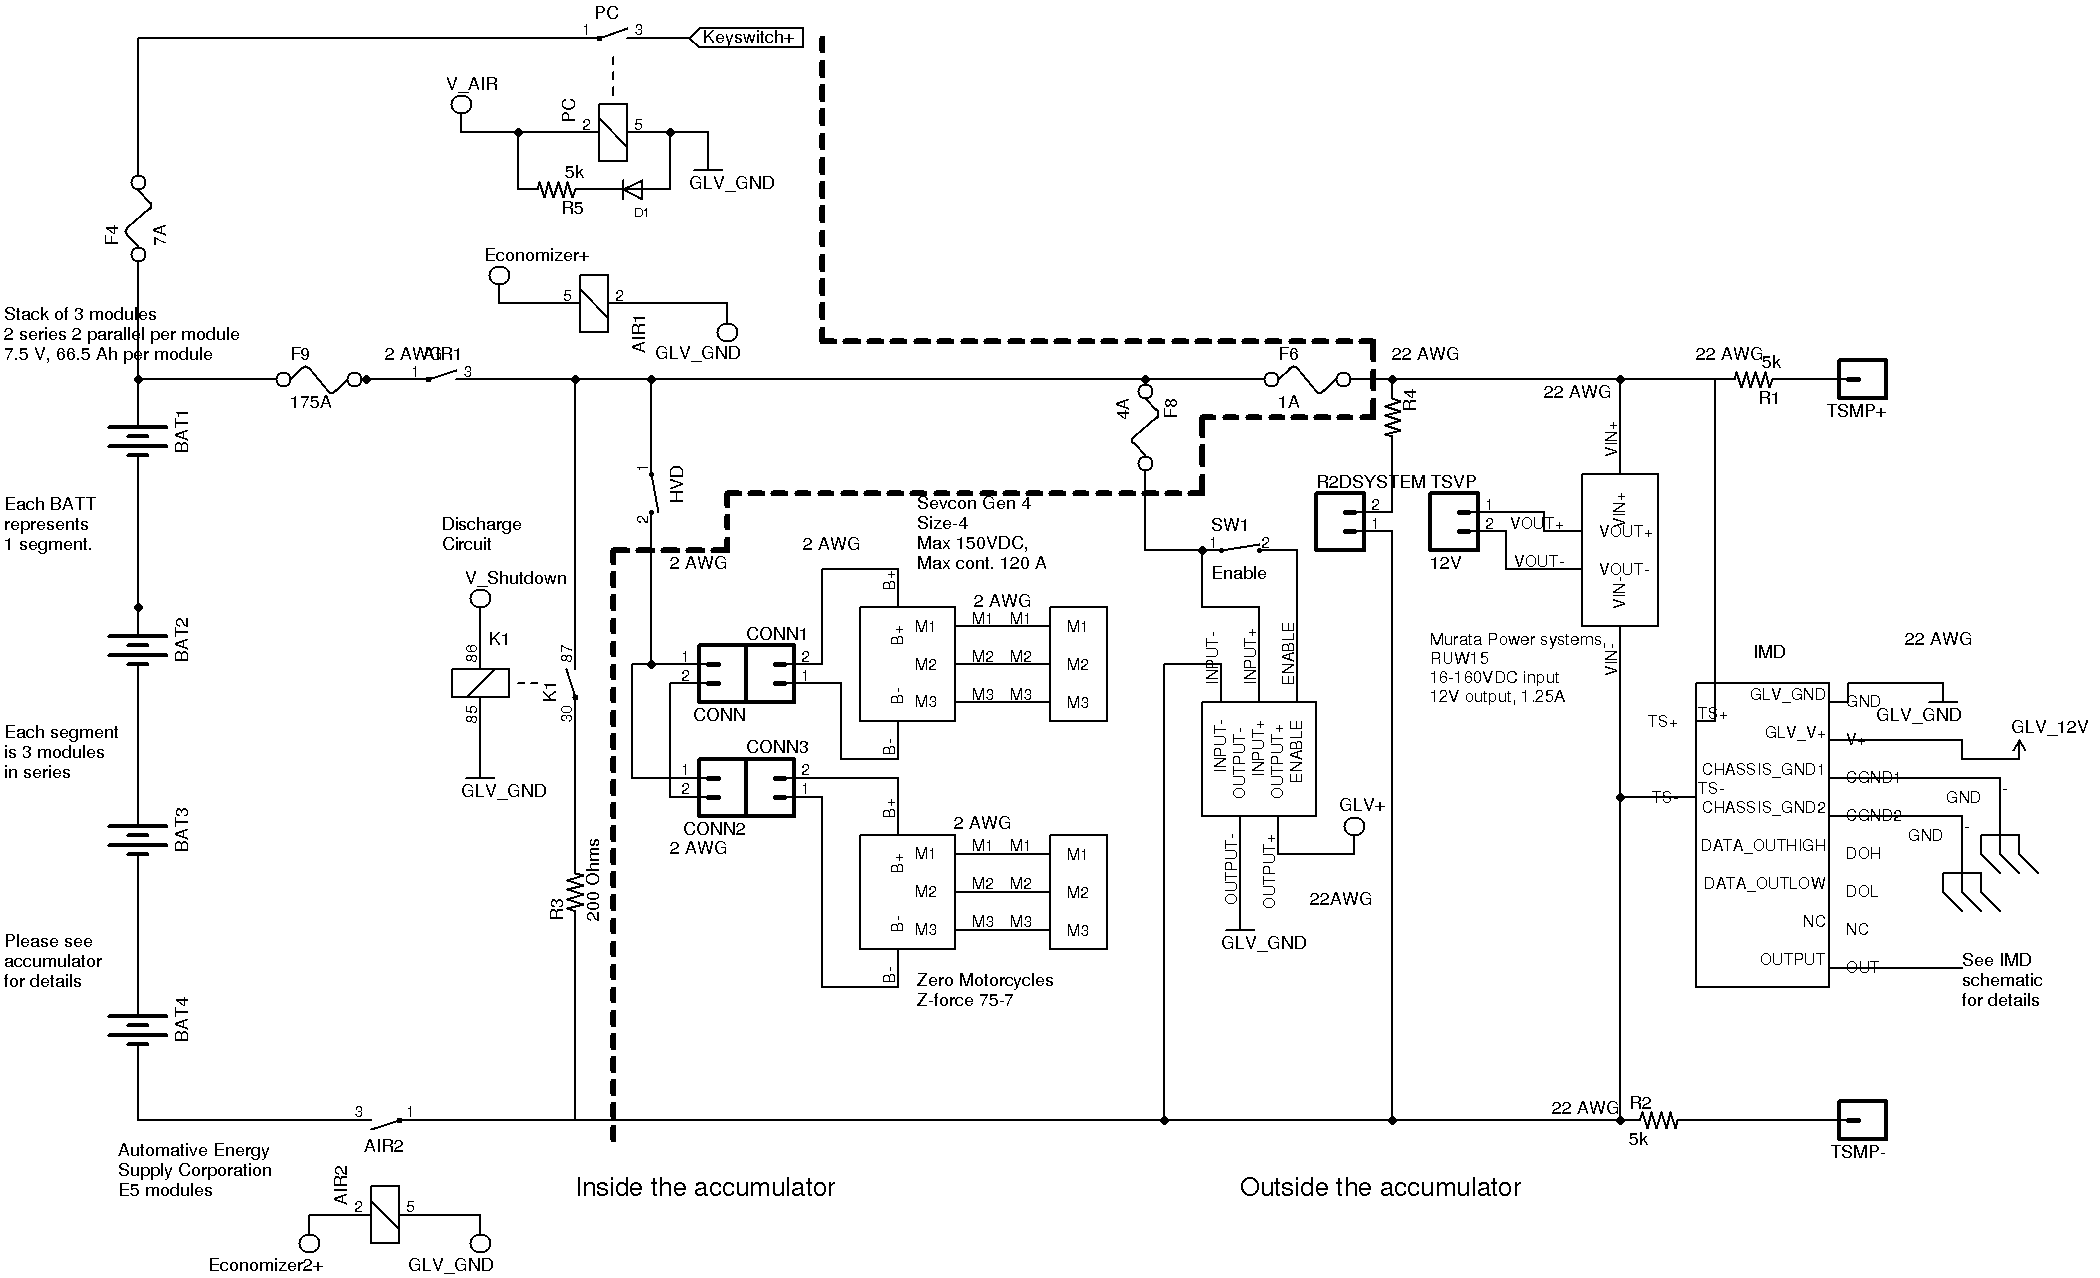
\includegraphics[width=\textheight]{tractiveblock}
            \caption{\hlr{Tractive system block diagram}}
            \label{tractive}
        \end{sidewaysfigure}

        \begin{table}[H]
            \centering
            \begin{tabular}{|l|l|}
            \hline
                Maximum Tractive system voltage & 99.6V VDC \\ \hline
                Nominal Tractive system voltage & 90 VDC \\ \hline
                Control-system voltage & 13.5VDC \hlr{\& 12VDC}\\ \hline
                Accumulator configuration & 2s2p in 12s \\ \hline
                Total Accumulator capacity & \hlr{65.0} \\ \hline
                Motor type & Brushless DC Motor \\ \hline
                Number of motors & Total: 2 \\ \hline
                Maximum combined motor power in kW & 65.7 kW \\ \hline
            \end{tabular}
            \caption{General parameters}
            \label{systemtable}
        \end{table}

\newpage

\section{Electrical Systems}

    \subsection{Shutdown Circuit}

        \subsubsection{Description/Concept}

            The shutdown circuit is the primary method for maintaining driver and maintenance electrical safety at all times. The shutdown circuit prevents high voltage from being present outside of the accumulator container before the vehicle is safe to drive and will shut down the tractive system during driving if it detects an unsafe or emergency condition. The shutdown circuitry \hlr{directly controls the current going to the AIRs through a series of safety sensors and relays}. Triggering the shutdown circuit opens the circuit and causes the AIRs to open. \hlr{To power the system, we have both a DC-DC converter and a 12V 0.8Ah lead acid battery. The battery allows the vehicle to start and the GLV system to power up the TS system. Then, the DC-DC converter powers the car for the rest of the functional time. The battery is left there for backup purposes. }\\

            The shutdown circuit consists of 10 major components

                \begin{itemize}
                    \item The GLVMS controls all power to the GLV system. As a result, high voltage cannot be present when the low voltage system is not active.
                    \item The TSMS is the last component in the shutdown circuit before the AIRs. This allows full testing of the GLV system without engaging the TS and only intentional use of the TS.
                    \item The BOTS is used to detect a mechanical failure in the brake system. If the brake \hlr{system} fails, the TS is disabled to allow the vehicle to roll to a stop and ensure the safety of the driver.
                    \item The SDBs are used for emergency shutdown of the TS. The cockpit SDB allows the driver to quickly shutdown the \hlr{tractive system} from the driver's seat. The left and right SDBs are intended for emergency shutdown in a crash or rollover scenario by first responders.
                    \item The IMD is used to detect if the TS \hlr{has lost isolation with the GLV system}. Because the chassis is used to ground the GLVS, \hlr{lost isolation} presents a dangerous driver and maintenance scenario so the IMD disables the TS.
                    \item The AMS monitors the \hlr{state} of the accumulator and triggers a TS shutdown if the modules enter a dangerous temperature or electrical condition.
                    \item The inertia switch triggers a TS shutdown if it experiences an acceleration indicative of a collision. This ensures the vehicle is electrically safe in an emergency situation.
                    \item Interlocks close the shutdown circuit when all high voltage connections are properly made. This ensures that high voltage is only present within the TS and disabled if connections are left open.
                    \item The BSPD detects if the motor controllers are drawing significant current from the accumulator while the brakes are engaged. To protect the driver and the vehicle, this scenario triggers a TS shutdown.
                    \item Finally, the shutdown circuit contains a CAN Watchdog to shut down the TS in the event of a CAN error. The primary intent of this additional component is to monitor the health of the motor controllers and shutdown TS if necessary to protect them.
                \end{itemize}

            %Describe concept, the master switches, bots, and fill table
            %add additional switches in the table

            \begin{table}[H]
                \centering
                \begin{tabular}{|l|l|}
                \hline
                    Part & Function \\ \hline
                    Main Switch (GLVMS and TSMS) & Normally open \\ \hline
                    Brake over travel switch (BOTS) & \hlr{Push-pull button} \\ \hline
                    Shutdown buttons (SDB) (Left, right, cockpit) & Normally closed \\ \hline
                    Insulation Monitoring Device (IMD) & Normally open \\ \hline
                    Battery Management System  (AMS) x4 & Normally open \\ \hline
                    Inertia switch & Normally closed \\ \hline
                    Interlocks & Closed when circuits are connected \\ \hline
                    Brake System Plausibility Device (BSPD) & Normally Open \\ \hline
                    CAN Watchdog & Normally closed \\ \hline
                \end{tabular}
                \caption{List of switches in the shutdown circuit}
                \label{switchlist}
            \end{table}

        \subsubsection{Wiring/Additional Circuitry}

            %Describe wiring and additional circuitry, show extra schematics if you do something weird, then describe the additional circuitry and use a lot of figures

            \begin{figure}[H]
                \centering
                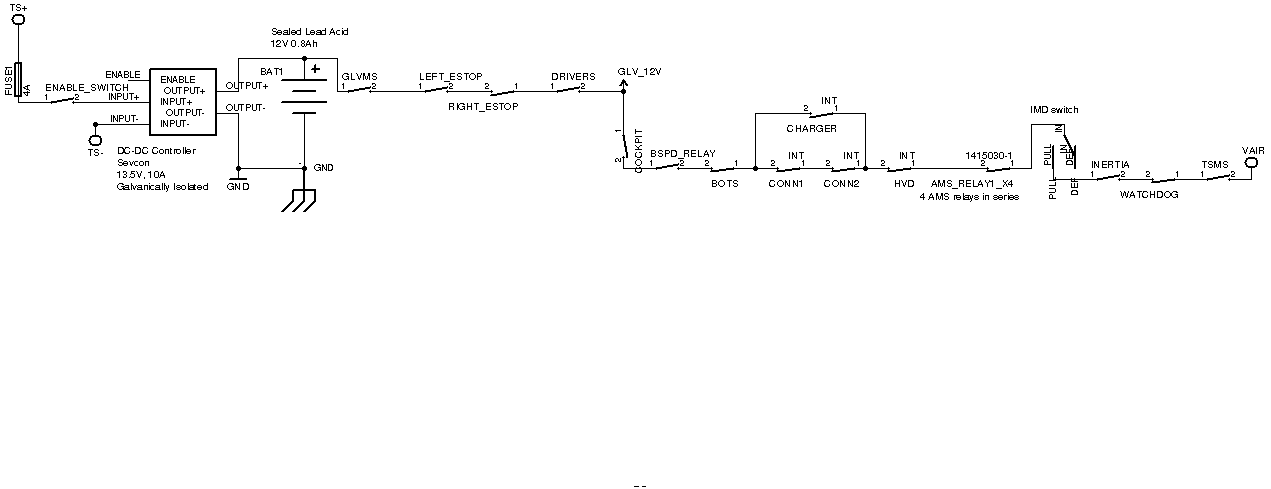
\includegraphics[width = 1 \textwidth]{shutdownswitches}
                \caption{\hlr{Shutdown Circuit Switches}}
                \label{switchesonly}
            \end{figure}

            Figure \ref{switchesonly} shows only the switches in the shutdown circuit, and does not include the AIRs or the precharge and discharge systems. The tractive system can only be enabled when all switches are closed, allowing the AIRS to be closed. The point after the TSMS splits into power for the AIRs, which are in parallel, the keyswitch (trigger for the internal precharge system of the motor controller) \hlr{and the discharge system}. This schematic has been simplified to not include the circuitry around the coils that close these switches, but those schematics can be found in their respective sections.

            \begin{table}[H]
                \centering
                \begin{tabular}{|l|l|}
                \hline
                    Total Number of AIRs: & 2 \\ \hline
                    Current per AIR & \hlr{ 3.8A until 150 ms passes, then 0.4 A} \\ \hline
                    Additional parts consumption within the shutdown circuit: & \hlr{0.5 A }\\ \hline
                    Total current: & \hlr{4.3 A until 150 ms passes, then ~1A} \\ \hline
                    Cross sectional area of the wiring used: & 0.000506 in$^{2}$ (22 AWG) \\ \hline
                \end{tabular}
                \caption{Wiring--Shutdown Circuit}
                \label{ShutdownCircuitTable}
            \end{table}

            The GLV system also has 12V and 5V supply lines in parallel to the shutdown circuit. It supplies the 555 timers, CAN nodes, coils and lights, \hlr{ which are all in parallel with the AIRs, increasing the total current to 1A. }

        \subsubsection{Position in Car}

        \hlr{With the exception of the emergency shutdown buttons and tractive system interlocks, the components comprising the shutdown circuit are housed within a waterproof enclosure, located at the rear of the chassis, behind the main hoop, on the driver's right.  This enclosure is bolted onto steel brackets which are welded to the main hoop.  This enclosure consists of an ABS panel where the TSMS, GLVMS, TSMPs, GLVMPs, AMS, and IMD reset will be mounted, and a 3D printed rear housing with integrated 23-pin Deutsch DT panel mount connector, as seen in figure} \ref{cpanel1}. \hlr{In addition to the buttons and measuring points, the housing also contains the IMD, IMD relay, a PCB, a DC-DC converter, and an SLA battery, as seen in figure} \ref{cpanel2}.  \hlr{The tractive system and low voltage systems are separated by at least two centimeters at all times.}

            \begin{figure}[H]
                \centering
                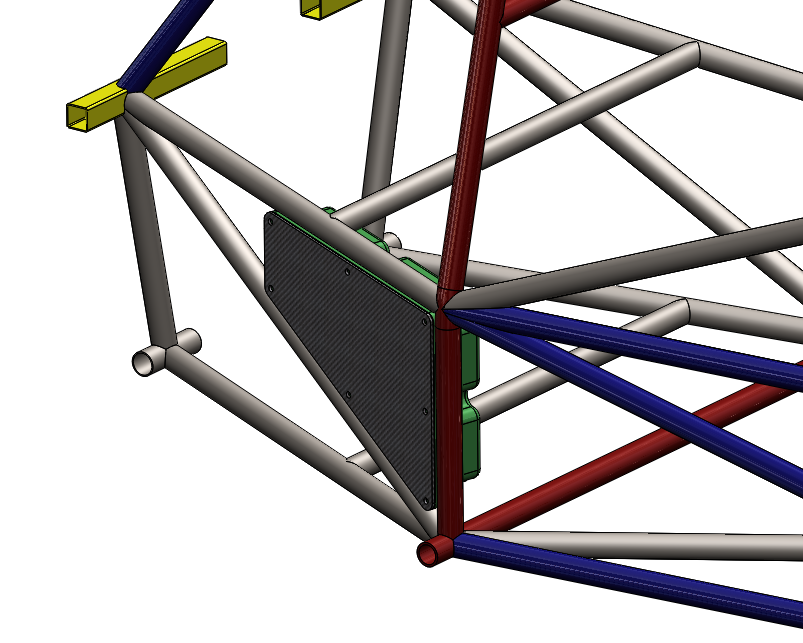
\includegraphics[width = 0.6 \textwidth]{CONTROLPANEL_1}
                \caption{\hlr{Shutdown Circuit Enclosure Vehicle Location}}
                \label{cpanel1}
            \end{figure}

            \begin{figure}[H]
                \centering
                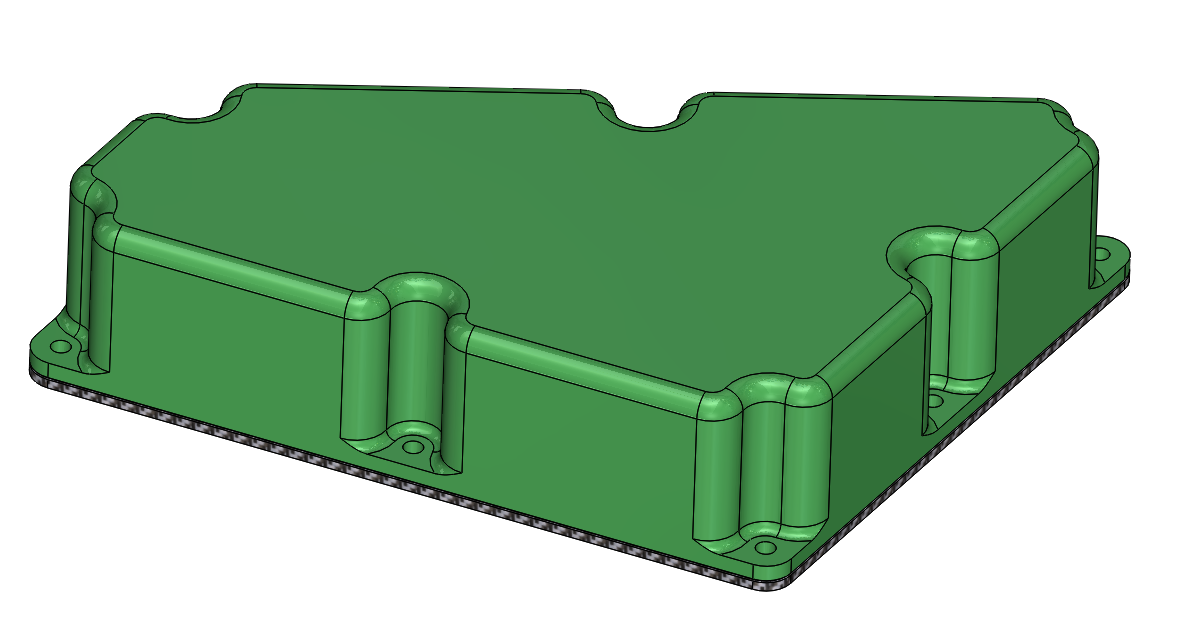
\includegraphics[width = 0.6 \textwidth]{CONTROLPANEL_2}
                \caption{\hlr{Waterproof Enclosure for TS MS, GLV MS, TSMP, GLVMP, \& Shutdown Circuit}}
                \label{cpanel2}
            \end{figure}

    \subsection{IMD}

        \subsubsection{Description (Type, Operation Parameters)}

            The IMD used will be a Bender A-ISOMETER \hlr{IR155-3204}. \hlr{The output is normally high and only low} if it does not detect a ground fault. The output is then used in a \hlr{4PDT} relay to \hlr{close} the switch in the shutdown circuit \hlr{and activate the CAN system to not power the IMD light in the dashboard}.
            %Need to include set point of ground fault

            \begin{table}[H]
                \centering
                \begin{tabular}{|l|l|}
                \hline
                    Supply voltage range: & 10...36VDC \\ \hline
                    Supply voltage & 12VDC \\ \hline
                    Environmental temperature range: & Unknown \\ \hline
                    Selftest interval: & Every 5 minutes \\ \hline
                    High voltage range: & 0-1000 VDC \\ \hline
                    Set response value: & 100 k\ohm\\ \hline
                    Max. operation current: & 150 mA \\ \hline
                    Approximate time to shut down at 50$\%$ of the response value: & $\leq$ 40 sec \\ \hline
                \end{tabular}
                \caption{Parameters of the IMD}
                \label{IMDparameters}
            \end{table}

        \subsubsection{Wiring/Cables/Connectors}

            \hlr{To fit the connectors and the low current draw of the IMD, the wires used for the IMD will be 22 AWG and 18 AWG. There is a fuse protecting the low current, high voltage wiring of the IMD and other components, and it is rated to 1A (details of the fuse are in the appendix, section} \ref{imdappendix}).

            \begin{figure}[H]
                \centering
                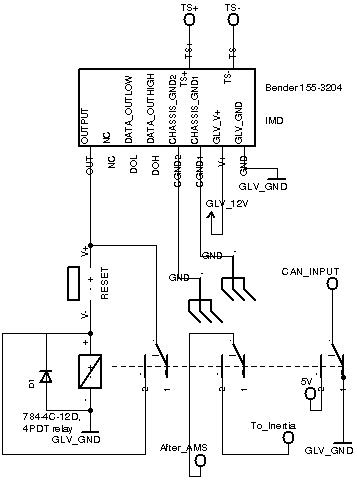
\includegraphics[width = 0.4 \textwidth]{Only_IMD}
                \caption{\hlr{Schematic of the IMD and its connections}}
                \label{IMD}
            \end{figure}

            The IMD output powers a four pole double throw relay. However, for the relay to become powered,\hlr{at the start of each driving/operable session (not when there is a fault in the shutdown system)}, a person must press the IMD reset button, which closes the circuit and allows the coil to power itself through the first pole. \hlr{The other two poles close the shutdown circuit and the input pin to the CAN node. The fourth pole is not connected. The can input will inform the CAN system about the status of the IMD (pull up resistor ensures IMD CAN pole input is not left floating). The ATmega16M1 controls the IMD light in the cockpit through the CAN system. With the coil powered from the IMD's positive output, the shutdown circuit will close. }

            The connectors used for the IMD are the TYCO-MICRO MATE-N-LOK 1 x 2-1445088-8 and its mate.

            %connectors and cables used? Useful data regarding the wiring, including wire gauge/temp.voltage rating and fuses protecting the wiring

        \subsubsection{Position in Car}

            As part of the shutdown circuit, the IMD will be located inside the enclosure shown in Figure \ref{cpanel2}. This is a convenient location for the IMD as high voltage sensing lines must already be present here for the TSMP's.

    \subsection{Inertia Switch}

        \subsubsection{Description (Type, Operation Parameters)}

            The Sensata Resettable crash sensor (6-11g version) will trigger due to an impact that decelerates the vehicle at between 6-11g.

    \begin{table}[H]
    \centering
    \begin{tabular}{|l|l|}
    \hline
    Inertia switch type & Sensata 6-11g crash sensor \\ \hline
    Supply voltage range & \hlr{12} VDC \\ \hline
    Supply voltage & 12VDC \\ \hline
    \begin{tabular}[c]{@{}l@{}}Environmental temperature\\ range\end{tabular} & -10-120 \degree C \\ \hline
    Maximum operational current & \begin{tabular}[c]{@{}l@{}}20A for max. duration 30sec, \\ 10A max. continuous\end{tabular} \\ \hline
    Trigger charactersitics & \begin{tabular}[c]{@{}l@{}}Operate above 11g peak, 60ms duration\\ Not operate below 6g peak, 60ms duration\end{tabular} \\ \hline
    \end{tabular}
    \caption{Parameters of the Inertia Switch}
    \label{InertiaTable}
    \end{table}

        \subsubsection{Wiring/Cables/Connectors}

            \hlr{The Inertia switch will be wired to be normally closed and open the shutdown circuit in the case that there is a crash. The inertia switch is wired in-line with the shutdown circuit to be normally closed. Please see figure} \ref{switchesonly} \hlr{for the position of the IMD in relative to the other shutdown system components. }

                %connectors and cables, useful wiring data?

            % \begin{figure}[H]
            %     \centering
            %     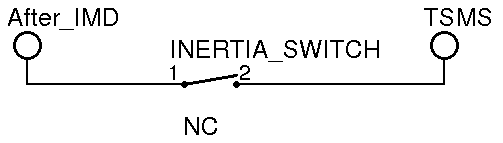
\includegraphics{inertia}
            %     \caption{\hlr{Schematic of the inertia switch and references to where it is in the shutdown circuit}}
            %     \label{inertia}
            % \end{figure}

            % \begin{figure}[H]
            %     \centering
            %     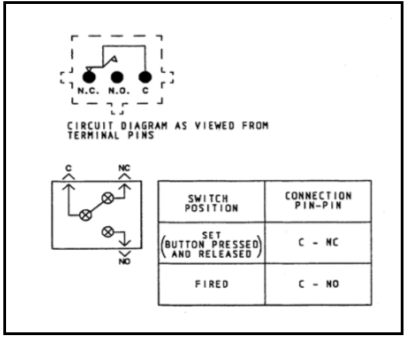
\includegraphics[width = 0.5 \textwidth]{sensatawiring}
            %     \caption{Wiring example for the Inertia switch, see appendix for full datasheet}
            %     \label{wiringinertia}
            % \end{figure}

        \subsubsection{Position in Car}

        The inertia switch will \hlr{be located on the dashboard, in reach of the driver as to fit EV5.7.4.}

    \subsection{Brake Plausibility Device (BSPD)} \label{BSPD}

        \subsubsection{Description/Additional Circuitry}

The BSPD will constantly check if there is a substantial amount of current across the motor controllers and if the brakes are being pressed hard. If both are true, after 0.5 second of continuity, the relay will open the switch in the shutdown circuit. The circuitry consists of an AND gate with two hall effect sensors and the brake sensor as inputs and a 555 timer to check if the states of both the brakes and the motor controllers are continuous. Two hall effect sensors had to be used, as not once outside of the accumulator does the TS wiring all go through one wire.


            \begin{table}[H]
                \centering
                \begin{tabular}{|l|l|}
                \hline
                Brake sensor used: & Pegasus Brake Light switch, part 3601 \\ \hline
                Torque encoder used: &  Active Sensors MHR5621\\ \hline
                Supply voltages: & 5V \\ \hline
                Maximum supply currents: & 15 mA\\ \hline
                Operating temperature: & -55 to 150 \degree C \\ \hline
                Output used to control AIRs: & TE Connectivity Relay, part PB766-ND \\ \hline
                \end{tabular}
                \caption{Torque Encoder Data}
                \label{TorqueEncoder1}
            \end{table}

        \subsubsection{Wiring}

            \begin{figure}[H]
                \centering
                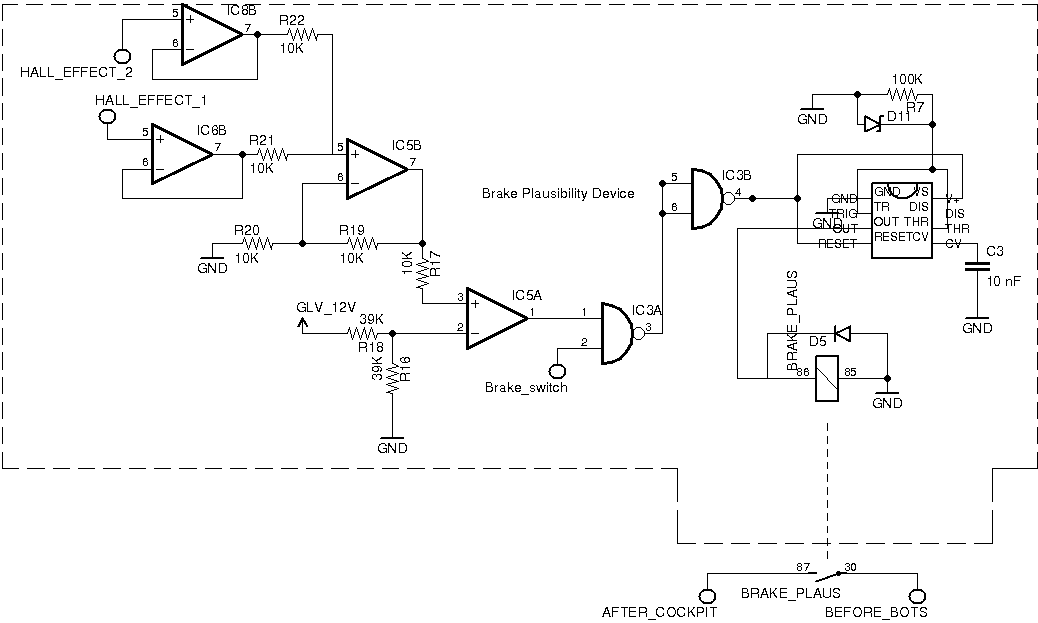
\includegraphics[width = 0.9 \textwidth]{BSPD}
                \caption{Schematic of the BSPD}
                \label{BSPDschem}
            \end{figure}

A Hall effect current sensor, wired before the current splits to the motor controllers, will send a proportional signal to a comparator. If the current is above 50 Amps, the output will be positive, and a positive signal will be sent to the AND gate. If the brakes are actuated, a positive signal will come from the brake pressure switch, causing the AND gate to return positive. These signals will go to two 555 timers, causing a time delay of .5 seconds. If the signal is maintained over this time period, \hlr{the normally open relay will be opened}, shutting down the current to the AIRs.

            %INcluding the circuit board? Show data regarding the cables and connectors used, and how this opens the shutdown circuit

        \subsubsection{Position in Car/Mechanical Fastening/Mechanical Connection}
 The brake sensor is Pegasus Racing P/N 3601 pressure switch that activates between 60 and 120psi. It is attached to the brake line using a -3 AN T-fitting. The brake system is composed of a combination of hard and flexible brake line and will use a combination of SAE flare connections and AN fittings.

            The circuit board controlling the BSPD is located \hlr{near the throttle and brake lines, in the bulkhead of the vehicle}. The board will be positively retained in the enclosure using standard hardware and stand-offs, \hlr{all external connections will be made using Ampseal connectors} and all internal enclosure connections will be made using Molex PCB connectors. \hlr{Figures} \ref{BSPDmech1} \hlr{and} \ref{BSPDmech2} \hlr{show how the brake sensor will be mounted and where it will be located. }

            \begin{figure}[H]
                \centering
                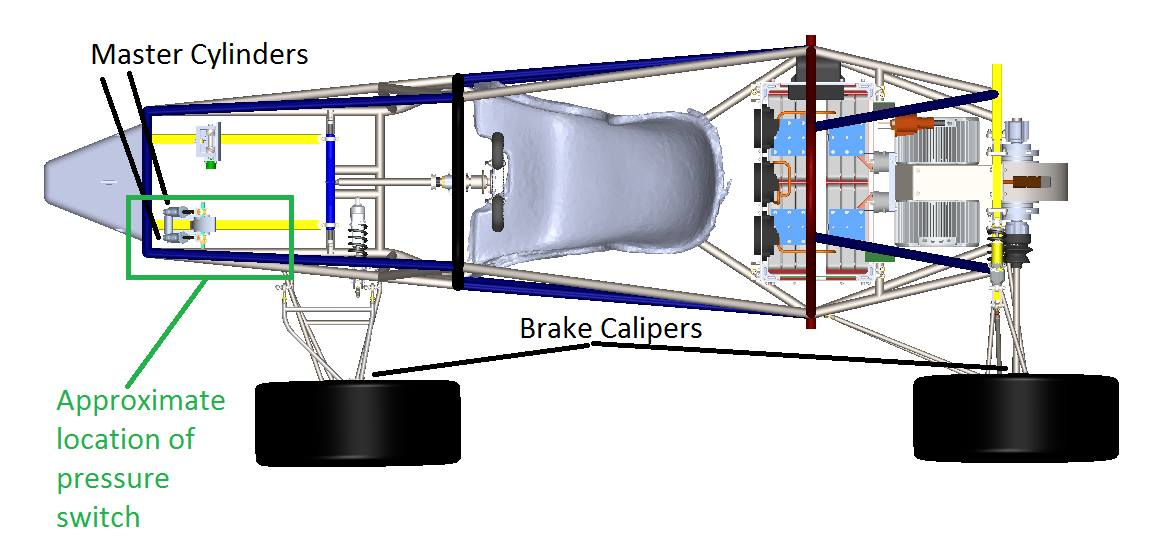
\includegraphics[width = 0.9 \textwidth]{brakeincar}
                \caption{View of BSPD Pressure Switch and T-Fitting}
                \label{BSPDmech1}
            \end{figure}

            \begin{figure}[H]
                \centering
                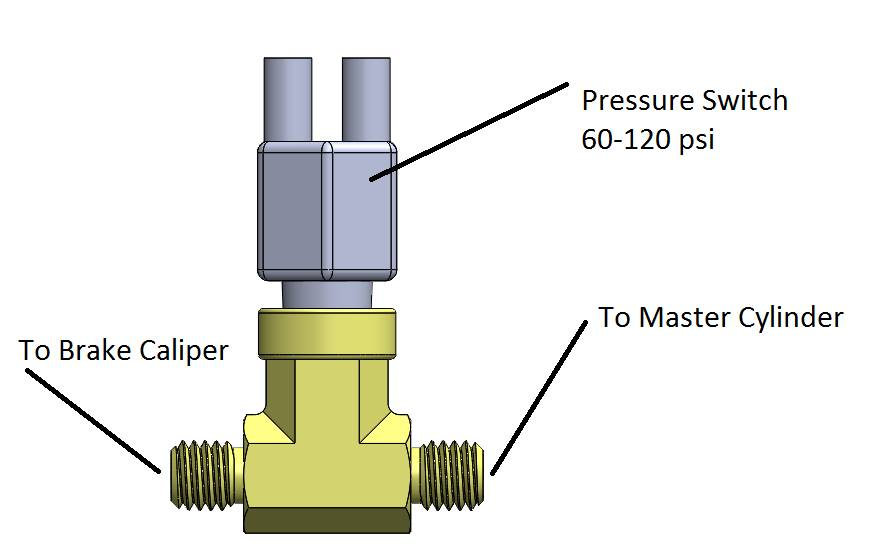
\includegraphics[width = 0.9 \textwidth]{brakesensor}
                \caption{Approximate Location of BSPD Pressure Switch in Vehicle}
                \label{BSPDmech2}
            \end{figure}

    \subsection{Reset/Latching for IMD and BMS}

        \subsubsection{Description/Circuitry}

            %Describe the concept and circuitry of the latching/reset system for a tripped IMD or BMS.  Describe the method for resetting the IMD and BMS.

            If the AMS detects a fault. It opens the shutdown circuit, and latches into that state. When the AMS reset \hlr{button} is pressed, the nearby CAN node passes a "Reset" CAN message to the AMS boards. If the accumulator is within safe electrical and temperature operating limits the AMS closes the shutdown circuit.\\

           To reset the IMD an operator other than the driver must push the IMD reset button located on the outside of the car on a panel next to the TSMPs, master switches and E-stops. If the output of the IMD is high because there is no ground fault, the reset button will activate the coil and close the shutdown circuit.

        \subsubsection{Wiring/Cables/Connectors}

            %Calcs for connectors and cables used and how they open the shutdown circuit
            The IMD's output, as seen in figure \ref{IMD}, continuously closes the shutdown circuit as long as its output is high. The reset button closes the circuit to the coil to then allow the coil to power itself for as long as the output is high. Once low, the coil will open its four poles, thereby \hlr{not allowing power to the CAN node input, thereby activating the IMD light} or the switch in the shutdown circuit. The 4PDT relay is specified for 15A, while the GLV system it controls is fused for 4A. The wire gauge to the IMD relay is 22AWG.\\

            % BMS reset wiring
            The BMS reset button is a button that connects 5V to a CAN input pin on the \hlr{side panel} node later mentioned in section \ref{imdnode}. When the CAN node receives a high signal it sends a message to the rest of the system, including the AMS nodes, and if the AMS detects the accumulator is safe, the AMS relay will close the shutdown circuit and allow normal operation. All wire gauges will be 22 AWG except for PCB traces. Because CAN communication requires very little current, the lines will not be fused.\\

            The connectors used \hlr{for the IMD} will be Molex, LLC 0022013037 and its pair, Molex, LLC 0022232031, or other Molex products of the same series but with a different number of headers on each side of the connector.

        \subsubsection{Position in Car}

            The IMD and BMS reset buttons will be panel mounted to the enclosure shown in Figure \ref{cpanel2}. The AMS will be within the accumulator container.

    \subsection{Shutdown System Interlocks} \label{interlocks}

        \subsubsection{Description/Circuitry}

            %Concept and circuitry
            %Note: Interlocks are circuits used to open the shutdown circuit if a connector is disconnected or enclosure is opened.  This is not the entire shutdown circuit.
            Interlocks are low voltage mechanically activated switches that close when a high voltage connection is made or a system is closed.  In the shutdown circuit, \hlr{the main accumulator connectors, and the HVD} have interlocks. The shutdown circuit will be open when any of these TS connections are opened. \hlr{There is also an interlock on the charger connector that bypasses the main battery connector interlocks.}

        \subsubsection{Wiring/Cables/Connectors}

            Interlock wires are mechanically integrated with HV connectors such that they are simultaneously disconnected with the removal of a connector. The removal of a connector therefore breaks shutdown circuit continuity. \hlr{The interlock wires will be 22 AWG and be fused from the shutdown GLV fuse (2A).}

            \begin{figure}[H]
                \centering
                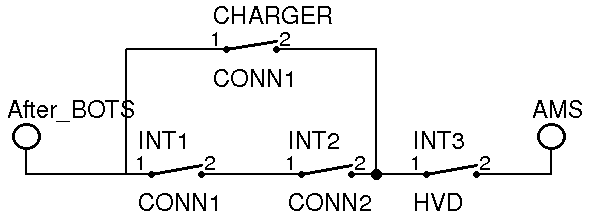
\includegraphics{interlocks}
                \caption{\hlr{Interlocks contained in the shutdown circuit}}
                \label{interlockschem}
            \end{figure}

        %    \begin{figure}[H]
        %        \centering
        %        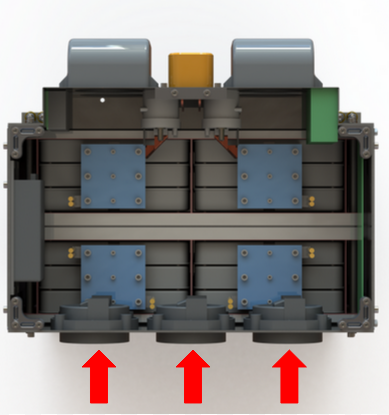
\includegraphics[width = 0.3 \textwidth]{MSD}
        %        \caption{MSDs in the accumulator, indicated by the red arros}
        %        \label{MSDs}
        %    \end{figure}

        \subsubsection{Position in Car}

            Interlocks are contained within the main accumulator two-pole HV connector (labeled CONN) and the HVD. Both connections are out of the accumulator, and located in the back of the car. Please see section \ref{hvdsection} for details.

            There is a charger interlock that overrides (in parallel with) the main connection interlocks. This interlock is only used during charging.

    \subsection{Tractive system Active Light}

        \subsubsection{Description/Circuitry}

            \begin{figure}[H]
                \centering
                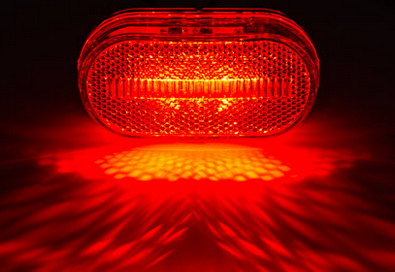
\includegraphics[width = 0.5 \textwidth]{TSALshining}
                \caption{Product picture of the TSAL, from Super Bright LEDs part no. M9-R4}
                \label{tsalsuperbright}
            \end{figure}

            The TSAL illuminates when the tractive system is active, which is defined as the tractive system voltage being over 60V or the AIRs being closed.

            \begin{table}[H]
                \centering
                \begin{tabular}{|l|l|}
                \hline
                Supply voltage: & 12V \\ \hline
                Max. operational current: &  0.04A\\ \hline
                Lamp type & LEDs \\ \hline
                Power consumption: & 0.48 W\\ \hline
                Brightness & Unknown \\ \hline
                Frequency: & Manual with 555 timer, 2.4 Hz \\ \hline
                Size (length x height x width): & 103x27x51 mm \\ \hline
                \end{tabular}
                \caption{Parameters of the TSAL}
                \label{TSALparameters}
            \end{table}

        \subsubsection{Wiring/Cables/Connectors}

            %Describe wiring, show schematics, describe connectors and cables used and show useful data regarding the wiring.  Include gauge, voltage and temperature rating of wiring used and any fuses or other overcurrent protection used.

            There is a DC-DC (isolated) converter that converts TS 100V to 12V for the light. \hlr{The DC-DC converter accepts 16-166VDC as input voltage.} This will power a 555 timer astable circuit. When the TS is over 60V, zener diodes with a breakdown voltage of 56V and 3.6V respectably power one side of an optocoupler when the TS voltage is over 60V. The optocoupler closes the circuit on the other side for the timer's output to go to the light through an OR gate. The OR gate also accepts the GLV 12V as an input, which is only live when both AIRs are closed. In this way, the light will be powered when the tractive system is over 60V or the AIRs are closed. The light will blink at 2.4 Hz.
            %Should we have a fuse before the OR gate?

            \begin{figure}[H]
            \centering
            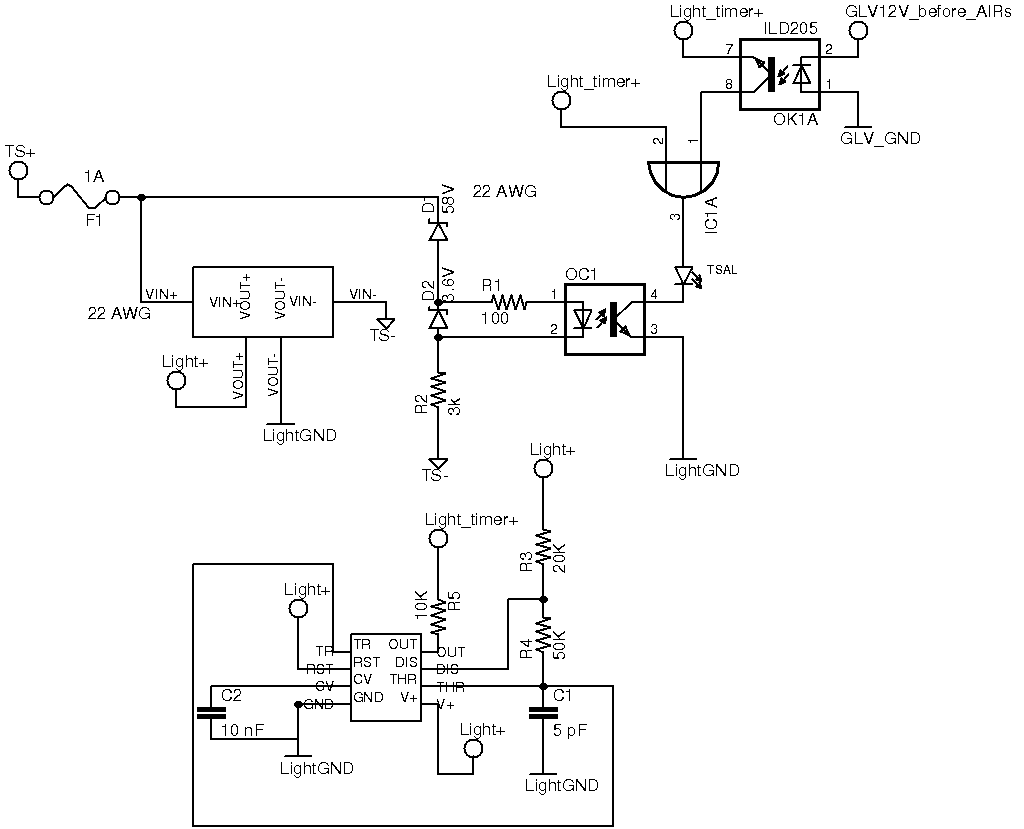
\includegraphics[width = 0.7 \textwidth]{TSAL_FSAE}
            \caption{\hlr{Schematic for the TSAL}}
            \label{TSALschem}
            \end{figure}

            As shown in Figure \ref{TSALschem}, there is a 1A fuse protecting both the DC-DC converter and the light's optocoupler. There is a fuse not shown that is in the GLV system, which protects the GLV 12V shown before the AND gate. All connections made by wires will be 22 AWG rated for 600V, 125 \degree C and 7A, while all PCB traces will be a minimum of 10 mil, but nominally 20 mil in width.

            %highlight the caption of the replacement picture.
            % \begin{figure}[H]
            %     \centering
            %     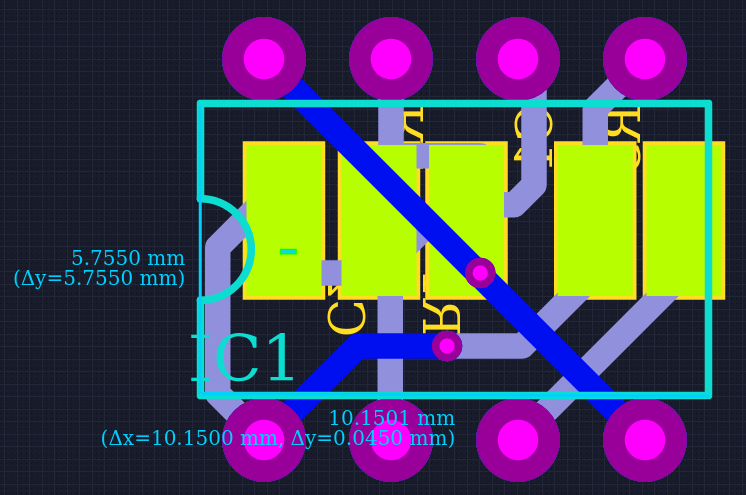
\includegraphics[width = 0.7 \textwidth]{OscillatorPCB}
            %     \caption{PCB for the oscillation circuitry}
            %     \label{oscillationpcb}
            % \end{figure}

        \subsubsection{Position in Car}

            The TSAL will be mounted to the underside of the highest point of the main roll hoop, per EV 4.12.4 using a robust 3D printed bracket integrating the light and necessary wiring. This enclosure has not been designed yet.

            The PCB will be located in the side panel enclosure, also known as the TSMP housing.

    \subsection{Measurement Points}

        \subsubsection{Description}

            %Describe the housing used and how it can be accessed, etc.  Describe how the measurement points protected/covered when not in use and how the electrical connections on the back of the measurement points are protected when the measurement points are being used.

            The TSMPs and GLVS ground measuring points are housed in a non-conductive, well-marked housing that can be opened without tools. It will be protected from people touching it by shrouded banana jack connectors. The measuring points allow for safe measurement of the tractive system voltage and for manual detection of ground faults.The TSMPs will be in the same housing as the side panel CAN node and PCB.

        \subsubsection{Wiring, Connectors, Cables}

            \begin{figure}[H]
                \centering
                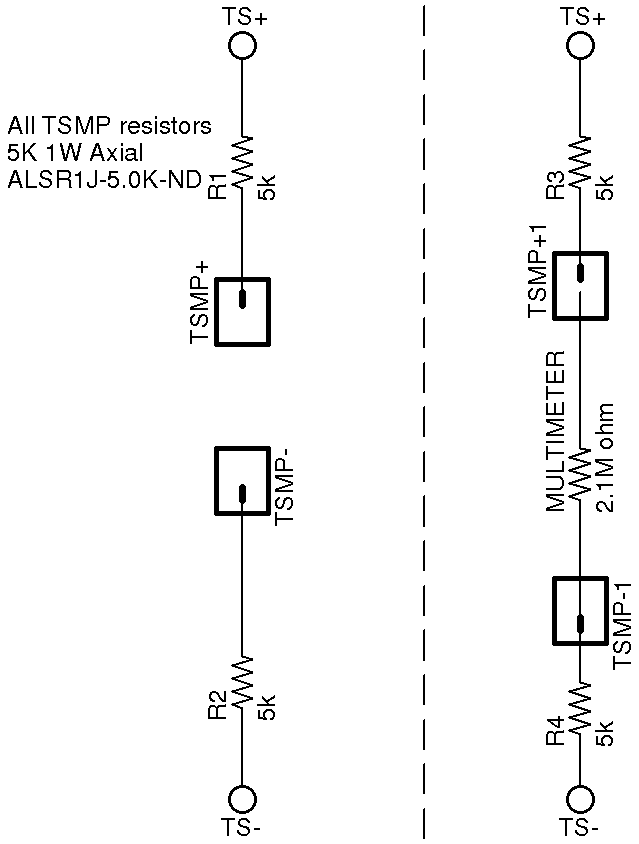
\includegraphics{TSMP}
                \caption{Tractive System Measuring Points}
                \label{fig:TSMPschematic}
            \end{figure}

            Figure \ref{fig:TSMPschematic} shows the TSMP schematic. Left shows the schematic including the banana jacks. Right shows the multimeter measuring the tractive system, with the multimeter's expected resistance and the same resistors as before the TSMP's on the left side.\\

            There will be four measuring points: TS+, TS-, GLV+, and GLV-. The TSMP connections will be secured with 5 k\ohm current limiting resistors. There will not be a fuse. The worst case scenario for the TSMPs occurs when there is a short between the TS+ and TS- banana jacks. This could occur as a result of operator error when measuring the TS  voltage and create a voltage over a human operator's hands. The current limiting resistors ensure that the current draw in this scenario will not harm a human.

            \begin{align}
                V = I * R \\
                100 V = I * 10,000 \ohm \\
                I = 0.01A
            \end{align}

            \begin{align}
                P = I * V \\
                P = 0.01 I * 100V V \\
                P = 1 W
            \end{align}

            Therefore, a 1W, 5k\ohm resistor will be placed before each TSMP banana jack. The resistor will be on \hlr{the side panel PCB, which contains all of the low current TS circuitry and certain shutdown components. The TS line going to the side panel is fused, with a rating of 1A, within the accumulator, and then the 22 AWG shielded wire is connected to the side panel PCB for the TSMP resistors.} This PCB does not have a finished design yet, but will be housed such that it is insulated from all adjacent conductive materials.\\

            Another worst case scenario that could occur at the measuring points is a short between the TS and GLV systems over the banana jacks, again by operator error. In this scenario, the IMD will open the shutdown circuit.

            \hlr{The TSMP banana jacks are 72930-2 and 72930-0 Pomona Electronics 4 mm banana jacks (red and black, respectively). The TSMP resistors are Vishay Dale, ALSR035K000FE12 (manufacturer's part number), rated for V and part of the ALSR/ALVR series. The datasheets for both the banana jacks and the resistors can be found in section} \ref{tsmpappendix}.

            %Describe wiring, show schematics, and describe connectors and cables used and show useful data regarding the wiring.  Include details on the protection resistor including resistance, voltage and power rating.

        \subsubsection{Position in Car}

            The TSMP's will be located in the enclosure shown in Figure \ref{cpanel2} \hlr{along with the side panel circuitry}. Body panel removal will not be required for access, and any protective covers for the TSMP's will be removable without the use of tools. \hlr{The enclosure itself is bolted together using 1/4" hardware.} %, but we intend to provide additional banana jack measuring points to measure the TSMP resistors without removal of any vehicle components.
            %I wish we'd have that.

    \subsection{Pre-Charge Circuitry}

        \subsubsection{Description}

            In order to prevent damage to the motor controllers, AIRs, and ultimately the driver, it is important to ramp the tractive system up to full operating voltage rather than instantaneously jump from 0V to 100V. One consequence of an immediate transition to high voltage can be arcing across the AIRs. This can cause pitting in the relay contacts over time and ultimately cause the system to fail. Pre-charging reduces the difference in potential on each side of the relay to prevent arcing and ensure the integrity of the electrical system over many uses.

        \subsubsection{Wiring, Cables, Current Calculations, Connectors}
.
            Once the shutdown circuit is closed, it will immediately power the coils of the normally closed discharge relay, the normally open precharge relay, and the normally open TS- AIR. This opens the discharge relay, and closes the precharge relay and TS- AIR. Instead of connecting Batt+ to TS+ through a current limiting resistor, the precharge relay connects B+ to the key switch terminal on each of the Sevcon motor controllers. When powered by their key switch terminals, the motor controllers charge their internal capacitors up to around 50V for 0.5 seconds, then up to 90V (or another specified voltage) for 0.1 seconds before signaling though the CAN system that the precharge is complete. This CAN message causes a node in the battery to allow the shutdown circuit to close the TS+ AIR.


        Please note the schematic in figure \ref{prechargeschem}.

        \begin{sidewaysfigure}[p]
            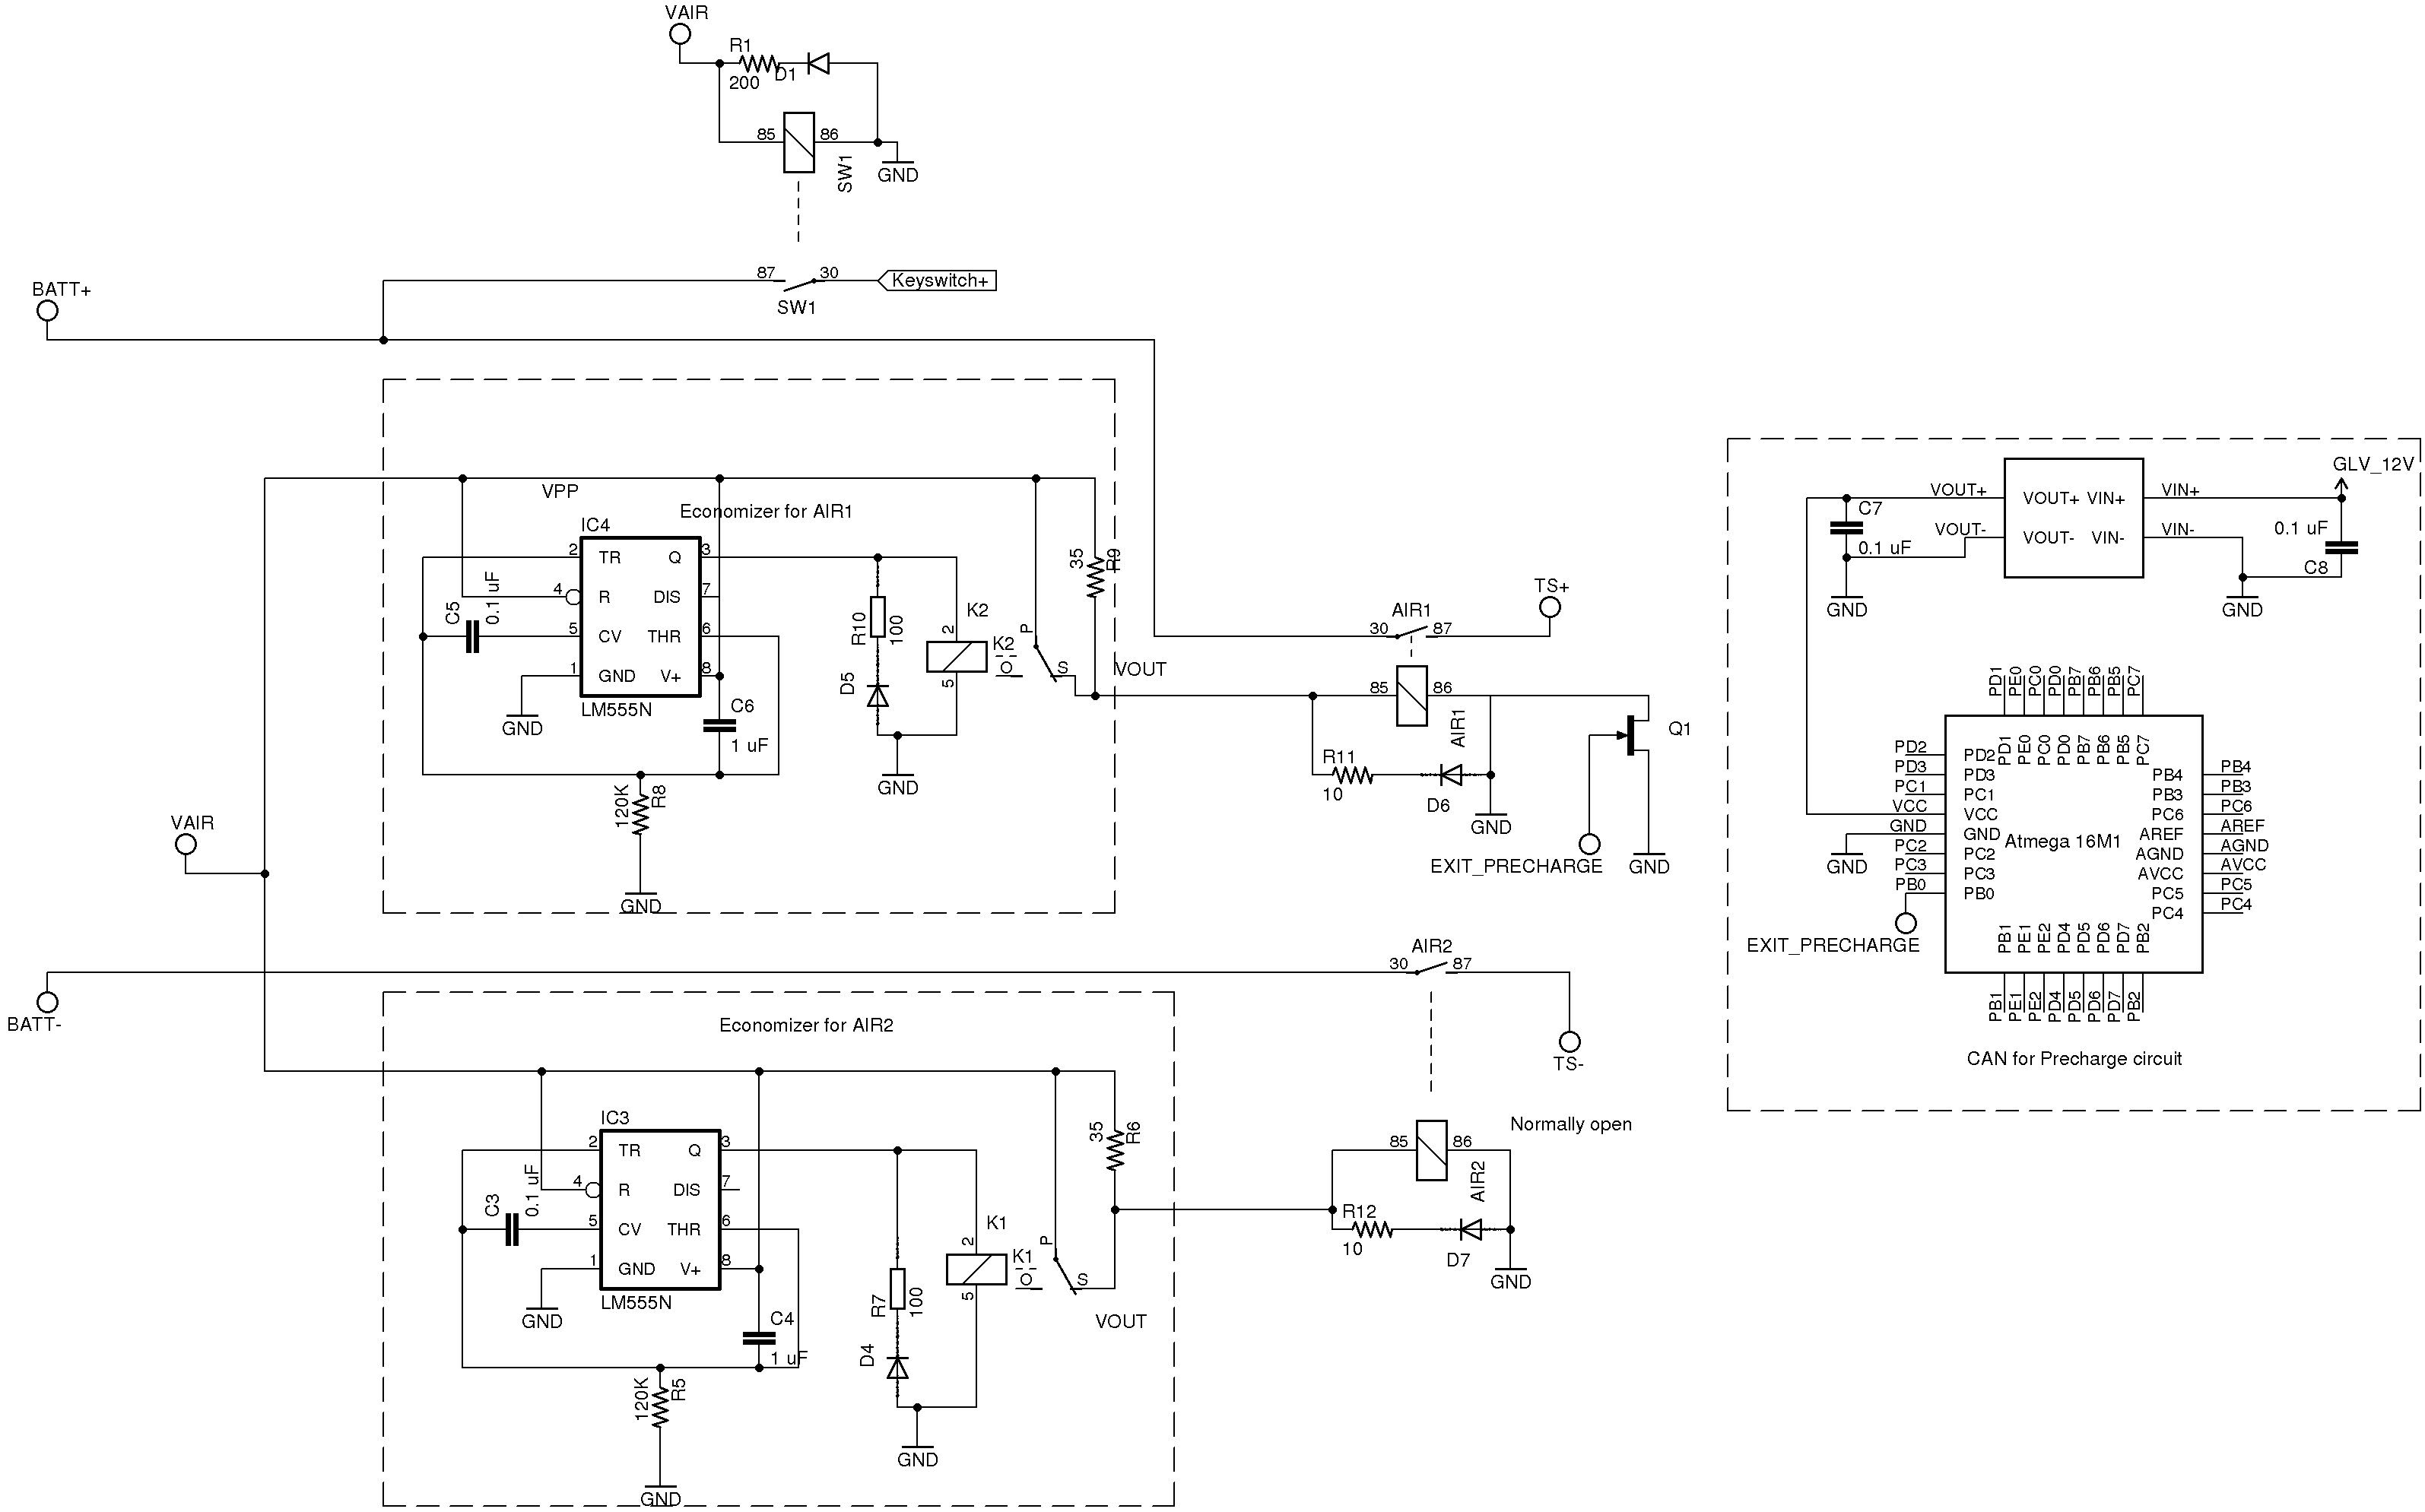
\includegraphics[width=\textheight]{precharge}
            \caption{\hlr{Precharge system schematic, including the AIR economizers}}
            \label{prechargeschem}
        \end{sidewaysfigure}

            \begin{figure}[H]
                \centering
                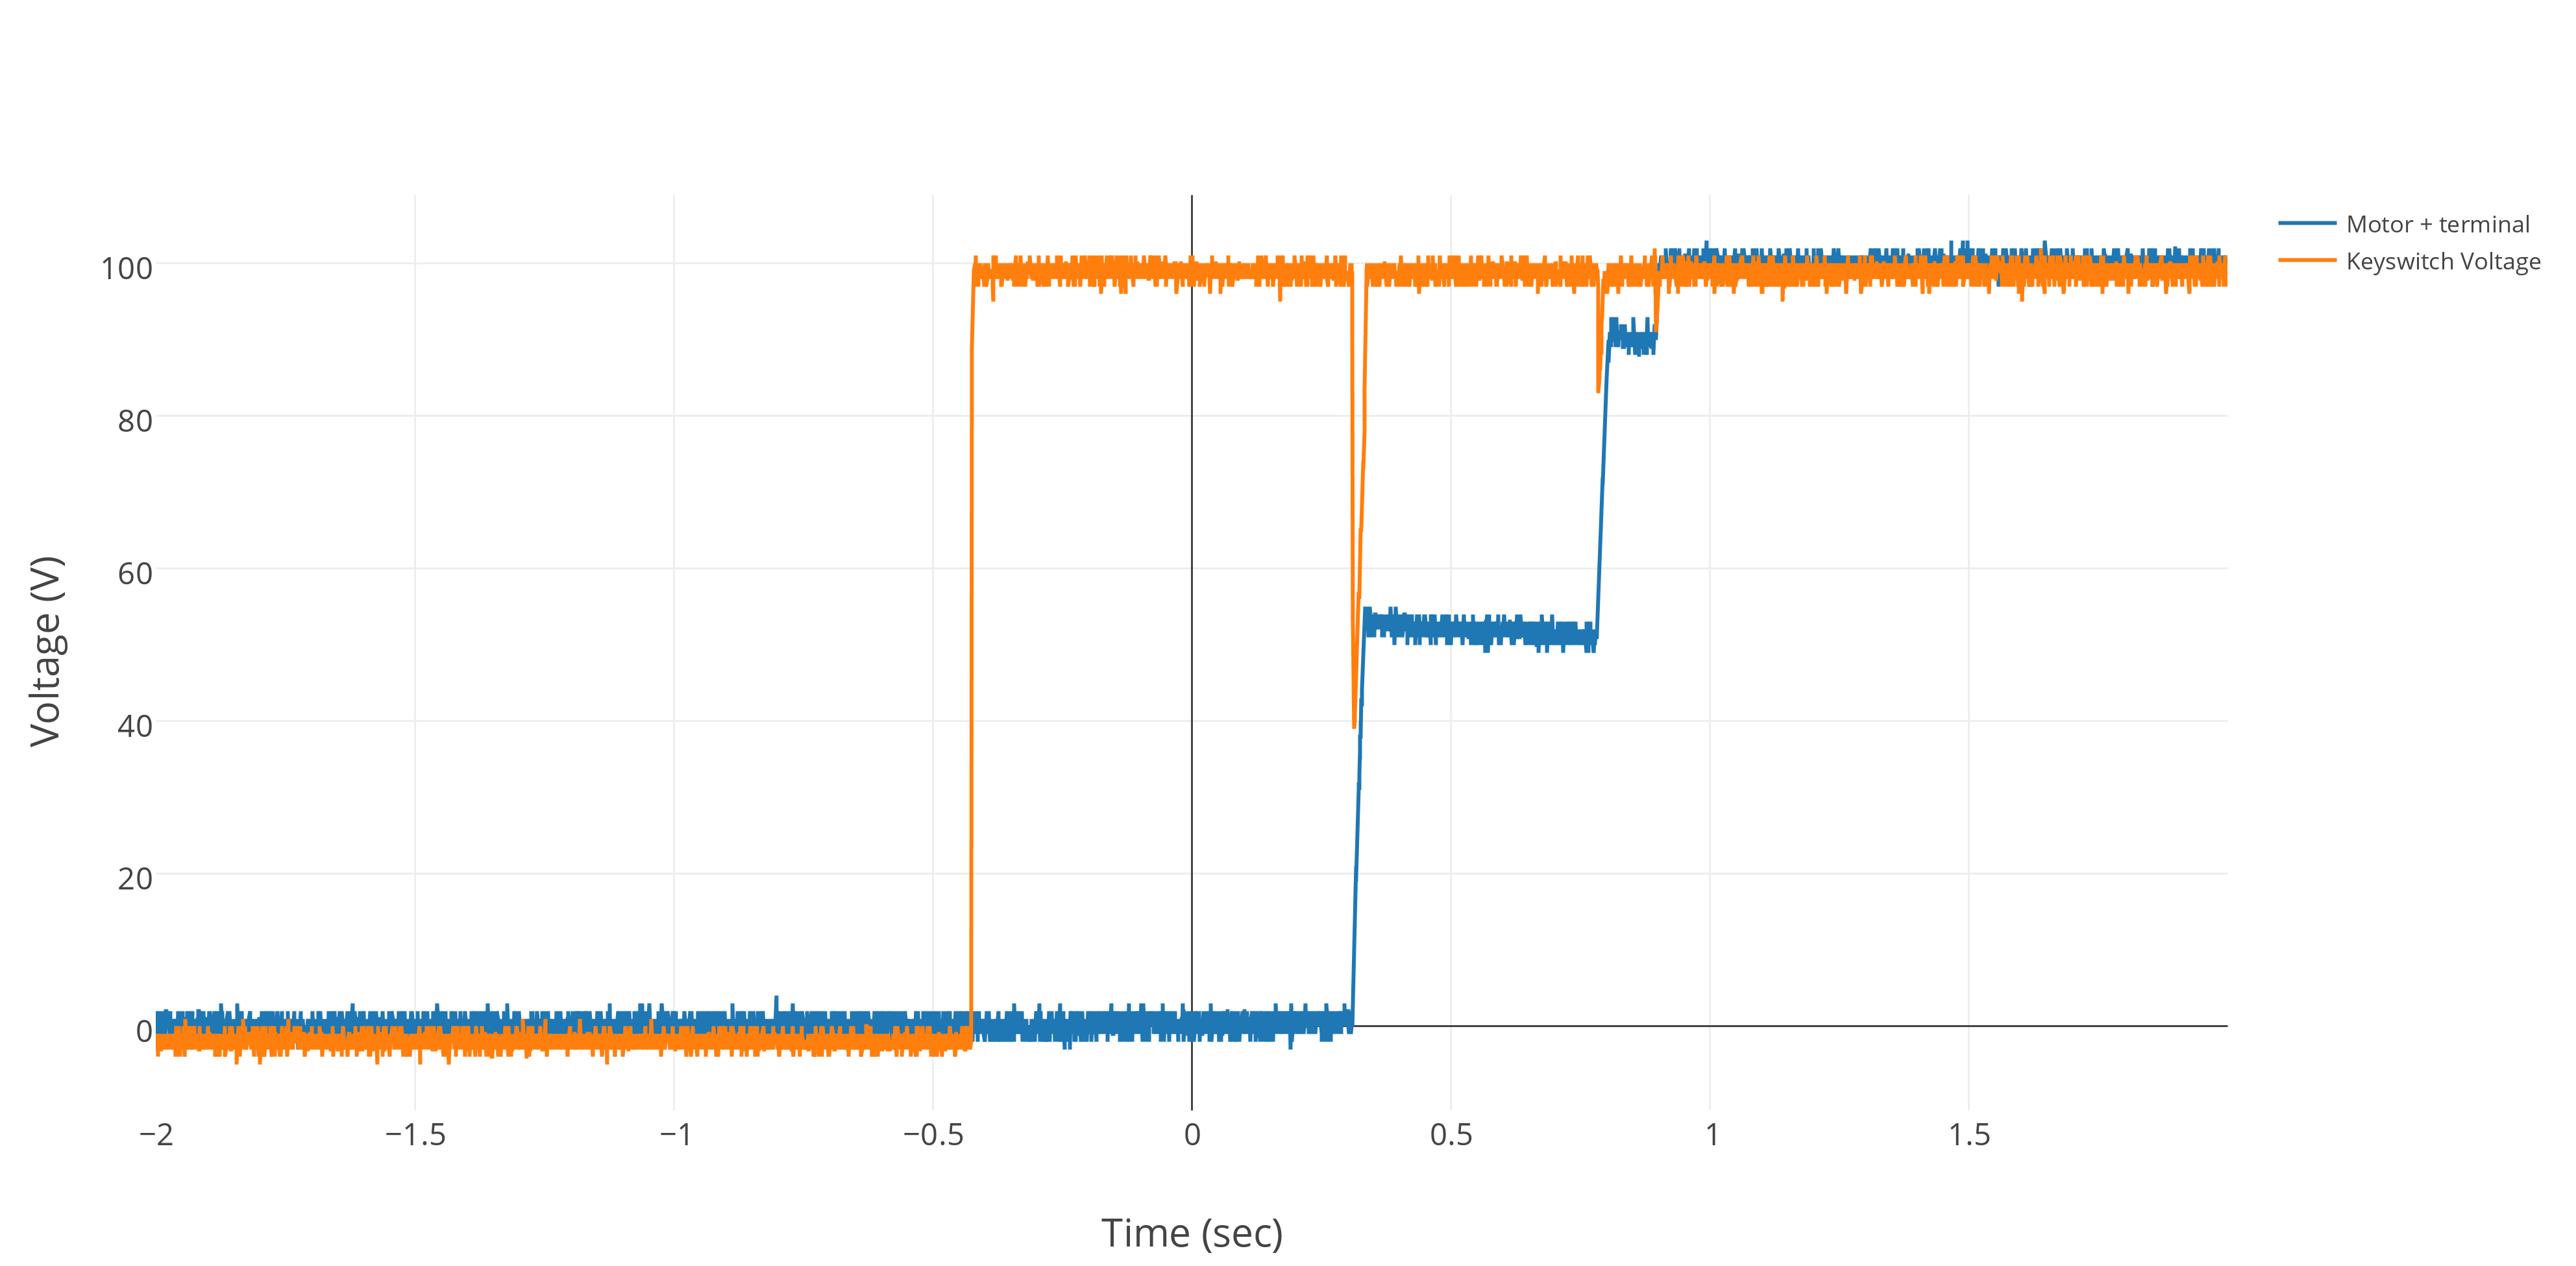
\includegraphics[width = 0.8 \textwidth]{PrechargeVoltage}
                \caption{Voltage vs time, measured in a test setup. }
                \label{PCvoltage}
            \end{figure}

            In figure \ref{PCvoltage}, the voltage of a test setup of the pre-charge system internal to the motor controller was measured. Because there is no resistor other than the motor controller, the current could not be calculated and/or graphed. This was discussed in rules clarification ticket 4487. As discussed above, the function describing the pre-charge is stepwise.

            \begin{table}[H]
                \centering
                \begin{tabular}{|l|l|}
                \hline
                Resistor type & N/A \\ \hline
                Resistance & N/A \\ \hline
                Continous power rating & \hlr{N/A} \\ \hline
                Overload power rating & \hlr{N/A} \\ \hline
                Voltage rating & 150 VDC \\ \hline
                Cross-sectional area of wire used & 0.001275 in\textasciicircum 2 (18 AWG) \\ \hline
                \end{tabular}
                \caption{General data of pre-charge resistor }
                \label{prechargeresistor}
            \end{table}

            %table here of precharge relay

            \begin{table}[H]
                \centering
                \begin{tabular}{|l|l|}
                \hline
                Relay type & \hlr{Omron Electronics, G5CA series, G5LE-14-DC12 part no.} \\ \hline
                Contact arrangement & SPDT \\ \hline
                Continous DC current & 10A \\ \hline
                Voltage rating & \hlr{125VDC} \\ \hline
                Cross-sectional area of wire used & 0.001275 in$^{2}$ (18 AWG) \\ \hline
                \end{tabular}
                \caption{General data of the pre-charge relay}
                \label{PCrelay}
            \end{table}

        \subsubsection{Position in Car}

            The pre-charge circuit is located internal to the Sevcon motor controllers. The position of the controllers in the vehicle is discussed at length in section 5.1.3 and first shown in figure \ref{mcsideview}.

    \subsection{Discharge Circuitry}
    \label{dischargesection}

        \subsubsection{Description}

            %concept
            When the car shuts down, there are still reserves of energy in the tractive system that can be harmful to the driver or team members conducting maintenance. The discharge circuit dissipates the capacitance found in the vehicle after TS shutdown. When the shutdown circuit is opened, the normally \hlr{closed} discharge relay will close a switch and discharge the tractive system with a 220\ohm  power resistor.

        \subsubsection{Wiring, Cables, Current Calculations, Connectors}

            %plot of discharge current vs time
            %formula describing the plot

            \begin{figure}[H]
                \centering
                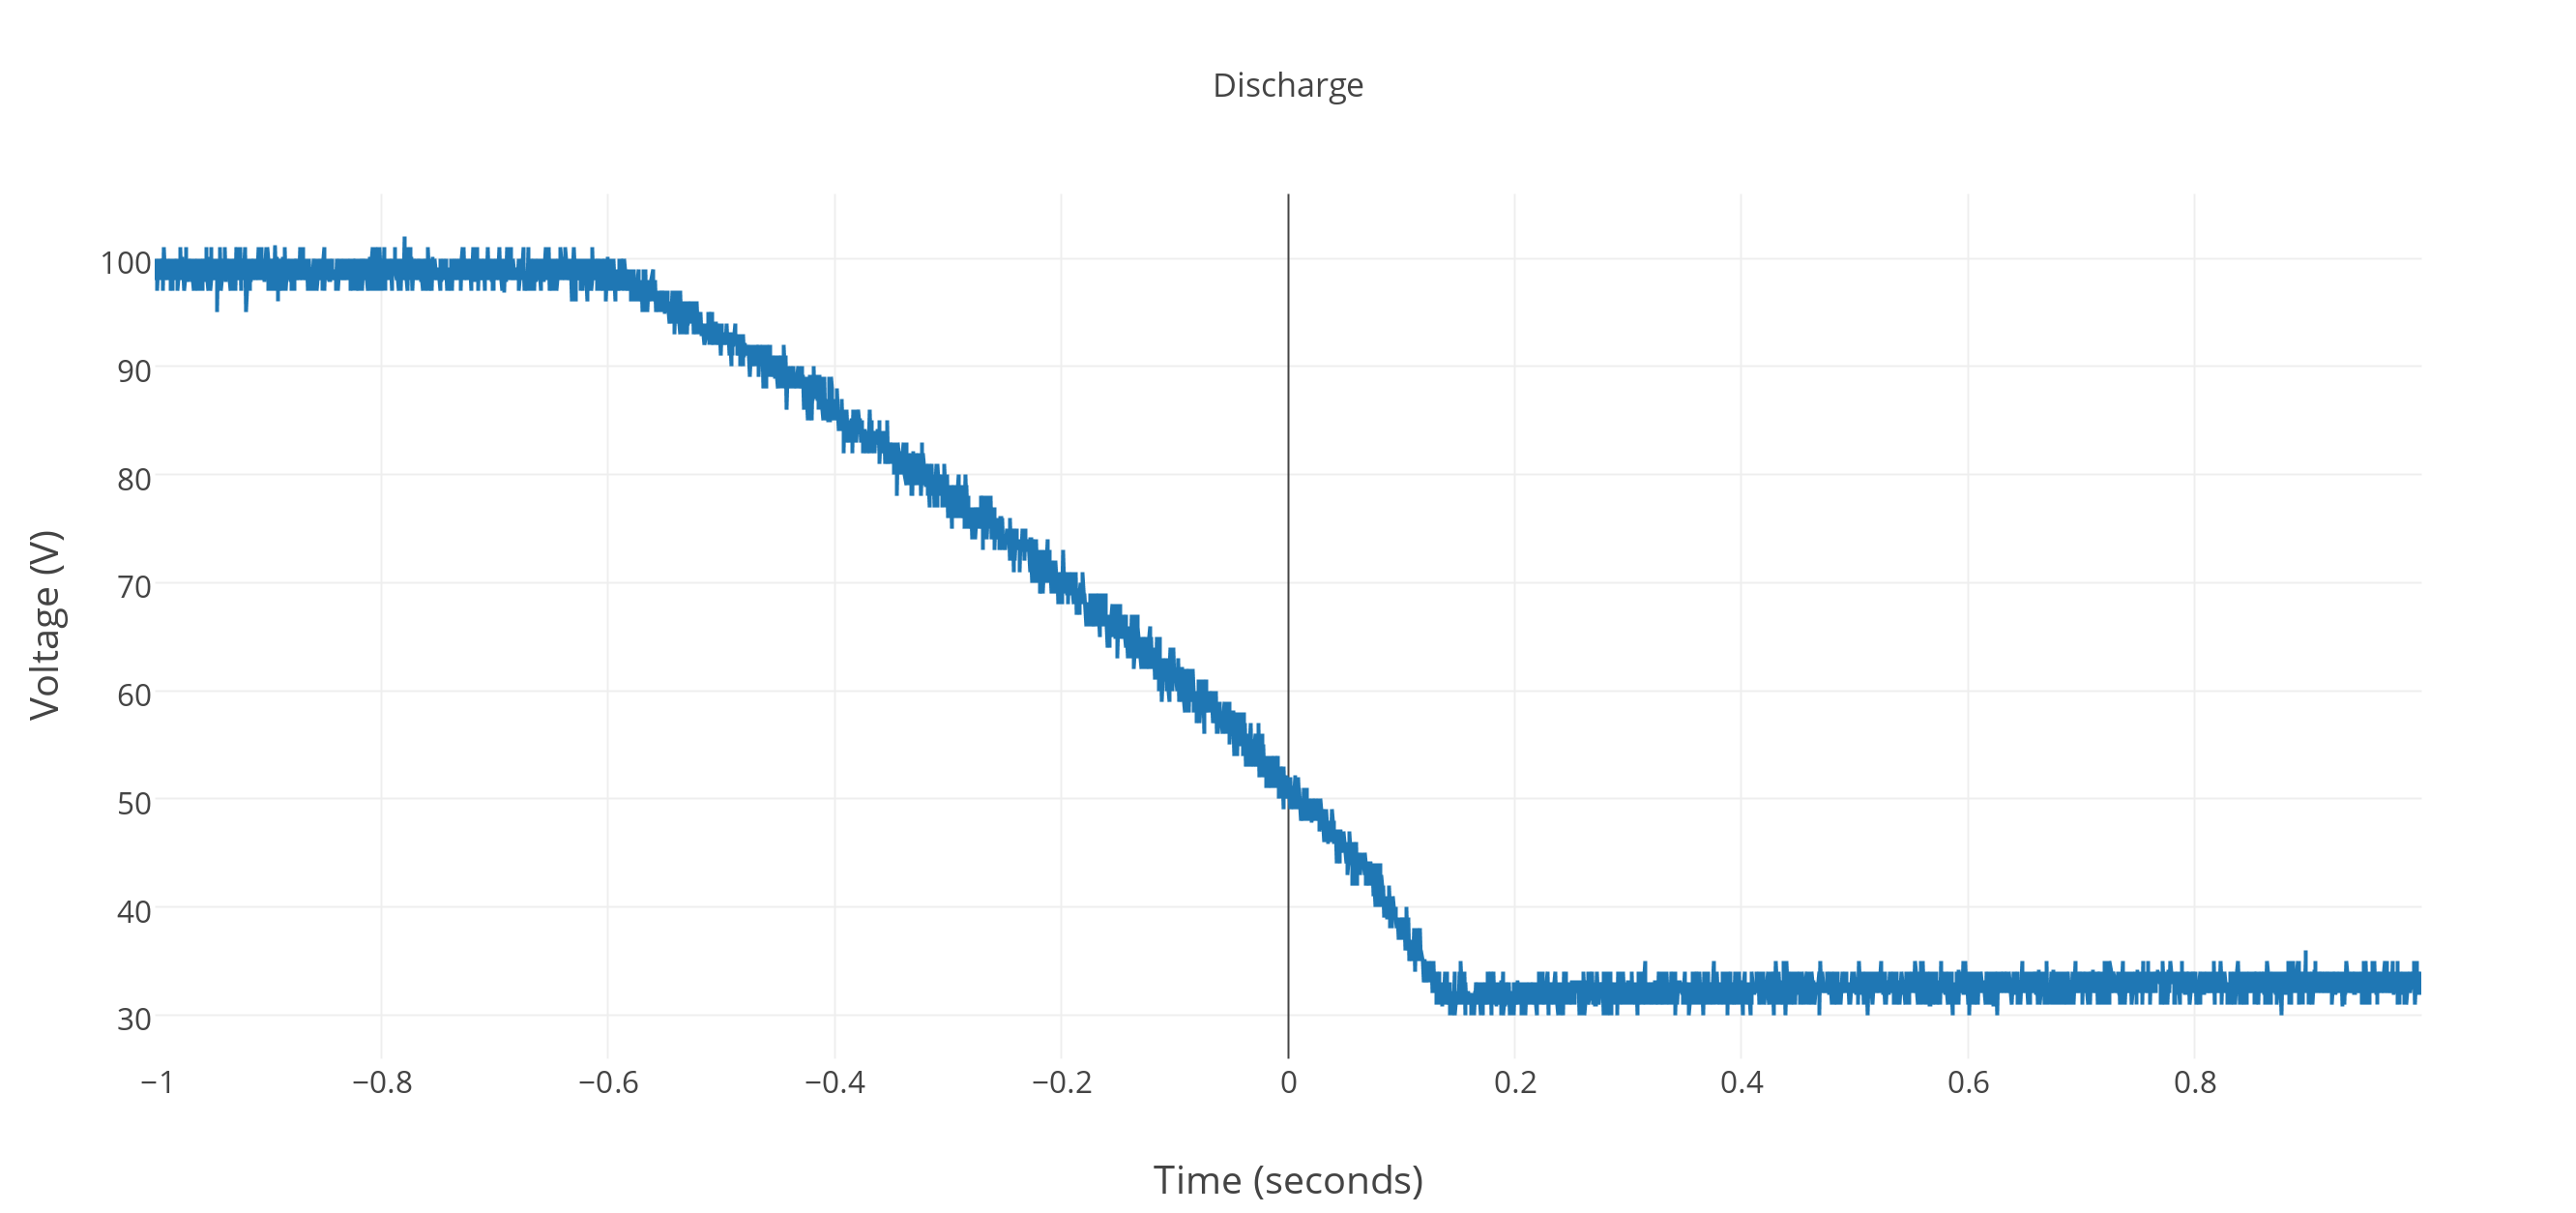
\includegraphics{Discharge}
                \caption{Schematic of the discharge system}
                \label{dischargeschem}
            \end{figure}

            Since the \hlr{internal} capacitance of our motor controllers was unknown, it was determined by the team experimentally.

            \begin{figure}[H]
                \centering
                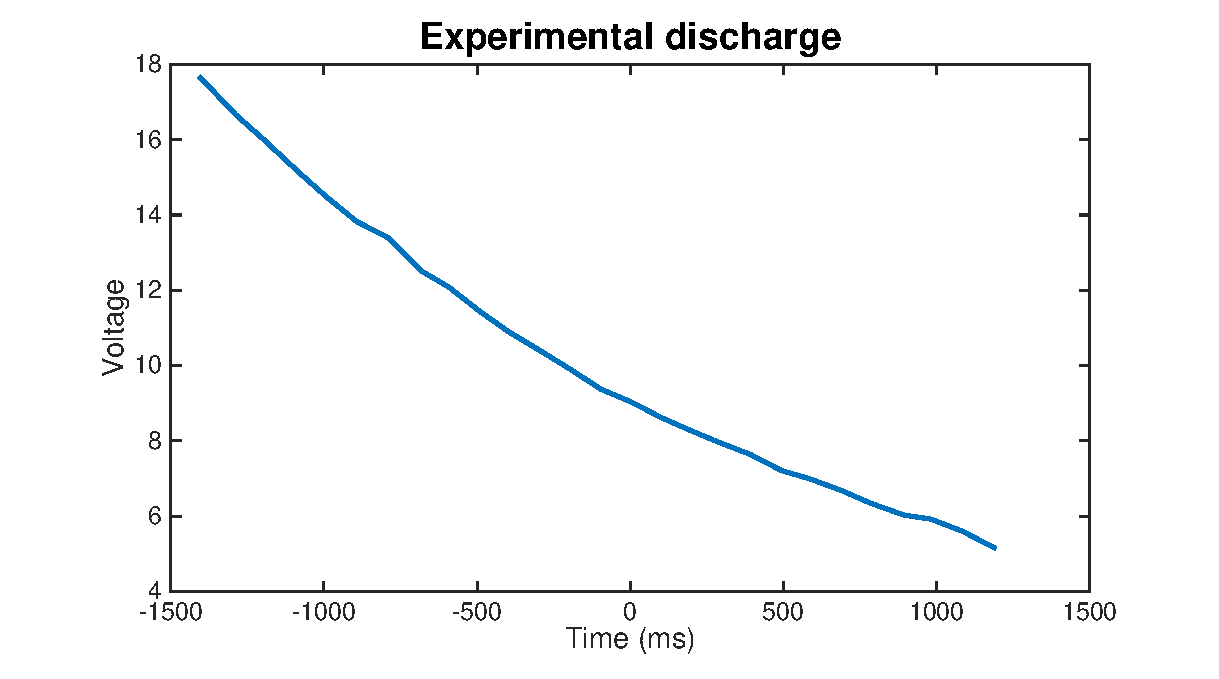
\includegraphics[width = 0.8  \textwidth]{experimental_discharge.eps}
                \caption{A single motor controller being discharged across a known resistor.}
                \label{discharge}
            \end{figure}

            That experimental discharge in figure \ref{discharge} starts at 17.65 volts at a time of -1403 milliseconds. Given that this is an RC parallel circuit, we expect to loose 63\% of the charge in the first RC time constant. The graph hits $17.56 V * 0.37 = 6.53 V$ at 773.5 milliseconds, or in 2.1765 seconds. Given that we know we were discharging with an $846 \Omega$ resistor, we can calculate the internal capacitance of the motor controller.

            \begin{align}
                RC &= 2.1765 s\\
                C &= \frac{2.1765 s}{846 \Omega}\\
                C &= 2.57 mF
            \end{align}

            With that calculation, we can estimate that our two motor controllers will have a combined capacitance of $5.14 mF$ that the discharge circuit needs to handle.

            With a $220 \Omega$ discharge resistor, we can calculate how the discharge will progress over time using the natural response of an RC circuit,

            \begin{align}
                V(t) = V_{0} * e^{-t/RC}
            \end{align}

            \begin{figure}[H]
                \centering
                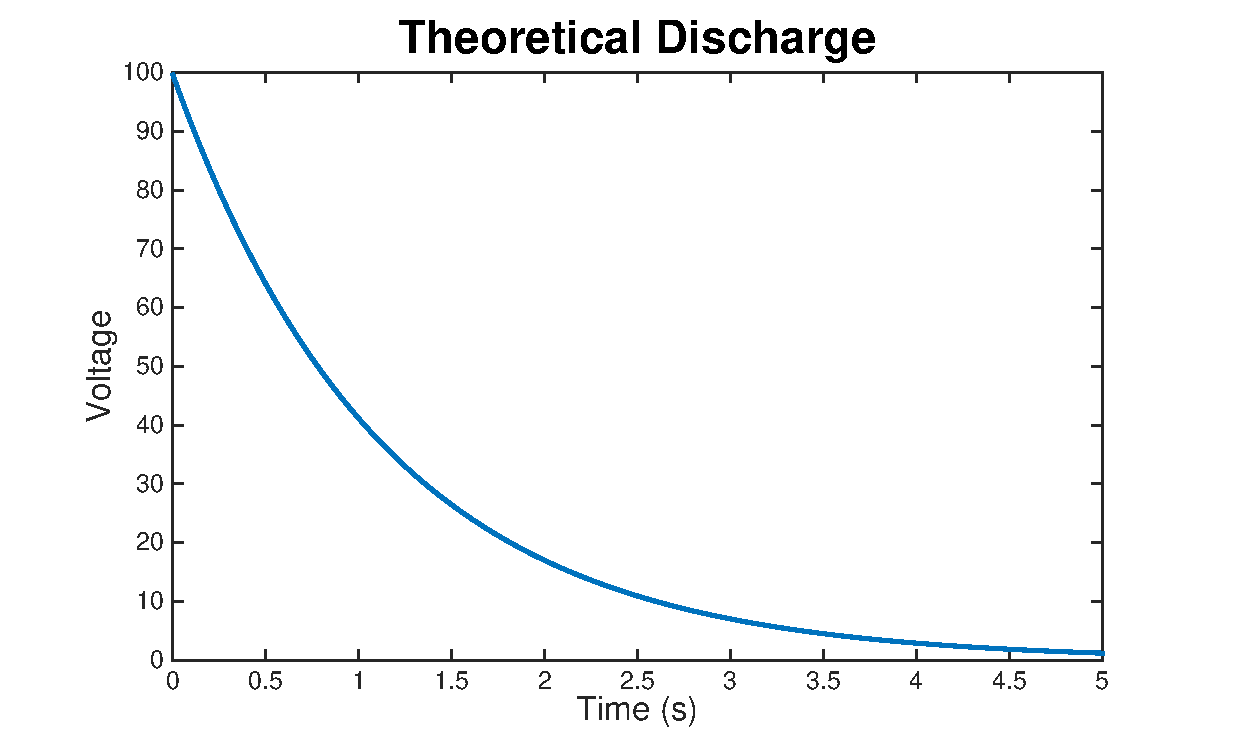
\includegraphics[width = 0.8  \textwidth]{voltage.eps}
                \caption{The theoretical discharge of both motor controllers across the resistor specified in table \ref{dctable}. This calculation shows that we should able to discharge to well under 60V DC in 5 seconds.  }
                \label{discharge_volts}
            \end{figure}

            \begin{figure}[H]
                \centering
                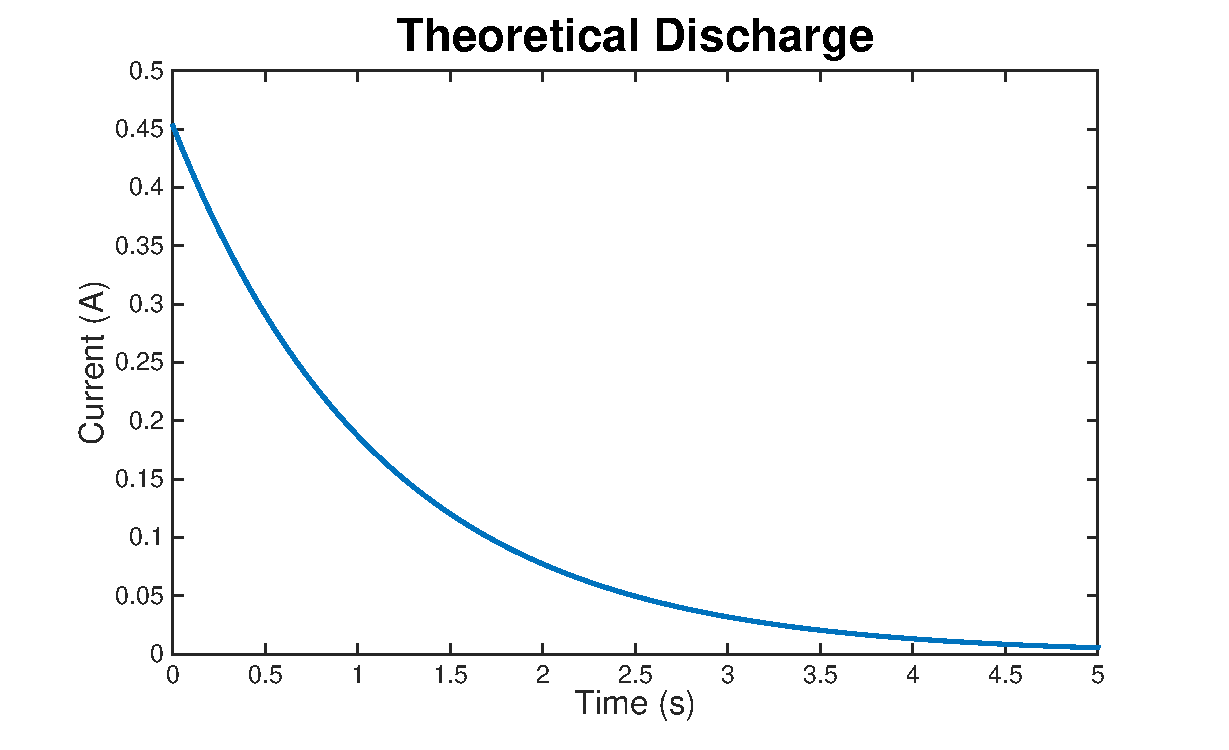
\includegraphics[width = 0.8  \textwidth]{current.eps}
                \caption{The current of the theoretical discharge.}
                \label{discharge_amps}
            \end{figure}

            %table of discharge circuit

            \begin{table}[H]
            \centering
            \begin{tabular}{|l|l|}
            \hline
            Resistor type & \hlr{WH Series, part no. WH50-220RJI} \\ \hline
            Resistance & 220 \ohm \\ \hline
            Continuous power rating & \hlr{50}W \\ \hline
            Overload power rating & See figure in appendix \\ \hline
            Maximum expected current & 0.45 A \\ \hline
            Average current & 0.1 A \\ \hline
            Cross-sectional area of the wire used & 0.001275 in$^{2}$ (18 AWG) \\ \hline
            \end{tabular}
            \caption{General data of the discharge circuit}
            \label{dctable}
            \end{table}

            At peak power, the discharge resistor should be dissipating 44.82 W. \hlr{The power rating of the resistor is higher than the peak power it will see. Further resistor and relay information can be found in section} \ref{dischargeappendix}.

        \subsubsection{Position in Car}

            The circuit board containing the discharge circuit \hlr{called the AIR control board} will be housed inside the accumulator, above and isolated from the battery cells.

            \begin{figure}
                \centering
                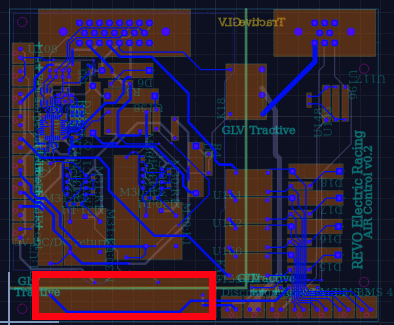
\includegraphics[width = 0.6 \textwidth]{Discharge_PCB}
                \caption{\hlr{The discharge relay is pointed out in the red box, on the PCB containing most of the accumulator wiring (called AIR control board). The resistor will be located right next to the PCB, at the same height of the accumulator.} }
                \label{fig:my_label}
            \end{figure}

    \subsection{HV Disconnect (HVD)} \label{hvdsection}

        \subsubsection{Description}

            We will be using an Anderson Power Products SB Smart VEH-G12 HVD (P/N 115158G12 Vehicle Side and P/N 115158G11 Outboard Side) as our high voltage disconnect, provided by Zero Motorcycles. The part we have in-hand also has a rubber grip on the outboard side of the HVD, which gives the user a greater purchase on the HVD, as shown in Figure \ref{HVDoneside}.

        \subsubsection{Wiring, Cables, Current Calculations, Connectors}

            \begin{figure}[H]
                \centering
                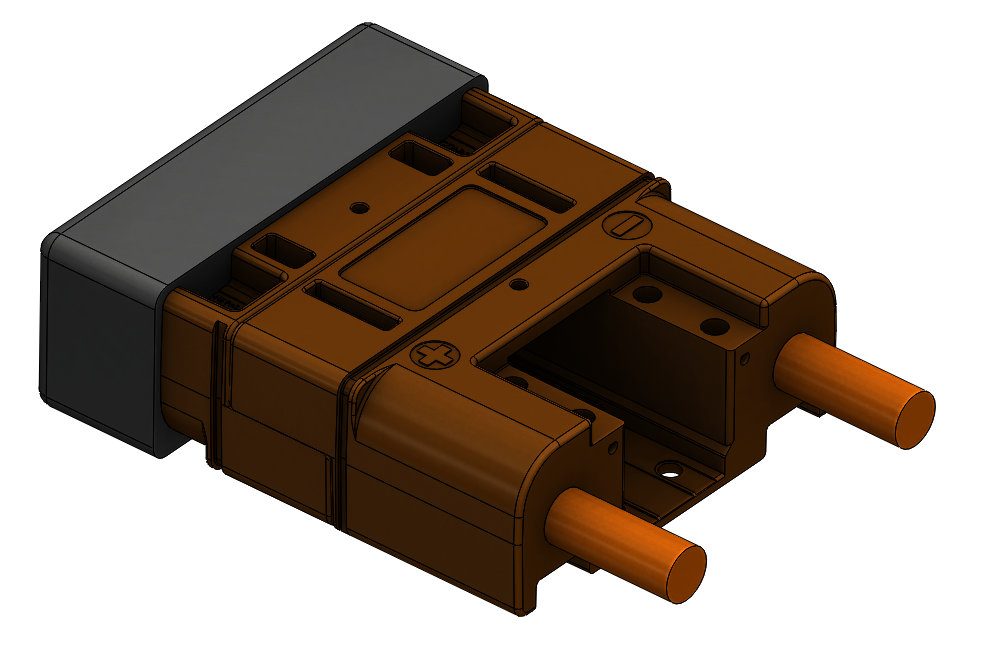
\includegraphics[width = 0.25 \textwidth]{anderson_hvd_interlock}
                \caption{Anderson Power Products SB Smart VEH-G12 HVD}
                \label{HVDoneside}
            \end{figure}

            %Describe wiring, show schematics, describe connectors and cabs and show useful data regarding the wiring.  Include information on the working voltage and current rating of the HVD.

            The connector is rated for 600V and 230.0A on the primary contacts. Because the HVD has an interlock connection with the shutdown circuit, when it is opened it shuts down the TS system by opening the shutdown circuit.

            \begin{figure}[H]
                \centering
                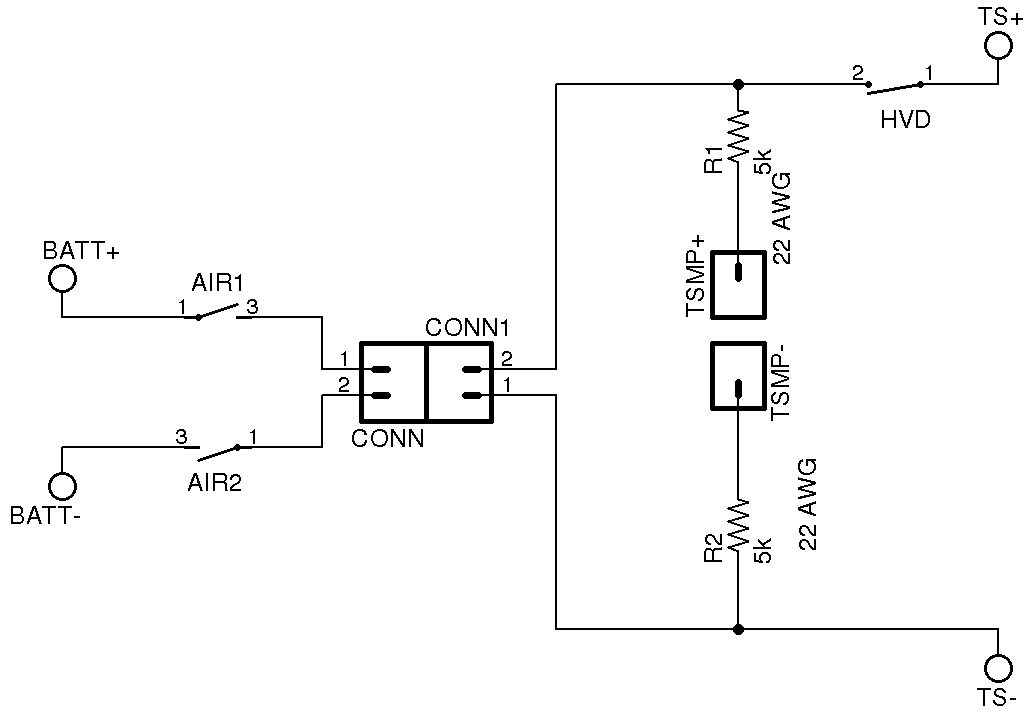
\includegraphics[width = 0.75 \textwidth]{HVD}
                \caption{\hlr{Schematic of primary tractive system connections}}
                \label{HVDschem}
            \end{figure}

        \subsubsection{Position in Car}

            \hlr{The HVD comes out of the accumulator, as it is in-line with the tractive system high side wire. In figure} \ref{hvdlocation}\hlr{, it is the only non-shaded part, with the view being from the back right of the vehicle. The HVD is attached to the motor controller mounting brackets, which are made of 1/8" and 1/16" steel.} The HVD will be clearly indicated and located higher than 350mm from the ground, as per EV 4.7.1.


        \begin{figure}[H]
            \centering
            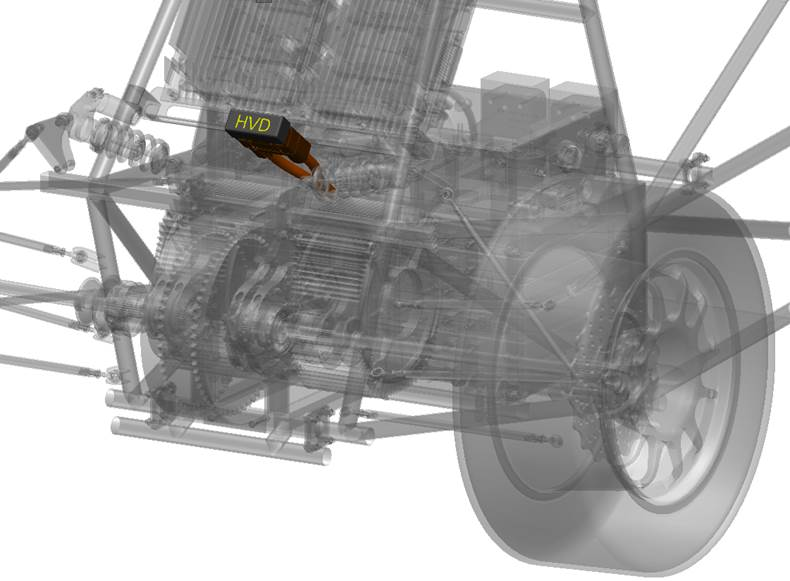
\includegraphics[width = 0.6 \textwidth]{hvd_position}
            \caption{\hlr{Position of the HVD in the vehicle. It is located in line with TS+, and is attached to the motor controller housing in the back of the vehicle. }}
            \label{hvdlocation}
        \end{figure}

    \subsection{Ready To Drive Sound (RTDS)} \label{R2Dsection}

        \subsubsection{Description}

            The Ready to Drive sound includes a buzzer \href{http://www.mallory-sonalert.com/Specifications/SC648ANR.pdf}{\hlr{(Link: Mallory Sonalert Products Inc. SC648ANR)}}, a CAN node, and a relay. The buzzer automatically makes a noise when given power, with the loudness proportional to the voltage. The last step in the startup up sequence will notify the CAN system it is time for the ready to drive sound. Then the corresponding node on the buzzer will close a relay between TS+, after a 2.6 kOhm resistor (5 Watts), and the buzzer for two seconds. The resistor limits the voltage over the buzzer to 48V and the current to 20 mA. \hlr{The SC648ANR is rated to be 95 dB(A) at 2 ft.}

        \subsubsection{Wiring, Cables, Current Calculations, Connectors}

            When the shutdown circuit closes and activates the AIRs \hlr{and the start button has been pushed (while the driver's foot is on the brake),} the car is in ready to drive mode. As soon as the car is in this mode, the CAN system will activate the ready to drive sound node to send a positive output that powers the relay for 2 seconds, thus letting the buzzer sound for 2 seconds. \hlr{This CAN node (called side panel)} is also connected to the IMD, and the full schematic can be found in figure \ref{IMD}. The resistor will be current-limiting and act in the place of a fuse.

                \begin{figure}[H]
                    \centering
                    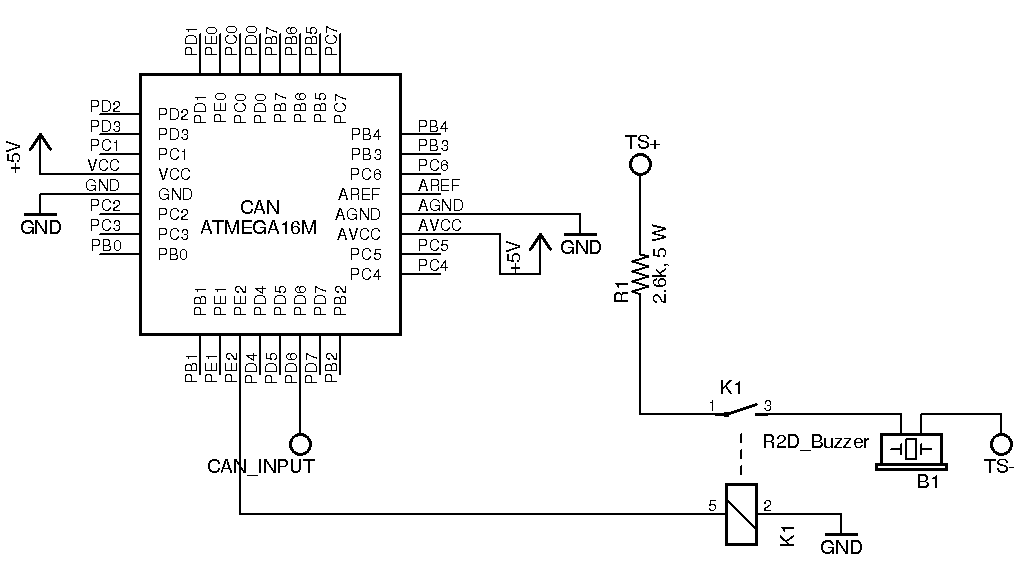
\includegraphics[width = 0.9 \textwidth]{R2Dsoundbuzzerschem}
                    \caption{Schematic for the Ready to Drive Sound Buzzer}
                    \label{R2D}
                \end{figure}

            \begin{align}
                V &= I * R\\
                100-48 V &= 0.021A * R\\
                R &= 2285 \ohm
            \end{align}

            \begin{align}
                P &= I * V \\
                P &= 0.021A * 52 V \\
                P &= 1.09W
            \end{align}

            According to these calculations, a 2.6k$\ohm$ 5W resistor will function as a current limiting resistor.

        \subsubsection{Position in Car}

            The ready to drive sound will be located in the enclosure shown in Figure \ref{cpanel2}. The buzzer will be mounted to the exterior and bottom of this enclosure. \hlr{It must be contained outside of the box so that the buzzer is loud enough}.

\newpage

\section{Accumulator}

    \subsection{Accumulator Pack 1} \label{Battery1}

        \subsubsection{Overview/Description/Parameters} \label{batteryoverview}

            %Describe concept of accumulator pack, provide table with main parameters like number of cells, cell stacks separated by maintenance plugs, cell configuration, resulting voltages->minimum, maximum, nominal, currents, capacity etc.

            The accumulator comprises 12 Nissan Leaf battery modules, wired in series. Each module comprises four LiMnO2 pouch cells, in a 2S-2P configuration as shown in Figure \ref{module}. Each module has a shutdown separator in the middle of each string of cells in parallel (at points MIDPWR1 and MIDPWR2 in section \ref{cellconfiguration}). Each cell has a nominal voltage of 3.75V, resulting in 7.5V per module and 90V total. The modules have alternating positive and negative terminal locations to make bus bar routing more efficient.

            \begin{table}[H]
            \centering
            \begin{tabular}{|l|l|}
            \hline
            Maximum Voltage & 99.6 VDC \\ \hline
            Nominal Voltage & 90 VDC \\ \hline
            Minimum Voltage & 60 VDC \\ \hline
            Maximum output current & Unknown \\ \hline
            Maximum nominal current & \hlr{NDA} \\ \hline
            Maximum charging current & 17 A \\ \hline
            Total number of cells & 48 \\ \hline
            Cell configuration & 12 2s2p in series \\ \hline
            Total capacity & 65 Ah at 2C rate, 25 \degree C \\ \hline
            Number of cell stacks & 4 \\ \hline
            \end{tabular}
            \caption{Main accumulator parameters}
            \label{batterytable}
            \end{table}

            \hlr{The maximum voltage is calculated from the maximum charging voltage, (4.15V per cell), and the maximum charging current is the maximum of the charger.}

            \begin{figure}[H]
                \centering
                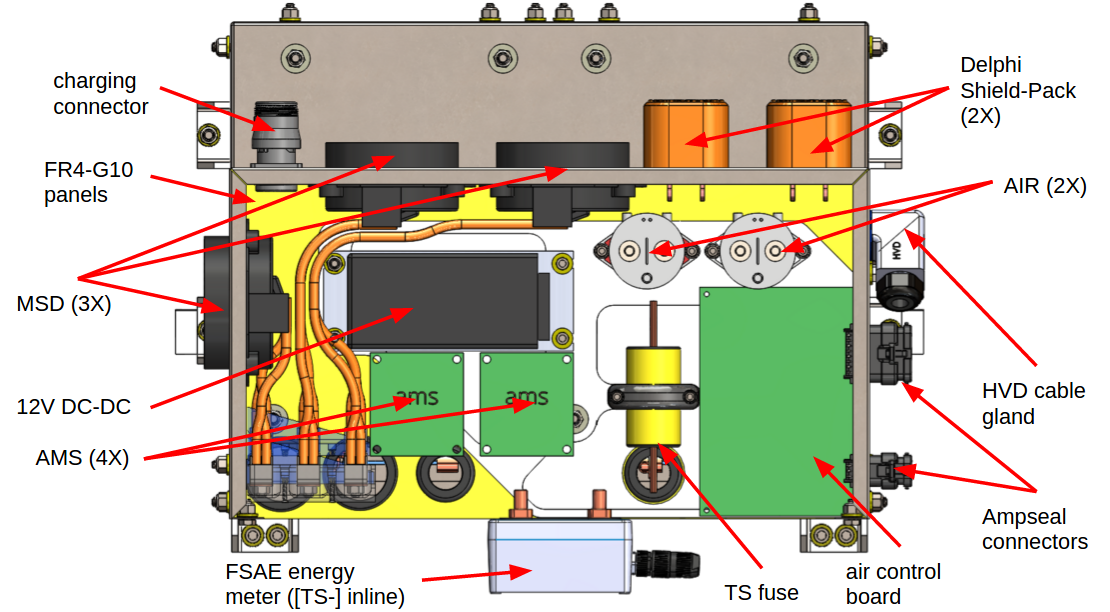
\includegraphics[width = 0.7 \textwidth]{accumulatorlocation}
                \caption{\hlr{Locations of all major parts within the accumulator. }}
                \label{accumlocations}
            \end{figure}

        \subsubsection{Cell Description} \label{celldescription}

            %describe cell type and chemistry
            The cells are laminate type lithium ion cells (LiMnO2), packaged in modules for Nissan Leaf vehicles.

            \begin{table}[H]
            \centering
            \begin{tabular}{|l|l|}
            \hline
            Cell Manufacturer and Type & \begin{tabular}[c]{@{}l@{}}Automotive Energy Supply Corporation\\ Model E5\end{tabular} \\ \hline
            Cell nominal capacity & \hlr{32.2} Ah \\ \hline
            Maximum Voltage & \hlr{4.15V} \\ \hline
            Nominal Voltage & 3.75V \\ \hline
            Minimum Voltage & 2.5V \\ \hline
            Maximum output current & Unknown \\ \hline
            Maximum nominal output current & \hlr{NDA} \\ \hline
            Maximum charging current & \hlr{NDA} \\ \hline
            Maximum Cell Temperature (discharging) & \hlr{NDA, see below} \\ \hline
            Maximum Cell Temperature (charging) & \hlr{NDA, see below}\\ \hline
            Cell Chemistry & \begin{tabular}[c]{@{}l@{}}Lithium-ion - Laminate type\\ Cathode/Anode Material: LIMn2O4 with\\ LiNiO2/Graphite\end{tabular} \\ \hline
            \end{tabular}
            \caption{Main cell specification}
            \label{cells}
            \end{table}

   In software, we are restricting the maximum cell temperature (charging) to 50 \degree C, and the maximum cell temperature (discharging) to 60 \degree C.

        \subsubsection{Cell Configuration} \label{cellconfiguration}

            %Describe cell configuration, cell interconnect, show schematics of electrical configuration and CAD of connection techniques, cover additional parts like internal cell fuses etc.

            \begin{figure}[H]
            \centering
            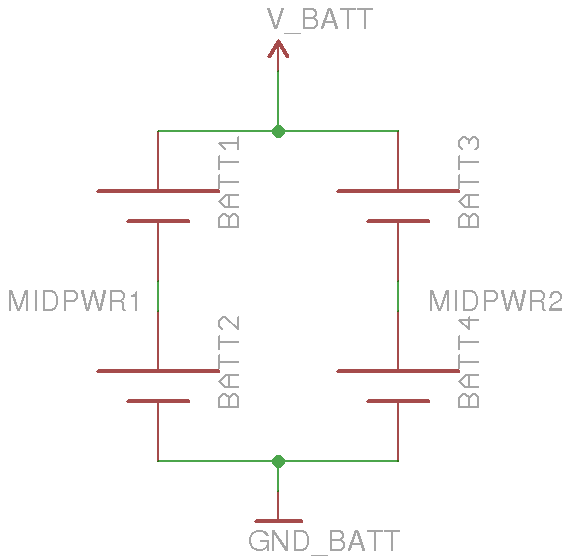
\includegraphics{moduleschem}
            \caption{\hlr{Schematic of a Nissan Leaf Battery Module}}
            \label{module}
            \end{figure}

            As stated in Section \ref{batteryoverview}, there are 12 modules in series. Each module holds 4 cells which are in a 2s-2p configuration. There is a shutdown separator between parallel cells, which acts as a fuse in over-current conditions. The terminal marked in white in Figure \ref{canopener} references the point between the two parallel cell strings. \hlr{The white terminal is the cell interconnection point, as shown in figure} \ref{module}.

            \begin{figure}[H]
            \centering
            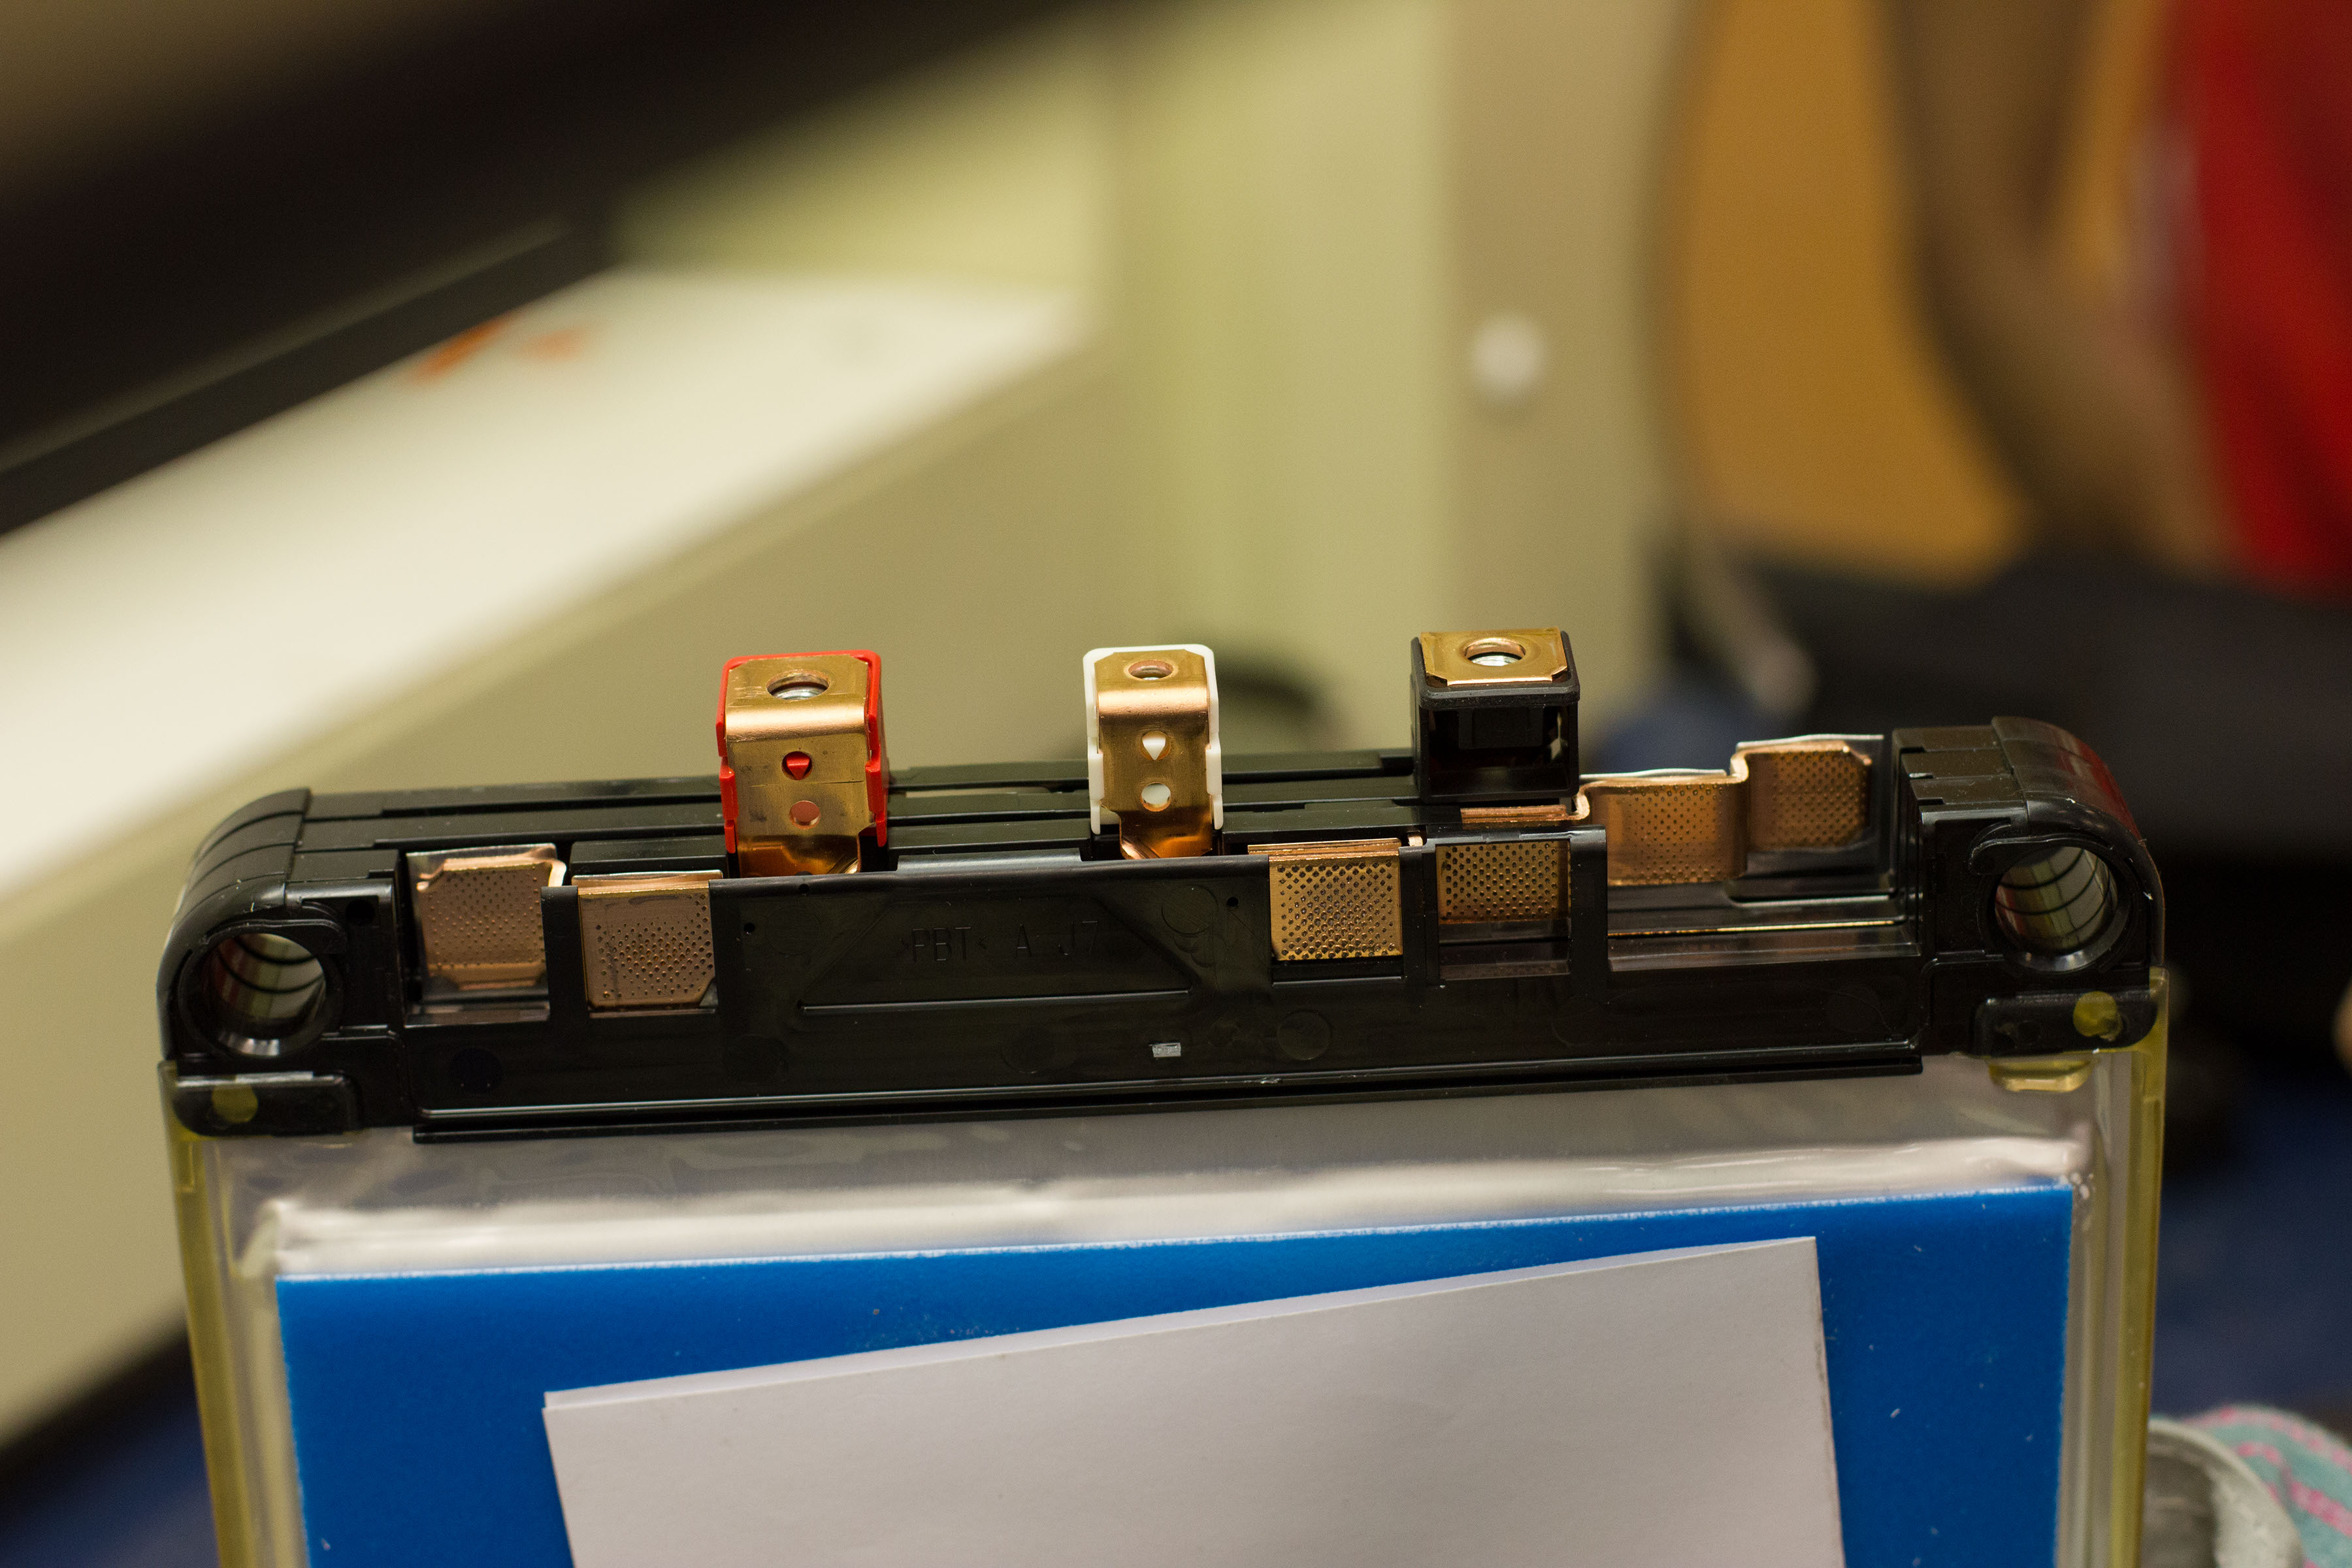
\includegraphics[width = 0.6 \textwidth]{OpenModule}
            \caption{Inside view of a module}
            \label{canopener}
            \end{figure}

            Busbars connect the modules in series, as shown in Figure \ref{busbar}. The busbars connecting module to module are copper with a cross-section of 60.5 mm$^2$, which exceeds the required wire gauge for tractive system lines (2 gauge).

            \begin{figure}[H]
                \centering
                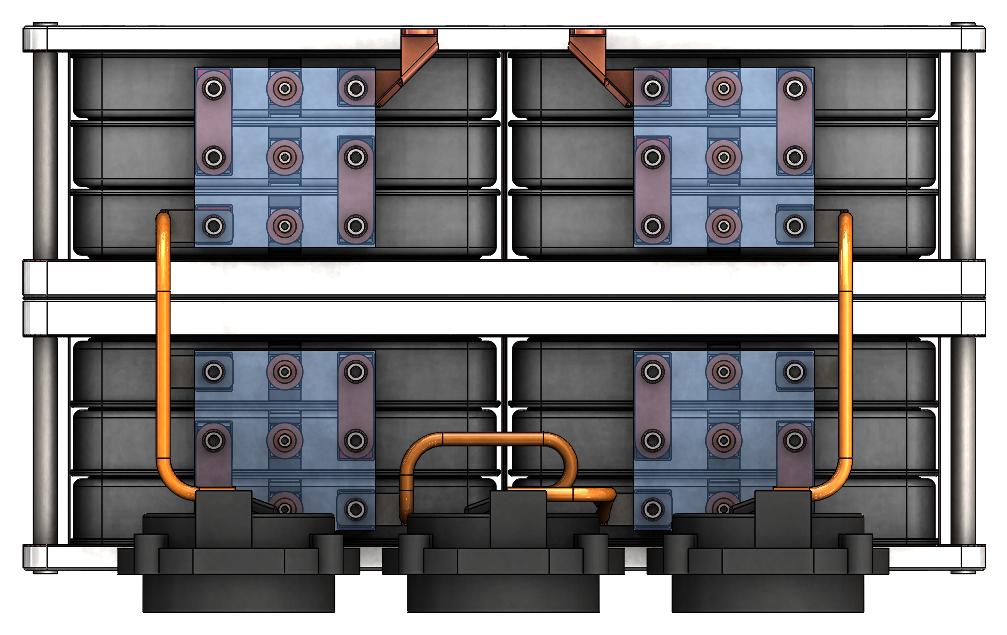
\includegraphics[width = 0.6 \textwidth]{busbar_routing}
                \caption{\hlr{Busbar Routing with MSD Wire Leads}}
                \label{busbar}
            \end{figure}

            \hlr{There are 3 maintenance plugs, separating the segments to be less than 6 MJ each. Figure }\ref{accumlocations} \hlr{ points out the maintenance plugs, shortened as MSD. The connectors are further described in section} \ref{batteryconnectors}.

        \subsubsection{Cell Temperature Monitoring} %\label{celltemp}

            %Describe how the temperature of the cells is monitored, where the temperature sensors are placed, how many cells are monitored, etc. Show schematics, cover additional parts, etc.

            The temperature of the cells is monitored using 10K\ohm thermistors attached to the \hlr{middle pole}. The middle pole of each module is considered the \hlr{negative terminal} of two cells. Each module’s midpoint is measured and one out of three module grounds is measured per accumulator segment. The thermistors are used to form three voltage dividers. When the temperature of the cells increases, the resistance decreases, resulting in less voltage drop across the thermistor. Three analog to digital converters attached to each of the voltage dividers is then used by the ATmega16M1 used in the CAN system to determine whether the temperature is too high or low. If the temperature is out of range, the shutdown system activates. There is a pull up resistor that pushes the output voltage to 5V if the ADC is a past a certain threshold and 0V otherwise. Because we are monitoring the negative terminals of half of the cells in each module, we are monitoring 50\% of the total cells.

            %need to rewrite the part about the ADC
            %How are the thermistors attached to the cells? Explain module issues with placement.


            \begin{figure}[H]
            \centering
            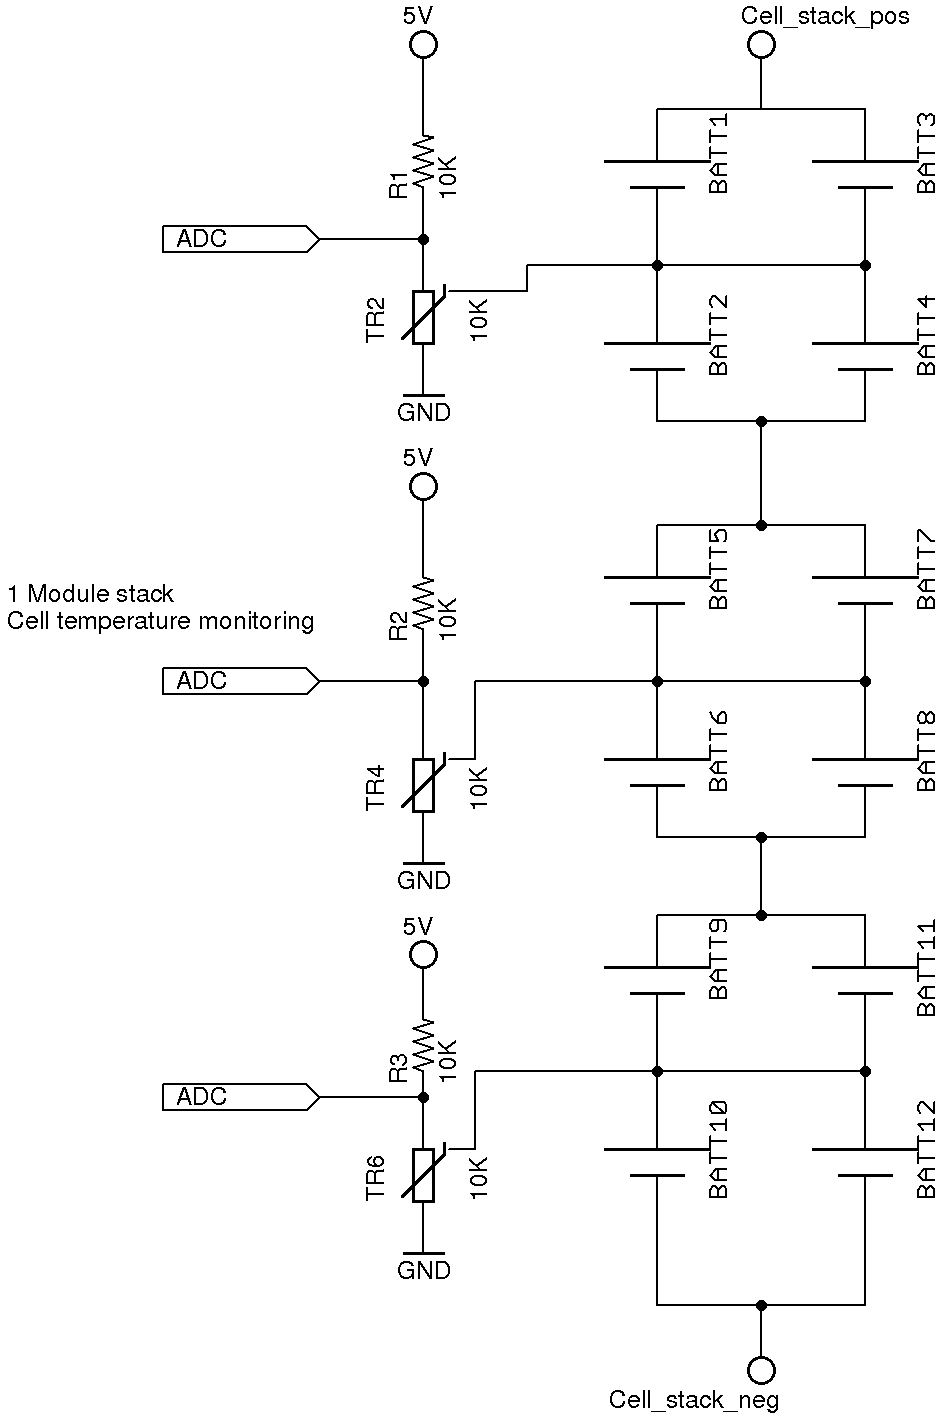
\includegraphics[width = 0.5 \textwidth]{celltemp}
            \caption{Schematic, (1) Module Cell Temperature Monitoring}
            \label{celltemp}
            \end{figure}

        \subsubsection{Battery Management System} \label{bms}

            %Describe how many cells are sensed by each BMS board, the configuration of the cells, the configuration of the boards and how any comms wiring between boards is protected
            %Describe how the BMS is able to open the %AIRs if any error is detected
            %Describe where galvanic isolation occurs between TS and GLV system connections.
            %the configuration of the cells, the configuration of the boards and how any comms wiring between boards is protected

            %Sense wiring protection (fusing / fusible link wire used)
            %What upper and lower voltage does the BMS react at and how does it react?
            %What cell temperature does the BMS react at and how does it react?
            %Show tables of operation parameters

           \hlr{There are 4 AMS modules, and each AMS monitors 6 groups of cells in series}. Each module contains 4 cells, 2 series x 2 parallel, so each AMS monitors 3 modules, or 12 cells (6 series x 2 parallel). There are 4 AMS boards. Each AMS board is coupled to a cell breakout board, which includes 3 thermistors and bolts to the power terminals of three modules, as shown in Figure \ref{busbar} (blue circuit boards). The purpose of the cell breakout boards is to help manage wiring inside the accumulator. The cell breakout boards will have compression limiting copper pads at the terminal bolts and will be spaced above the bus bars using copper washers.\\

            The AMS shunts 3 A when the cell gets above \hlr{4.15 V}. The AMS opens a relay in line with the shutdown circuit if any cell drops below 2.5 V \hlr{or above 4.15V}. The AMS opens a relay in line with the shutdown circuit if any cell gets above 60 \degree C.\\

            \hlr{CAN communication from the board is isolated via a TI ISO1050DUBR (isolated CAN transceiver)}. Only CAN communication is used to have the information from each AMS relayed to the rest of the system, and the boards are otherwise independent of each other. \hlr{Each board has an electrical connection with a normally-open relay on the AIR control board (ie. there are four AMS relays), and the ATmega16M1 of each CAN node can open its relay.} On each cell-top board, there are 7 surface mount Bel C1Q 3A fuses. (Lowest voltage reference and top voltage of each of 6 cells.) The relays which allow the AMS to control the shutdown circuit provide isolation between the AMS and the GLV system, as well as the isolated CAN transceivers. \hlr{Please see Figure} \ref{amsschem} \hlr{for the schematic of one of the battery management system boards.}\\

            %table of operation parameters

            Figure \ref{bmspcb} shows the CAD of one AMS PCB. The AMS boards only communicate through the CAN system. Close ups of this PCB in figure \ref{creepage} show the protective distances between the components of the tractive system and low voltage. Figure \ref{amsschem} in the appendix is to refer to the schematic of the AMS.

            \begin{figure}[H]
                \centering
                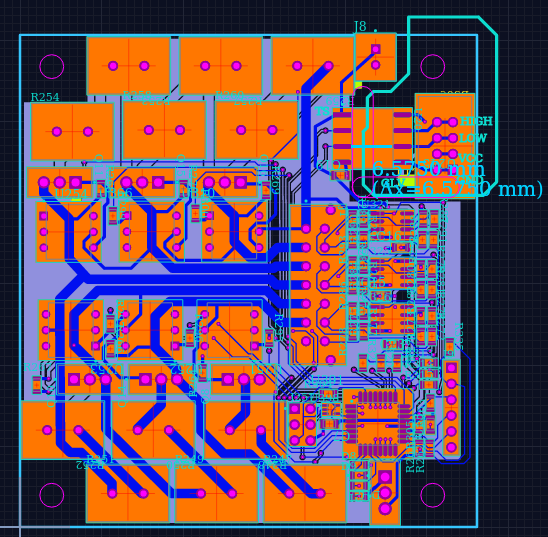
\includegraphics[width = 0.7 \textwidth]{bms_final1_PCBCAD}
                \caption{\hlr{CAD of 1 AMS board (all identical). Cyan polygon indicates GLV voltage, and the $\Delta x$ measurement is the distance between TS and GLV ($6.57$ mm)}.}
                \label{bmspcb}
            \end{figure}


            \begin{figure}[H]
                \centering
                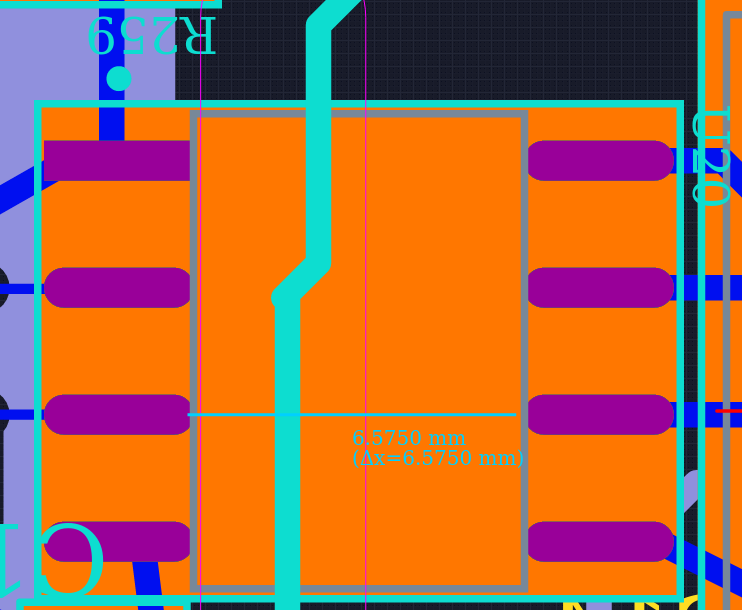
\includegraphics[width=0.5 \textwidth]{bms_separation_detail}
                \caption{\hlr{Detail of BMS PCB where the minimum over surface distance (6.4 mm) are met. Distance between TS and GLV is shown to be $6.57$ mm (over surface)}}
                \label{creepage}
            \end{figure}

            Voltage and temperature data is relayed to the AMS by the cell breakout boards discussed earlier in this section. \hlr{The cell top boards are electrically identical, but have two different layouts to accomodate which side of the accumulator they are on. There is a left hand side, figure} \ref{celltopLH}\hlr{ and right hand side, figure} \ref{celltopRH}. The cell breakout board contains fuses on all sensing lines, detailed in Figures \ref{celltopschem} - \ref{celltopLH}.

            \begin{figure}[H]
                \centering
                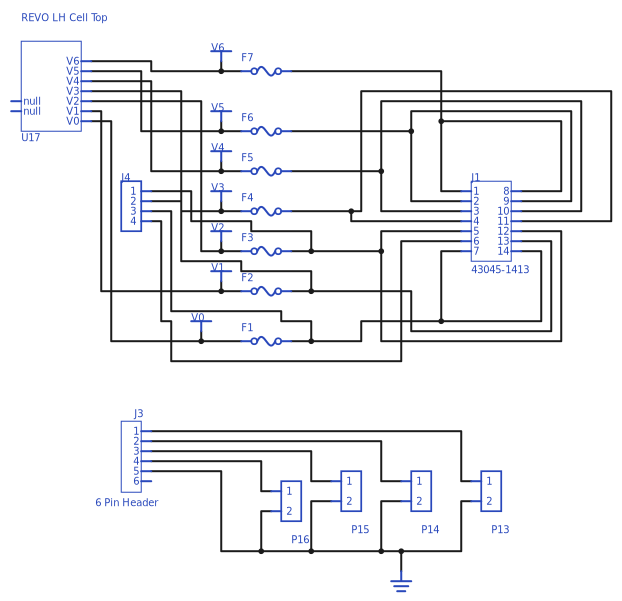
\includegraphics[width = 0.4 \textwidth]{CellTopSchem}
                \caption{Schematic of Cell Breakout Board Connecting to the AMS}
                \label{celltopschem}
            \end{figure}

            %%replace that schematic if you have time, that logo sucks.

            \begin{figure}[H]
                \centering
                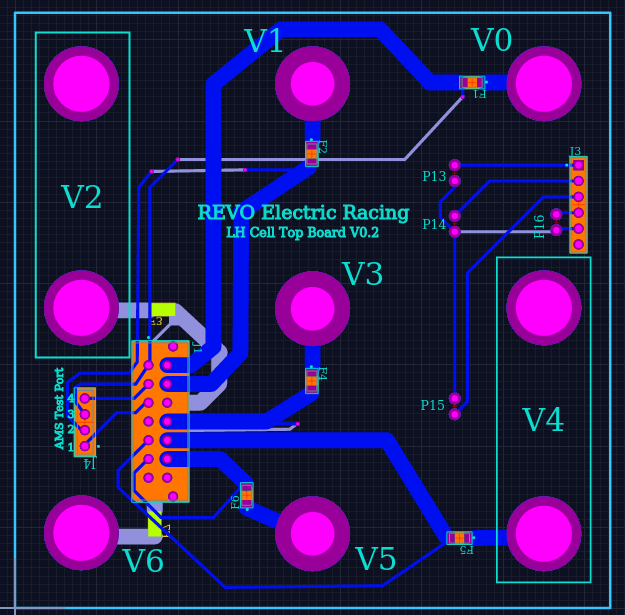
\includegraphics[width = 0.4 \textwidth]{CellTopLH}
                \caption{\hlr{Cell Breakout Board PCB Layout for the left hand side Note the fuses labeled with "F" and then a number. There is only TS voltage on this PCB.}} %The terminals left unconnected will be connecting to the other module stacks, with a fuse in the middle from the segment separator connectors.}
                \label{celltopLH}
            \end{figure}

            \begin{figure}[H]
                \centering
                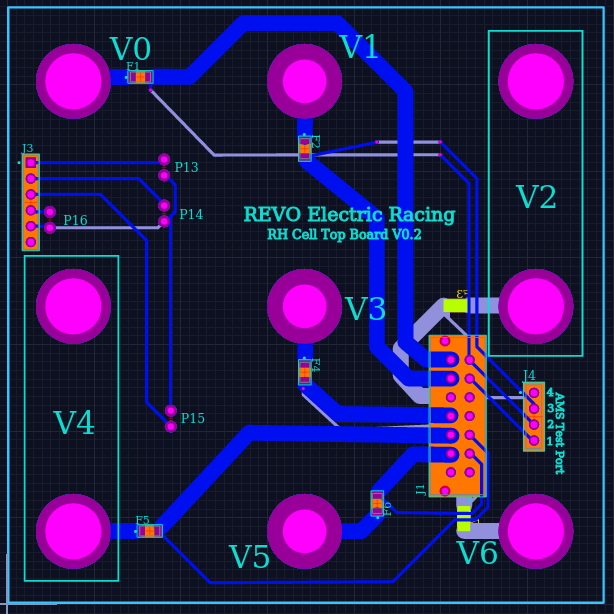
\includegraphics[width = 0.4 \textwidth]{CellTopRH}
                \caption{\hlr{Cell Breakout Board PCB Layout for the right hand side Note the fuses labeled with "F" and then a number. There is only TS voltage on this PCB.}}
                \label{celltopRH}
            \end{figure}
            \hlr{The location of the cell top boards can be seen in figure} \ref{busbar}.

        \subsubsection{Accumulator Indicator} \label{aindicator}
        %doesn't the accumulator indicator need to be run off of AIR control voltage? The pertinent rule is EV 3.3.9. The DC-DC can be powered without the AIR's being %closed.

            %describe the indicator %need table of operation, pcb design, etc.

            \begin{figure}[H]
            \centering
            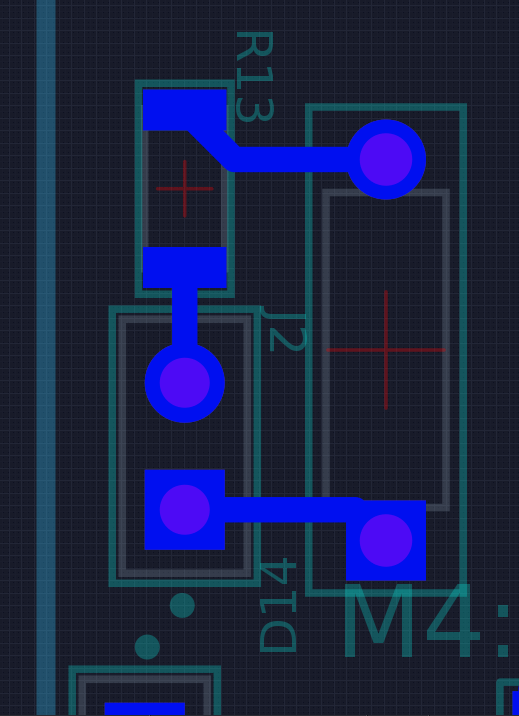
\includegraphics[width = 0.3 \textwidth]{ai}
            \caption{Detail of the Accumulator Indicator PCB}
            \label{indicator}
            \end{figure}

            As shown in Figure \ref{indicator}, J2 connects the accumulator indicator, D14, \hlr{to a zener diode running of TS voltage. The zener diode allows TS voltage to pass through the accumulator indicator LED and a resistor (to limit current)} after TS voltage is over 60 VDC. \hlr{The accumulator indicator is located on the AIR control board PCB, and has traces of 20 mil, which are rated for 1.4A, while the maximum current (using the current limiting resistor) will be 45mA. }

        \subsubsection{Wiring, Cables, Current Calculations, Connectors} \label{batteryconnectors}

            \hlr{There are 4 cells (in a 2s2p configuration) in each module, and there are 12 modules in series. The accumulator has them separated into 4 stacks of 3 to comply with the segment energy limit. Between each of the segments, there are MSDs for safely separating the segments while working on the accumulator. After the fourth section, there is an HVD in series with the positive pole, coming out of the accumulator. There will be two main connectors to the accumulator, each having connections of TS+ and TS-. This is so each motor controller can be individually connected to. Before the HVD and main connectors, there is an AIR on both the positive and negative poles of TS. }

            The high current (motor, motor controller) wires used for the tractive system will be as described in table \ref{motorwire}.
            The low current (IMD, Lights DC-DC, GLV DC-DC and ready to drive sound) TS connections will be made with the wire described in table \ref{tslowcurrentwire}.

            \begin{table}[H]
            \centering
            \begin{tabular}{|l|l|}
            \hline
            Wire type & \hlr{CnC Tech}, 22 AWG \\ \hline
            Current rating & 7A \\ \hline
            Cross sectional area & 0.326 mm\textasciicircum 2 \\ \hline
            Maximum voltage & 600V \\ \hline
            Temperature rating & 120 \degree C \\ \hline
            \begin{tabular}[c]{@{}l@{}}Wire connects the\\ following components:\end{tabular} & \begin{tabular}[c]{@{}l@{}}TS V to GLV DC-DC converter, \\ TS V to IMD HV input, \\ TS V to ready to drive sound buzzer\end{tabular} \\ \hline
            \end{tabular}
            \caption{Wire data of the company: CnC Tech, 0.326 mm$^{2}$}
            \label{tslowcurrentwire}
            \end{table}

            %ADD 18 AWG wire for IMD's connectors

            % Describe your maintenance plugs, provide pictures
            We will use OEM maintenance plugs provided by General Motors. As shown in Figure \ref{msd03}, these maintenance plugs, known internally as Manual Service Disconnects (MSD's), comprise a panel-mounted plastic housing (black) and a plastic plug (orange). The plug must be twisted and then pulled in two distinct steps, which disengages the copper bus-bar, contained in the orange plug, from spring-loaded contacts contained in the black housing. \hlr{There will not be any fuses in the MSDs.} General Motors will also be crimping custom length leads onto these MSD's for our vehicle. The leads are 40 mm$^2$ in cross-section, not including insulation. Each MSD also contains a two-pin interlock, as described in Section \ref{interlocks}. To the best of our knowledge, these MSD's comply with EV 3.3.3. Additionally, the spring-loaded contacts located in the black housing are encapsulated in plastic, providing protection from shorting and accidental contact.


            \begin{figure}[H]
                \centering
                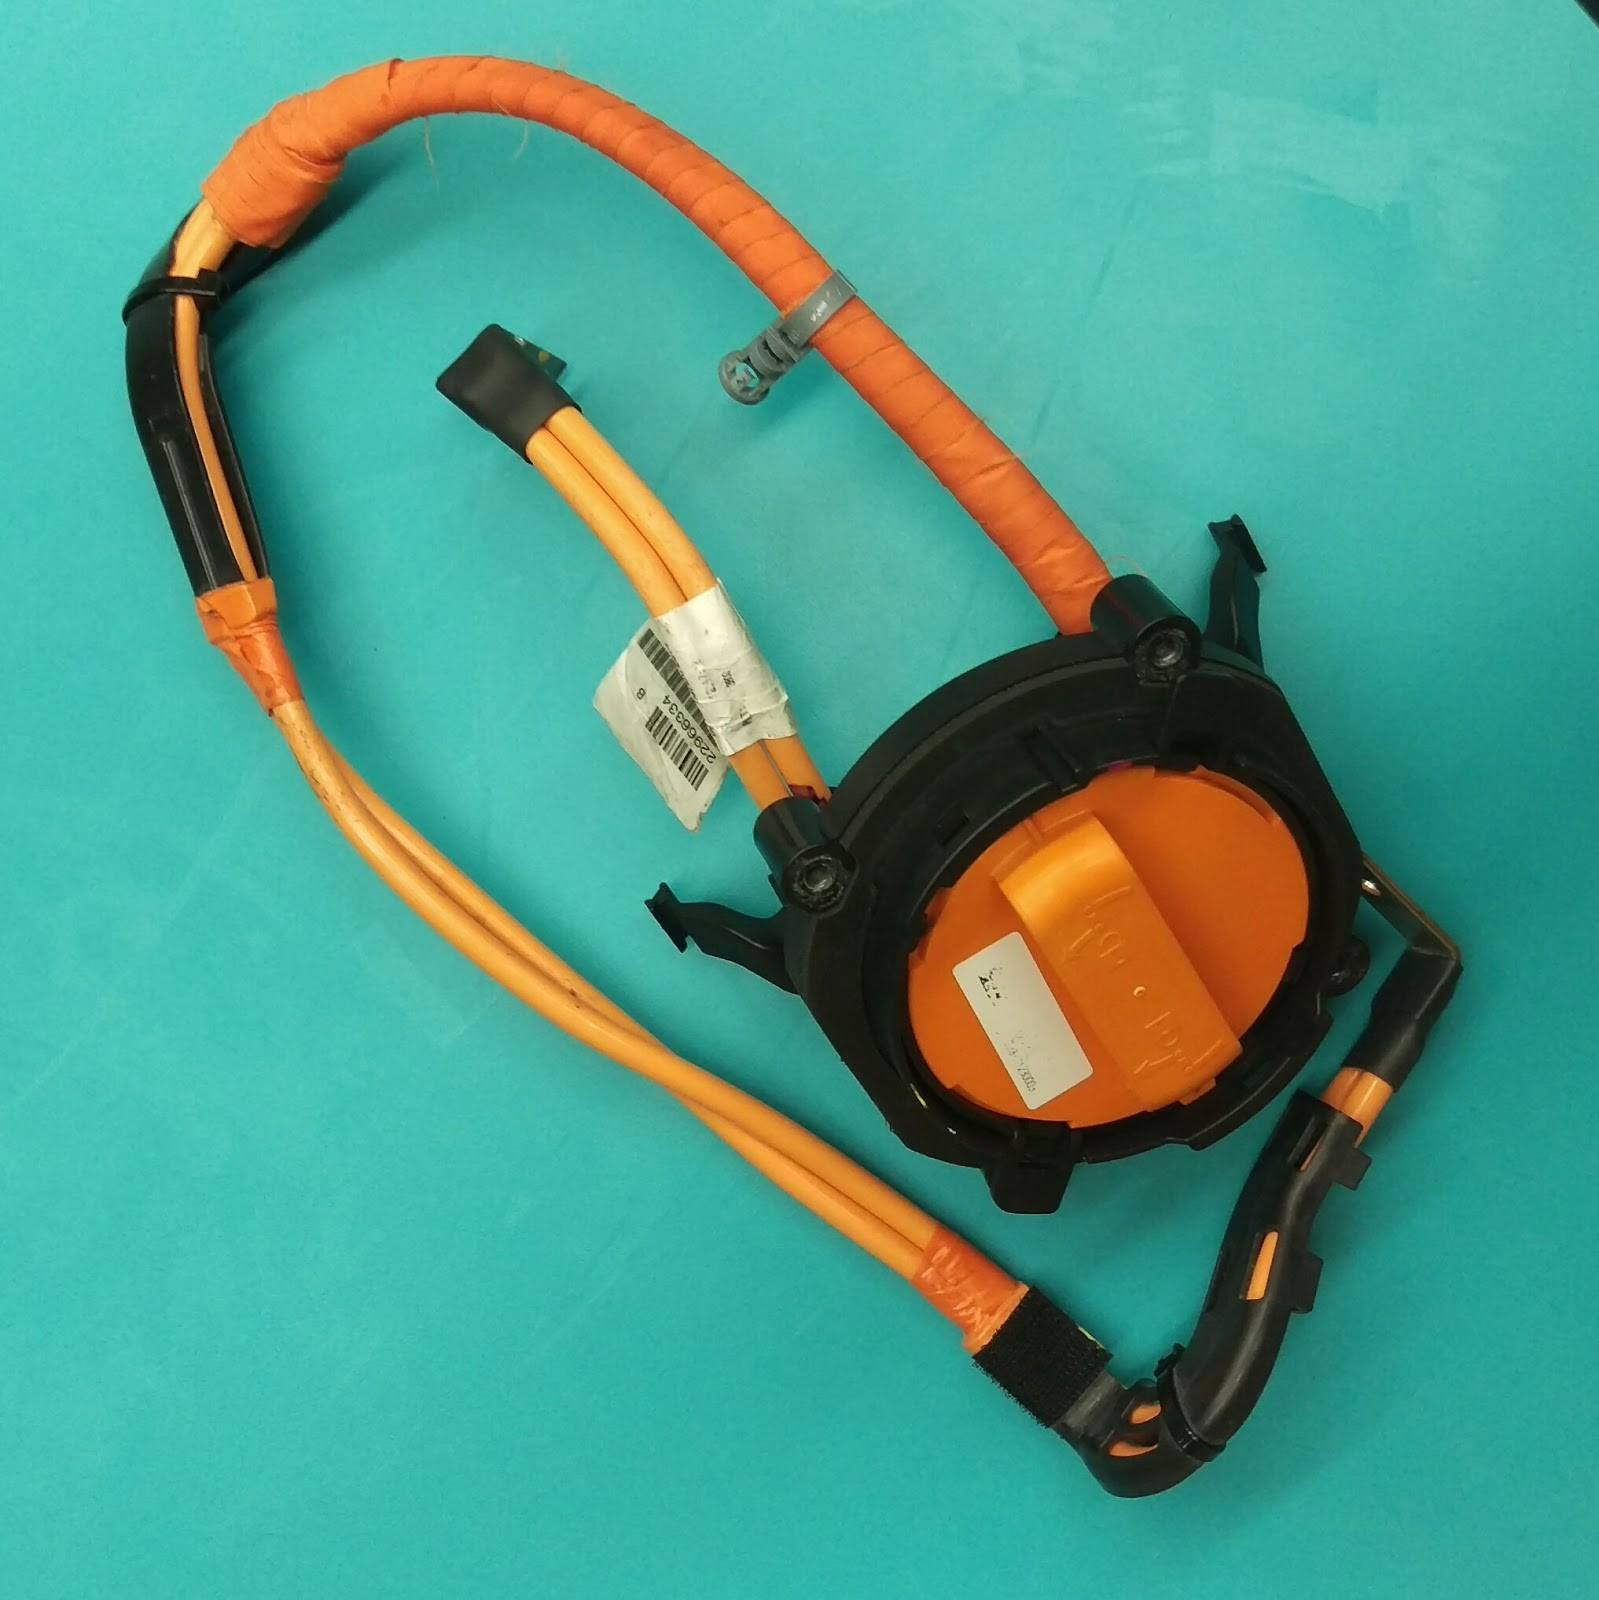
\includegraphics[width = 0.5 \textwidth]{msd_highres}
                \caption{Manual Service Disconnect (Maintenance Plug)}
                \label{msd03}
            \end{figure}

        \subsubsection{Accumulator Insulation Relays (AIR)} \label{airs}

            %Describe the AIRs

            We will use Kilovac EV200 relays as accumulator insulation relays. They will be paired with economizer circuits to draw less current during normal usage. The relay requires a 12 V control signal, and is rated for 500 A. Figure \ref{prechargeschem} shows the schematic location of the economizers and the AIR's.

            \begin{table}[H]
            \centering
            \begin{tabular}{|l|l|}
            \hline
            Relay Type: & Normally Open \\ \hline
            Contact arrangement & SPST-NO-DM \\ \hline
            Continuous DC current rating & 500A \\ \hline
            Overload DC current rating & 2000A \\ \hline
            Maximum operation voltage & 900VDC \\ \hline
            Nominal coil voltage & 12VDC \\ \hline
            Normal Load switching & See figure \\ \hline
            Maximum Load switching & See figure \\ \hline
            \end{tabular}
            \caption{Basic AIR Data}
            \label{air}
            \end{table}

            \begin{figure}[H]
            \centering
            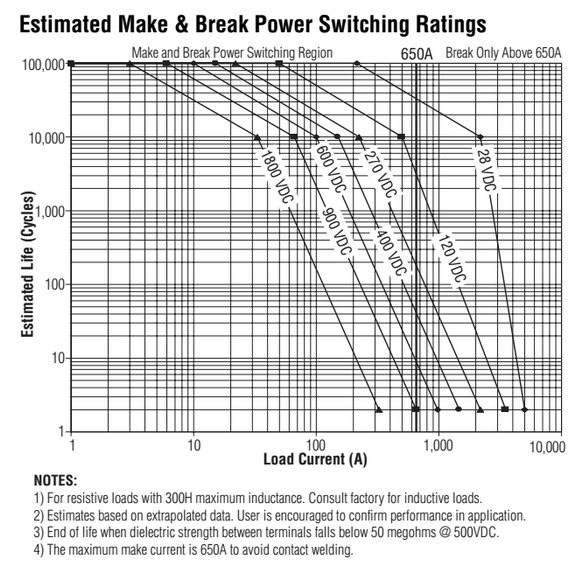
\includegraphics[width = 0.7 \textwidth]{AIRswitching}
            \caption{Load Switching detail from Accumulator Indicator Relay datasheet}
            \label{airswitch}
            \end{figure}

        \subsubsection{Fusing} \label{fusing}

            %Describe the fuses used and their main operation parameters, use tables, etc.

            \begin{table}[H]
            \centering
            \begin{tabular}{|l|l|}
            \hline
            Fuse manufacturer and type: & \hlr{Littledfuse, SPF Series (SPF-004)} \\ \hline
            Continuous current rating & 4A \\ \hline
            Maximum operating voltage & 1000 V \\ \hline
            Type of fuse & Fast acting \\ \hline
            I2t rating & @10kA: 76.270, @20kA: 80.254 \\ \hline
            \begin{tabular}[c]{@{}l@{}}Interrupt Current (max. current\\ at which the fuse can interrupt\\ the circuit)\end{tabular} & $20$ kA \\ \hline
            \end{tabular}
            \caption{GLV fuse,  type}
            \label{glvfusetable}
            \end{table}

            \begin{table}[H]
            \centering
            \begin{tabular}{|l|l|}
            \hline
            Fuse manufacturer and type: & \hlr{Littledfuse, MINI Series (MIN2BP)} \\ \hline
            Continuous current rating & \hlr{2}A \\ \hline
            Maximum operating voltage & \hlr{32} V \\ \hline
            Type of fuse & Fast acting \\ \hline
            I2t rating & \hlr{2.8 A2s} \\ \hline
            \begin{tabular}[c]{@{}l@{}}Interrupt Current (max. current\\ at which the fuse can interrupt\\ the circuit)\end{tabular} & \hlr{$1000$A at $32$ VDC}\\ \hline
            \end{tabular}
            \caption{GLV 12V fuse, MIN type}
            \label{glv12vfusetable}
            \end{table}

            \begin{table}[H]
            \centering
            \begin{tabular}{|l|l|}
            \hline
            Fuse manufacturer and type: & \hlr{Littelfuse, MINI Series (MIN2BP)} \\ \hline
            Continuous current rating & \hlr{2}A \\ \hline
            Maximum operating voltage & \hlr{32} V \\ \hline
            Type of fuse & Fast acting \\ \hline
            I2t rating & \hlr{2.8 A2s} \\ \hline
            \begin{tabular}[c]{@{}l@{}}Interrupt Current (max. current\\ at which the fuse can interrupt\\ the circuit)\end{tabular} & \hlr{$1000$A at $32$ VDC}\\ \hline
            \end{tabular}
            \caption{Shutdown system fuse, MIN type}
            \label{shutdownfusetable}
            \end{table}

            \begin{table}[H]
            \centering
            \begin{tabular}{|l|l|}
            \hline
            Fuse manufacturer and type & \hlr{Littelfuse, 251/253 Series} \\ \hline
            Continuous current rating & 1 A \\ \hline
            Maximum operating voltage & 125V \\ \hline
            Type of fuse & Fast acting \\ \hline
            I2T rating &  \hlr{0.405 A2s} \\ \hline
            \begin{tabular}[c]{@{}l@{}}Interrupt Current (max.,current\\ at which the fuse can interrupt\\ the circuit)\end{tabular} & \hlr{$300$A at $125$VDC} \\ \hline
            \end{tabular}
            \caption{\hlr{Fuse to the IMD, TSMPs and light DC-DC converter, 251/253 Series}}
            \label{smallTSfusetable}
            \end{table}

            \begin{table}[H]
            \centering
            \begin{tabular}{|l|l|}
            \hline
            Fuse manufacturer and type & Ferraz Shawmut, Semiconductor AC series (A15QS)\\ \hline
            Continuous current rating & 7A \\ \hline
            Maximum operating voltage & 150VDC \\ \hline
            Type of fuse & Fast acting \\ \hline
            I2T rating & 0.011 at 150 VDC and 10ms \\ \hline
            \begin{tabular}[c]{@{}l@{}}Interrupt Current (max.,current\\ at which the fuse can interrupt\\ the circuit)\end{tabular} & 100kA \\ \hline
            \end{tabular}
            \caption{Fuse to the keyswitch v+}
            \label{keyswitchfusetable}
            \end{table}


            \begin{table}[H]
            \centering
            \begin{tabular}{|l|l|}
            \hline
            Fuse manufacturer and type: & \begin{tabular}[c]{@{}l@{}}Bussmann,\\ LPJ type\end{tabular} \\ \hline
            Continuous current rating & 175A \\ \hline
            Maximum operating voltage & 600 V \\ \hline
            Type of fuse & Time delay \\ \hline
            I2t rating & None listed, see figure \ref{TSi2t} \\ \hline
            \begin{tabular}[c]{@{}l@{}}Interrupt Current (max. current\\ at which the fuse can interrupt\\ the circuit)\end{tabular} & 300 kA \\ \hline
            \end{tabular}
            \caption{Tractive system main fuse, LPJ  type}
            \label{tsfuse}
            \end{table}

            \begin{figure}[H]
                \centering
                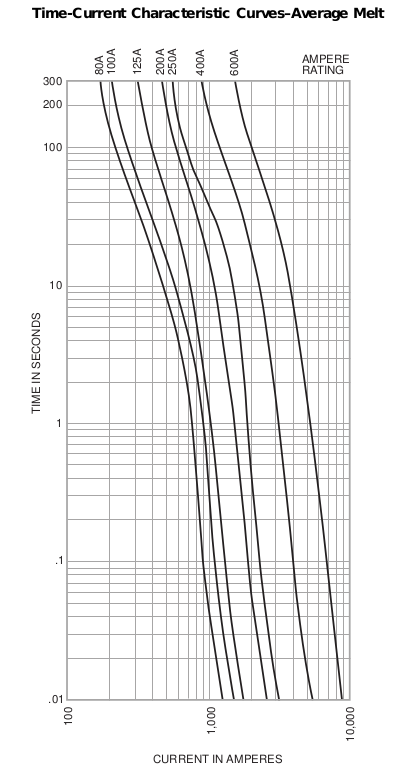
\includegraphics[width = 0.25 \textheight]{TSfuseT-Agraph}
                \caption{TS main fuse (175A) Time-Current information}
                \label{TSi2t}
            \end{figure}

            %Create a table with components and wires protected by the fuse(s) and the according continuous current rating, below is an example table with some potential entries.  Complete this table with information for your design and add/remove additional locations as applicable.  Ensure that the rating of all of the components is greater than the rating of the fuse such that none of the other components become the fuse.

            All wire ampacity ratings are according to the Power Stream's Wire Gauge chart, located in the appendix, Figure \ref{AWGchart}.

            \begin{table}[H]
            \centering
            \begin{tabular}{|l|l|l|l|l|}
            \hline
            Location & Wire Size & Wire Ampacity & Fuse type & Fuse rating \\ \hline
            \begin{tabular}[c]{@{}l@{}}TS Main fuse (before HVD,\\ on pos pole)\end{tabular} & 2 AWG & 181A & LPJ type & 175A \\ \hline
            TS+ to GLV DC-DC converter & 22 AWG & 7A & SPF fuse & 4A \\ \hline
            GLV 12V+ & 22 AWG & 7A & MIN fuse & 2A \\ \hline
            Shutdown pos pole & 22 AWG & 7A & MIN fuse & 2A \\ \hline
            \begin{tabular}[c]{@{}l@{}}TS+ to IMD, TSMPs TSAL's DC-DC\\ converter\end{tabular} & 22 AWG & 7A & ABC fuse & 1A \\ \hline
            \begin{tabular}[c]{@{}l@{}}GLV 12V to 5V regulator \\ (CAN system)\end{tabular} & 22 AWG & 7A & ABC fuse & 1A \\ \hline
            \begin{tabular}[c]{@{}l@{}}Keyswitch, in parallel with\\ TS voltage\end{tabular} & 18 AWG & 16A & AC fuse & 7A \\ \hline
            Cell to BMS x28 & \begin{tabular}[c]{@{}l@{}}PCB\\          trace\end{tabular} & \begin{tabular}[c]{@{}l@{}}Trace\\             ampacity: 7.6 A \\ (open air)\end{tabular} & \begin{tabular}[c]{@{}l@{}}CIQ\\           Fuse x28\end{tabular} & 3A \\ \hline
            \end{tabular}
            \caption{Fuse Protection Table}
            \label{allfuses}
            \end{table}

        \subsubsection{Charging} \label{charging}

            %Describe how the accumulator will be charged. How will the charger be connected? How will the accumulator be supervised during charging? Show schematics, CAD-Renderings, etc., if needed

            \begin{table}[H]
            \centering
            \begin{tabular}{|l|l|}
            \hline
            Charger Type: & Delta Q Technologies QioQ 1000 Series \\ \hline
            Maximum charging power & 70.55 W \\ \hline
            Maximum charging voltage & 4.15V \\ \hline
            Maximum charging current & 17.0A \\ \hline
            Interface with accumulator & CAN-Bus \\ \hline
            Input voltage & 125VAC or 250VAC \\ \hline
            Input current & 13A@125VAC or 10A@250VAC \\ \hline
            \end{tabular}
            \caption{General Charger data}
            \label{charger}
            \end{table}

            This UL-listed charger supplies constant current at 17.0A until cell voltages reach 4.15V. Then, constant voltage is supplied at 4.15 V \hlr{per cell, summing to 99.6V,} until the current tapers to 2.0 A.\\

            The charger will indicate complete on its LED display when the battery voltage reaches \hlr{4.15}V per cell, however it will continue charging until it finishes both stages.\\

            The accumulator will only be charged on the charging cart. This cart has not yet been specified or designed. It will be able to support the full weight of the accumulator and only move when a dead man's switch is activated.\\

            The accumulator cart will contain a specialized shutdown circuit that allows the accumulator to be charged through \hlr{the charging connector, and the shutdown circuit to close without the main accumulator connector interlocks engaged}. The AMS will be active during charging and have the ability to open the AIRs and stop charging in the event of dangerous battery conditions. This shut down circuit will contain a separate IMD, an emergency stop, and an interlocking connection between the charger and accumulator. \hlr{ The separate IMD used is also the IR155-3204 from Bender, the same model of IMD used on the car.}

            \hlr{The connectors used for charging will be the Molex Two-Pin Connector (interlock), integrated with Delphi Shield-Pack (see the next section for details).}


            \begin{figure}[H]
                \centering
                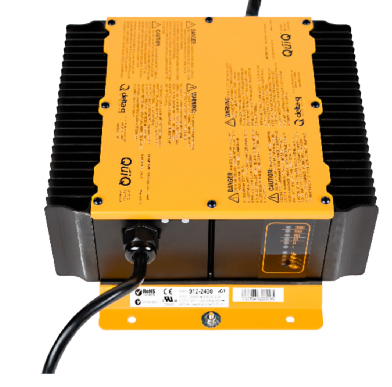
\includegraphics[width = 0.5 \textwidth]{chargepic}
                \caption{DeltaQ 96V QUIQ ICON charger}
                \label{chargepic}
            \end{figure}

        \subsubsection{Mechanical Configuration/Materials}

            %how cells are mounted, data on materials used, and concept of the container

            The accumulator mechanical configuration presented in this document was designed under the assumption that the Nissan module casings were not electrically isolated from the cells. However, after tearing down a module, we found that the casing is completely insulated from the cells and therefore, the design of the accumulator is likely to change.\\

            As shown in Figure \ref{accframe}, the accumulator frame comprises a 1/8" thick welded angle iron frame with panels meeting the minimum material requirement given in EV 3.4.6. Figure \ref{cellexp} shows an exploded view of a half-pack: six cells bolted into 3/4" polycarbonate brackets with 5/16" bolts. Two half-packs slide into the accumulator frame and are bolted into the frame with 5/16" SAE Grade 8 threaded rod and locknuts. Figure \ref{cellcut} shows a cutaway of the bolt stackup for the two half-packs. 4130 steel sleeves limit the compression of the threaded rods bolting the entire pack together. Finite element analysis allowed us to prove structural integrity in 20G vertical and 40G lateral load conditions.

            \begin{figure}[H]
                \centering
                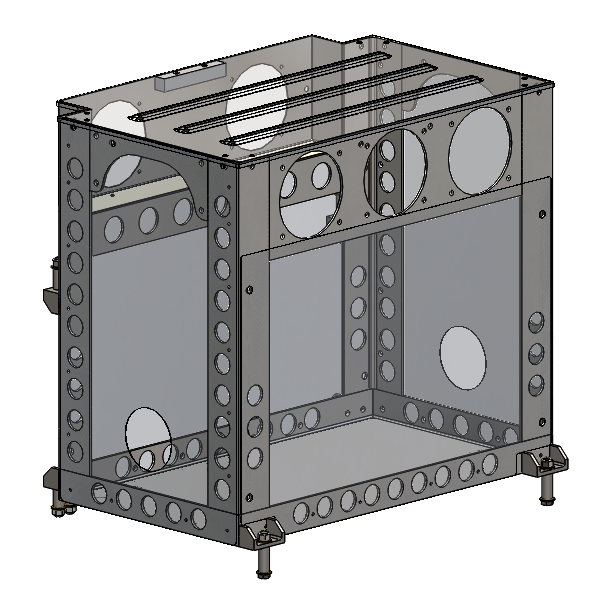
\includegraphics[width = 0.5 \textwidth]{accumulator_frame}
                \caption{Accumulator Frame}
                \label{accframe}
            \end{figure}

            \begin{figure}[H]
                \centering
                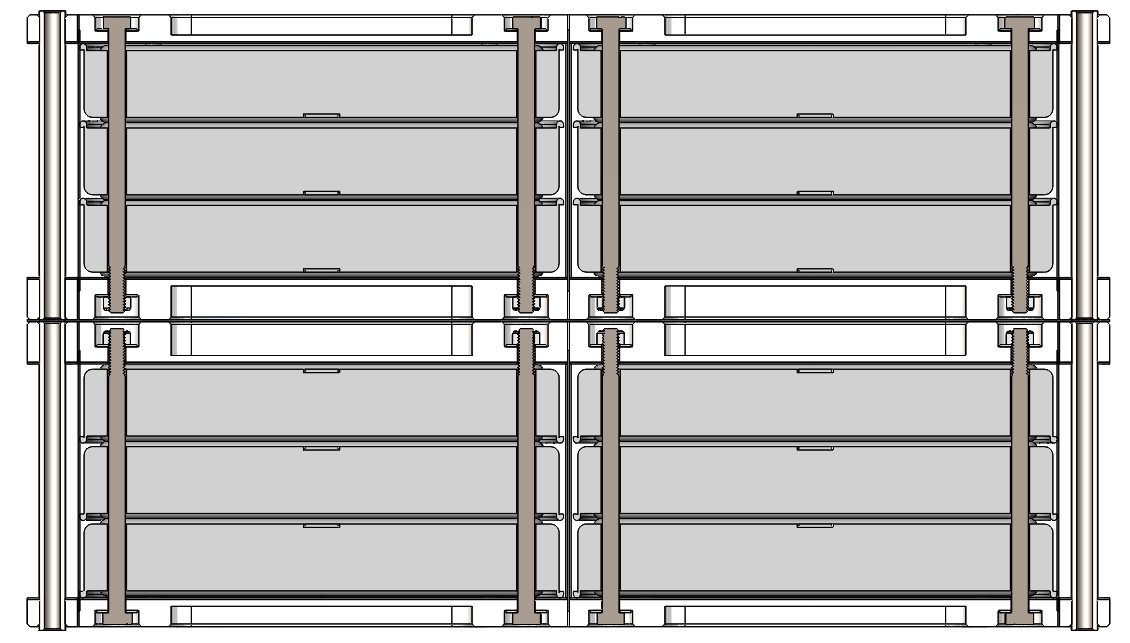
\includegraphics[width = 0.5 \textwidth]{cellmount_cutaway}
                \caption{Cell Mounting Cutaway}
                \label{cellcut}
            \end{figure}

            \begin{figure}[H]
                \centering
                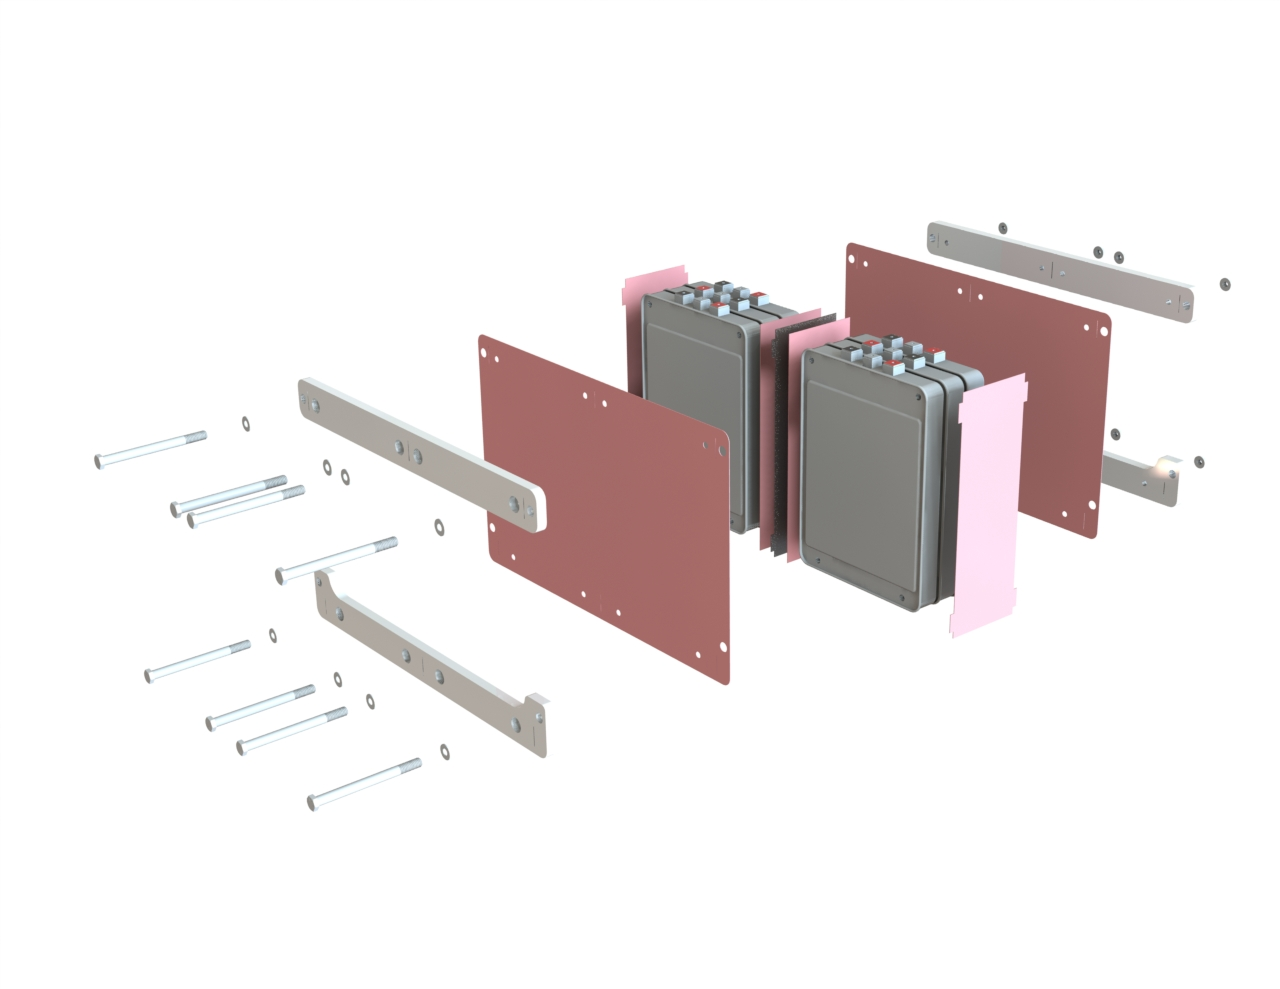
\includegraphics[width = 0.5 \textwidth]{cellmount_exploded}
                \caption{Cell Mounting Exploded}
                \label{cellexp}
            \end{figure}

            \hlr{The connectors used will be:}
            \hlr{Accumulator to MC Connections}
            \hlr{Delphi Shield-Pack HV2000 Connectors}

            \hlr{Accumulator to HVD:}
            \hlr{Hardwired, double-shielded $35mm^2$ stranded wire}

            \hlr{Charging Connector:}
            \hlr{Deutsch HD10 6-Pin (P/N: HD10-6-12P, HD16-6-12S)}

            \hlr{GLVS Connector:}
            \hlr{AMPSEAL 23-Pin, (P/N: 770680-4, 776087-1)}

            \hlr{TS Low-Current Connector:}
            \hlr{AMPSEAL 8-Pin (P/N: 776286-1, 776280-1)}

        \subsubsection{Position in Car}

        The accumulator is located behind the driver, under the main roll hoop, and is entirely encapsulated by the primary frame structure.

    \subsection{Accumulator Pack 2}
        There will only be one accumulator for the vehicle, as described in Section \ref{Battery1}

\newpage

\section{Energy Meter Mounting}

    \subsection{Description}

        %The Energy Meter will be supplied and it will be mounted during E-Scrutineering. It is intended to use the Energy Meter of Formula Student Germany. The current version of the 2012 EM specification can be found here: https://www.formulastudent.de/uploads/media/FSE2012_Energy_Meter_Specification_v1.0.pdf Please note that the connectors might change slightly for 2013.

        The energy meter is a tool made by FSAE to calculate energy use during competition. The meter checks that the voltage is within the rule's ranges, the total power used is not over the maximum limit of 80 kW, and calculates the amount of energy used. The energy is calculated as the time integrated value of the measured voltage multiplied by the measured current logged by the Energy Meter, as per rule EV 4.9.

    \subsection{Wiring, Cables, Current Calculations, Connectors}

        %Describe the wiring, show schematics, provide calculations for currents and voltages, and show data regarding the cables and connectors used.

        The energy meter will measure current in the tractive system by being connected in series with the HV- line. It measures voltage in the system with a connection to HV+. The low power data collection systems inside of the Energy Meter are powered using the GLVS.

    \subsection{Position in Car}

        The energy meter will be integrated with the junction box described in Section \ref{hvdsection}. This is an ideal location for the energy meter because it can be securely mounted in a waterproof location and is proximal to all of the necessary connections.

\newpage

\section{Motor Controller} \label{MCs}

    \subsection{Motor Controller 1} \label{MC1}

        \subsubsection{Description, Type, Operation Parameters}

            %Describe important functions; provide table with main parameters like resulting voltages->minimum, maximum, nominal, currents etc.

            \begin{figure}[H]
                \centering
                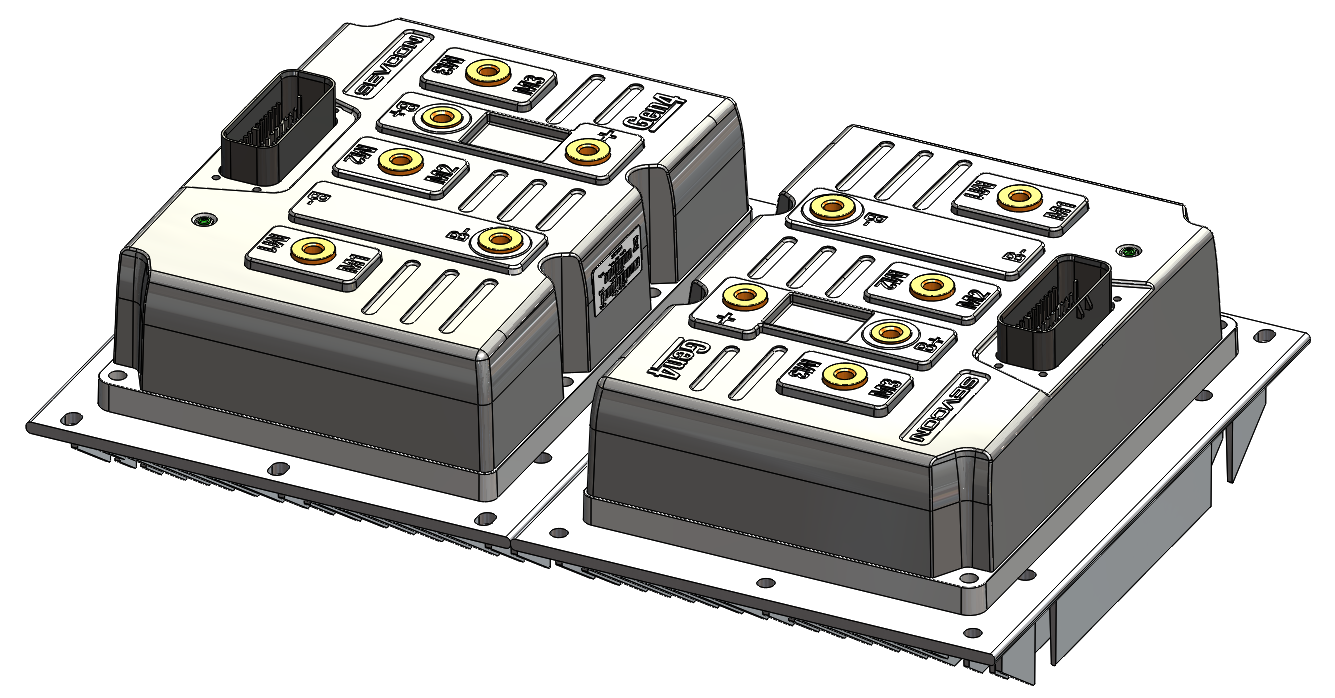
\includegraphics[width = 0.7 \textwidth]{motorcontrollers_separate}
                \caption{Sevcon Gen 4 Size 4 motor controllers}
                \label{mcoffcar}
            \end{figure}

            \hlr{The two motor controllers used are both model Sevcon Gen 4 Size 4 motor controllers. These motor controllers are used commercially in} the motorcycles of Zero Motorcycles,\hlr{and they delegate power to the motors in response to the input of an analog signal}. The motor controller comes with extra capabilities that will be used for other systems, like the precharge system. \hlr{The motor controller does not provide isolation between its low and high voltage components, so all low voltage signals to the motor controller will be individually isolated. The motor controller controller (MCC) PCB will contain a CAN node that outputs the throttle information relayed from the Bulkhead (Throttle/Brake) CAN node. The analog output will be isolated through an optoisolator.}

            \begin{table}[H]
            \centering
            \begin{tabular}{|l|l|}
            \hline
            Motor Controller type & Sevcon Gen 4 Size 4 \\ \hline
            Maximum continuous power & 14.4 kW \\ \hline
            Maximum peak power & 54 kW \\ \hline
            Maximum input voltage & 150 VDC \\ \hline
            Output voltage & Same as input voltage \\ \hline
            Maximum continuous output current & 120A \\ \hline
            Maximum peak current & 420A \\ \hline
            Control method & messages through CAN system \\ \hline
            Cooling method & Air \\ \hline
            Auxiliary supply voltage & 24VDC \\ \hline
            \end{tabular}
            \caption{General Motor Controller data}
            \label{MC}
            \end{table}

        \subsubsection{Wiring, Cables, Current Calculations, Connectors} \label{mcwire}

            %describe wiring and show schematics, provide calcs for currents and voltages and show data regarding the cables and connectors

            %Table on wire type
            \begin{table}[H]
            \centering
            \begin{tabular}{|l|l|}
            \hline
            Wire type & Welding Cable 2 AWG \\ \hline
            Current rating & 181 A \\ \hline
            Maximum operating voltage & 600 V \\ \hline
            Temperature rating & -49...105 \degree C \\ \hline
            \end{tabular}
            \caption{Wire data of the company: Electric motor sport, 0.052 in$^{2}$}
            \label{motorwire}
            \end{table}

            \begin{figure}[H]
                \centering
                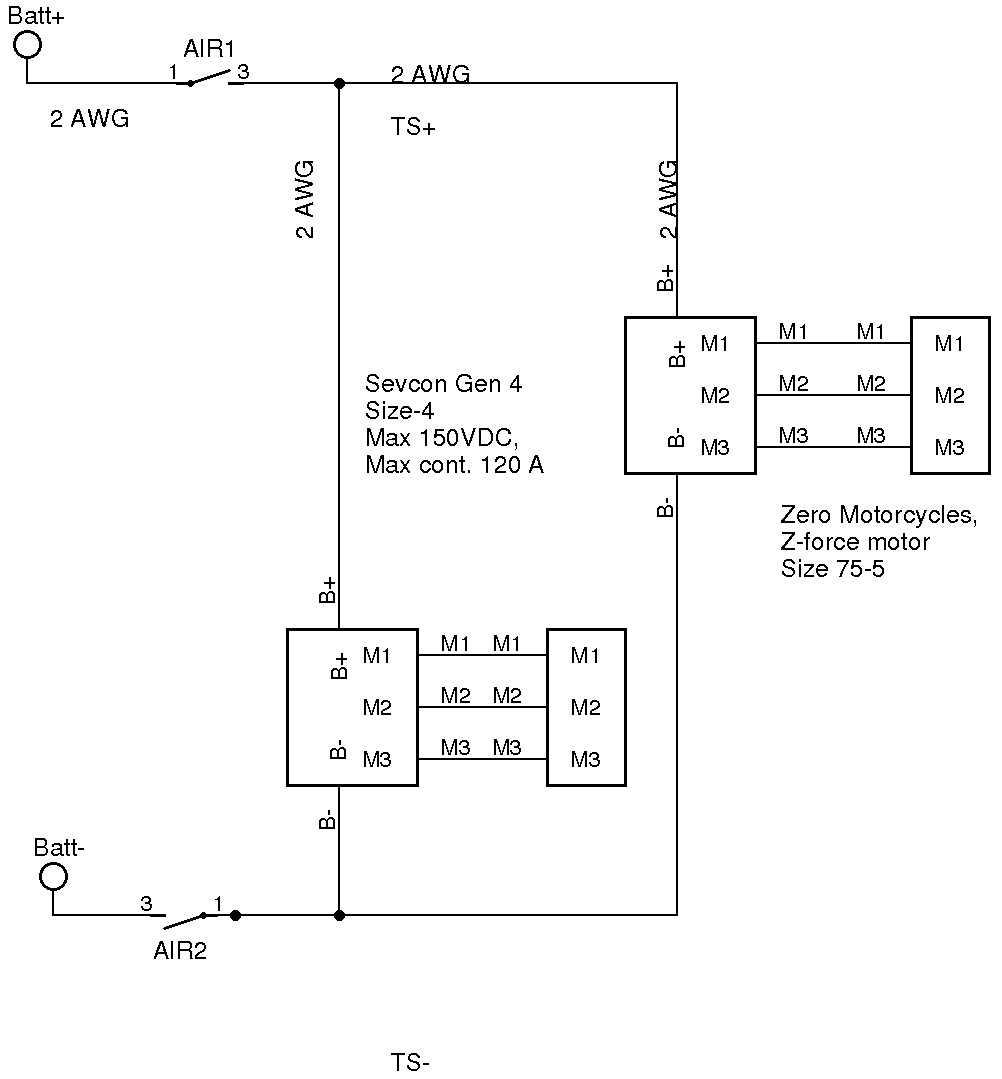
\includegraphics[width = 0.75 \textwidth]{motorcontroller}
                \caption{Schematic of the motor and motor controllers, in the tractive system}
                \label{mcschem}
            \end{figure}

            %Referred from section \ref{accumwiring} (AMS wiring), \ref{motorswiring}

            Both motors will follow the configuration in Figure \ref{mcschem}, parallel to the TS system. All high current wire gauges will be 2 AWG: the wire before the split to the motor controller, the wire to each controller, and the wire to each motor. There is a 175A fuse located before the AIRs, which is smaller than the ampacity of 2 AWG wire according to appendix section \ref{AWGchart}.
            %should i go into what we expect the motors to pull?

        \subsubsection{Position in Car}

            The motor controllers are located in the rear of the car, mounted to the main hoop bracing via steel brackets. This configuration is shown in Figures \ref{mcsideview}, \ref{mciso}, and \ref{mcrearview}. The controllers are entirely contained within the envelope of the chassis such that in any rollover attitude, the controllers will not make contact with the ground. \hlr{The covers for the motor controllers are still being designed. They will protect the motor controllers from being touched and rain.}

            \begin{figure}[H]
                \centering
                \includegraphics[width = 0.6 \textwidth]{motorcontroller_sideview}
                \caption{Side view of the motor controllers, mounted}
                \label{mcsideview}
            \end{figure}

            \begin{figure}[H]
                \centering
                \includegraphics[width = 0.6 \textwidth]{motorcontroller_isoview}
                \caption{Isometric view of the motor controllers, mounted}
                \label{mciso}
            \end{figure}

            \begin{figure}[H]
                \centering
                \includegraphics[width = 0.6 \textwidth]{motorcontroller_rearview}
                \caption{Rear view of the motor controllers, mounted}
                \label{mcrearview}
            \end{figure}

    \subsection{Motor Controller 2} \label{MC2}

        The second motor controller used will be exactly identical to that described in the section \ref{MC1}. Its wiring is shown in Figure \ref{mcschem}.

\newpage

\section{Motors} \label{Motors}

    \subsection{Motor 1} \label{M1}

        \subsubsection{Description, Type, Operating Parameters}

            %Describe the motor used, provide table with main parameters like resulting voltages->minimum, maximum, nominal, currents, resulting motor power, use figures to show important characteristics.

            \begin{figure}[H]
                \centering
                \includegraphics[width = 0.5 \textwidth]{motor_isorear}
                \caption{Isometric view of the 75-5 Z-force motor}
                \label{motoriso}
            \end{figure}

            We will use Zero Motorcycles Z-force BLDC Motors (75-5 Size), shown in Figure \ref{motoriso}. They are 3-phase DC brushless motors, compatible with the motor controllers used and described in Section \ref{MC1}.

            \begin{table}[H]
            \centering
            \begin{tabular}{|l|l|}
            \hline
            Motor Manufacturer and Type: & \begin{tabular}[c]{@{}l@{}}Zero Motorcycles,\\ Model \# 30-0534\end{tabular} \\ \hline
            Motor principle & DC Brushless \\ \hline
            Maximum continuous power & 24.9 kW per motor \\ \hline
            Peak Power & 41.8 kW per motor\\ \hline
            Input voltage & 99.6V \\ \hline
            Nominal current & 250 A \\ \hline
            Peak current & 420 A \\ \hline
            Maximum torque & 85 ft-lb \\ \hline
            Nominal torque & 75 ft-lb \\ \hline
            Cooling method & Air \\ \hline
            \end{tabular}
            \caption{General motor data}
            \label{motortable}
            \end{table}


            %plot of power vs rpm, including a line for nom and max power
            %plot of torque vs rpm, including a line for nom and max torque
            %so...we're missing maximum

            \begin{figure}[H]
                \centering
                \includegraphics[width = 0.75 \textwidth]{fx-motor-power-torque}
                \caption{}
                \label{motorplot}
            \end{figure}

            The motor's maximum power and torque were measured by Zero Motorcycles and graphed in figure \ref{motorplot}. The accumulator used in the motorcycle for this motor has a lower operating voltage. \hlr{Assuming a linear relationship between voltage and current, and a linear relationship between current and torque}, approximately 85-ft-lbs of peak torque in the flat linear range is expected.

        \subsubsection{Wiring, Cables, Current Calculations, Connectors} \label{motorswiring}

            %wiring, schematics, calcs for currents and voltages and show data regarding the cables and connectors

            The wiring from the motor controllers will simply connect the M1, M2 and M3 outputs of the motor controllers to the motors' inputs. Refer to Figure \ref{mcschem} for the schematic of motor 1 and motor 2. All power wires will be 2 AWG, described in Section \ref{mcwire}.
            \hlr{There will be a housing around the motor controllers so the TS connections cannot be touched, but it isn't currently designed. ESF will be updated when it is.}

        \subsubsection{Position in Car}

            The motors will be located behind the driver and accumulator, as shown in figures \ref{motormountrear}- \ref{motormountiso}. It is mounted to a steel face plate and a single stage chain transmission.

            \begin{figure}[H]
                \centering
                \includegraphics[width = 0.6 \textwidth]{motormount_sideview}
                \caption{Side view of the motor mount}
                \label{motormountside}
            \end{figure}

            \begin{figure}[H]
                \centering
                \includegraphics[width = 0.6 \textwidth]{motormount_rearview}
                \caption{Rear view of the motor mount}
                \label{motormountrear}
            \end{figure}

            \begin{figure}[H]
                \centering
                \includegraphics[width = 0.6 \textwidth]{motormount_isoview}
                \caption{Isometric view of the motor mount}
                \label{motormountiso}
            \end{figure}

    \subsection{Motor 2} \label{M2}

        The second motor used will be exactly identical to that described in section \ref{M1} and its wiring is also shown in figure \ref{mcschem}.

\newpage

\section{Torque Encoder} \label{TorqueEncoder}

    \subsection{Description/Additional Circuitry}

        Two rotary potentiometers are mechanically housed in one unit from Active Sensors (P/N MHR5621) and mounted to the rotating shaft of the throttle pedal assembly. The use of a single housing eliminates concerns regarding mechanical backlash and misalignment. Each output from the potentiometers will go to a CAN connected ATmega16M1, which will compare the two outputs and send a message via CAN bus to the motor controllers with the requested torque.

        \begin{table}[H]
        \centering
        \begin{tabular}{|l|l|}
        \hline
        Torque encoder manufacturer and type: & MHR5621 from Active Sensors \\ \hline
        Torque encoder principle & Potentiometer \\ \hline
        Supply voltage & 5V \\ \hline
        Maximum supply current & 15 mA \\ \hline
        Operating temperature & -55 to 150 \degree C \\ \hline
        Used output & 0-5V \\ \hline
        \end{tabular}
        \caption{Torque Encoder data}
        \label{encoder}
        \end{table}

        \begin{figure}[H]
            \centering
            \includegraphics{CANtorque}
            \caption{Schematic for the CAN node on the torque encoders}
            \label{torqueencoders}
        \end{figure}

    \subsection{Torque Encoder Plausibility Check}

        %This is describing the BSPD, I think they are asking about comparing the two potentiometer values. The Active Sensors encoder is ONE PHYSICAL UNIT with two potentiometers built-in.

        Two potentiometers are mounted on the torque pedal. A CAN node probes the voltage dividers. The ATmega will compare the two independent voltages and will only send non-zero torque commands if the sensors read a voltage within 10\% of each other. If a short circuit or wiring failure with either potentiometer occurs, the input will be outside the normal operating range, and the motor controllers will not be sent torque requests. The node will log the error in the CAN bus.\\

        There will also be a Pegasus Brake light pressure switch (part number 3601, recommended by Formula Hybrid) on the brakes, wired to a CAN node with 22 gauge wire. If the pressure switch indicates actuation of the brake and the potentiometers measure more than 25\% pedal travel, the power to the motors will be completely stopped until the torque pedal indicates less than 5\% pedal travel.

    \subsection{Wiring}

        %describe wiring, show schematics, data on cables and connectors

        \begin{figure}[H]
            \centering
            \includegraphics{torquebrakecheck}
            \caption{Schematic of the torque encoder plausibility check}
            \label{braketorque}
        \end{figure}

        Two potentiometers are wired with their output to the CAN analog input pins. The potentiometers are given separate power lines of 5V, parallel, to the supply power of the CAN node itself. The brake switch is positioned to trip at a level of hard braking, and when triggered will deliver 5V to a CAN input pin. The CAN node is wired to send and receive messages to the other nodes.

    \subsection{Position in Car/Mechanical Fastening/Mechanical Connection}

        %mechanical connection of the sensors

        The torque encoder is bolted to the accelerator pedal assembly with 4x ¼”-20 bolts. The bolts are safety-wired to prevent loosening. The torque encoder is manufactured with a D-shaft. This is rotationally fixed to the accelerator pedal axle by a 4-40 set screw. The set screw is bonded with Loctite Purple to prevent loosening. This allows the torque encoder to measure the angular position of the accelerator pedal axle. The accelerator pedal axle is prevented from moving axially by retaining rings. The mounting of the torque encoder does not affect the relative plausibility check. The sensor used contains two independent encoders, each measuring the position of the single shaft.

        \begin{figure}[H]
            \centering
            \includegraphics[width = 0.5 \textwidth]{torqueencoder}
            \caption{Mechanical fastening and connection to the throttle pedal. Note that the torque encoders are two encoders housed in one package}
            \label{torquefront}
        \end{figure}

        \begin{figure}[H]
            \centering
            \includegraphics[width = 0.7 \textwidth]{torqueside}
            \caption{Side view of how the torque encoder connects to the pedal and measures the throttle}
            \label{torqside}
        \end{figure}

        \begin{figure}[H]
            \centering
            \includegraphics[width = 0.7 \textwidth]{torquefullcar}
            \caption{Overall view of the torque encoder's position in the car, top down view}
            \label{torquetopdown}
        \end{figure}

\newpage

\section{Additional LV-parts Interfering with the Tractive System}

    \subsection{LV Part 1: DC-DC converter}

        \subsubsection{Description}

            \hlr{The GLV system will be powered via a DC/DC converter which will convert the 100V system to a 13.5V low voltage system. Before the DC-DC converter, there is a fuse for the GLV system as a whole, with a rating of 4A.}

        \subsubsection{Wiring, Cables}

            \begin{figure}[H]
                \centering
                \includegraphics{CANnodepower}
                \caption{DC-DC converter and its attachment to the GLV and then CAN node systems through a module}
                \label{dc-dcglv}
            \end{figure}

            %need wire gauges
            \hlr{Its output will be fused to 4A, and then used for the GLV system as 13.5V. After the two emergency shutdown buttons, the system is fused in parallel with two 2A fuses (the system voltage will be fused to 2A and the shutdown system will be fused to 2A). The GLV system voltage will be split in parallel again and then regulated to 5V for the sake of the CAN ATmega. All of these wires, past the DC-DC converter, will be 20 AWG.}

        \subsubsection{Position in Car}

            The DC-DC converter will be located within the accumulator, so the output leads will go out of the accumulator. Figure \ref{dcdc_cad} shows the CAD model of the DC-DC converter, \hlr{which will be located in the side panel housing described in figure} \ref{cpanel1}.

            \begin{figure}[H]
                \centering
                \includegraphics[width = 0.5 \textwidth]{GLV_DCDC}
                \caption{CAD model of the DC-DC converter for the GLV system}
                \label{dcdc_cad}
            \end{figure}

    \subsection{LV Part 2: Dashboard Node}

        \subsubsection{Description}

            The Dashboard node will have a variety of tasks. It will act as the Control Panel interface (for displaying information to the driver and receiving data from the driver), Emergency Button sensor, \hlr{AMS light, IMD light and start button}.\\

            The control panel interface is used for debugging. \hlr{The CAN system has nodes all over circuits in the car.} If the CAN system is still live (when an E-stop hasn't been pushed and the GLV master switch is on), then this CAN node will alert the driver.\\

            The node is connected to a linear potentiometer on the steering rack. The potentiometer's value corresponds to the steering angle, so the CAN node can transmit the information on all of the turns. This node is used for driver training, practice, and team information in later years. If time permits, this data can be used to help in the development of \hlr{torque vectoring.}\\

        \subsubsection{Wiring, cables}

            \begin{figure}[H]
                \centering
                \includegraphics[width = 0.8 \textwidth]{CANdashboard}
                \caption{Dashboard node schematic}
                \label{dashschem}
            \end{figure}

            The dashboard node is wired to have the \hlr{E-stops as input} and the control panel interface (the LED) as an output. It listens to all CAN messages around the car. The interfacing LED will notify the driver of anything deemed important, such as the AMS detecting the temperature of the accumulator cells was getting too high. Therefore, the dashboard's interfacing light will mostly be telling the driver why the shutdown system shut down through a series of flashes. Only if one of the E-stops are pressed will the CAN system shut down and therefore the interfacing light will not tell the driver what has happened to the shutdown circuit.

        \subsubsection{Position in Car}

            The dashboard node will be located behind the dashboard, and connecting to certain switches and lights on the dashboard. The dashboard CAD render can be shown in Figure \ref{dashboard}.

            \begin{figure}[H]
            \centering
            \includegraphics[width = 0.7 \textwidth]{Dashboard}
            \caption{Render of the Dashboard, the location of the dashboard node. }
            \label{dashboard}
            \end{figure}

    \subsection{LV Part 3: Side Panel Node} \label{imdnode}

        \subsubsection{Description}

            The node located next to the IMD and ready to drive sound monitors the IMD's output and will activate the ready to drive sound when the car is in ready mode. It will receive input from behind each of the two side e-stops, so if one is pushed, the CAN system knows and can tell the driver the reason for shutdown circuit shutdown. It will also be connected to the rest of the CAN system around the car and listen to CAN messages for anomalies. If the Watchdog node receives a CAN error message that indicates danger to the driver or the vehicle it will open the watchdog switch in the shutdown circuit. This will be useful for maintaining the health of the motor controllers.

        \subsubsection{Wiring, Cables}

            % \begin{figure}[H]
            % \centering
            % \includegraphics[width = 0.8 \textwidth]{IMDandCANschem}
            % \caption{Schematic for the node on the ready to drive sound, watchdog, and side e-stops and IMD}
            % \label{panelnode}
            % \end{figure}

            \begin{sidewaysfigure}[p]
            \includegraphics[width=\textheight]{Panel-Board}
            \caption{\hlr{Side Panel node wiring. The PCB's schematic, shown here, includes TS wiring going to the TSMPs, IMD and R2D sound.}}
            \label{panelnode}
            \end{sidewaysfigure}

            As shown in Figure \ref{panelnode}, both the IMD and the ready to drive sound relay are wired to the CAN node located in the \hlr{side panel housing}.\\

            The CAN node is wired to the \hlr{third} pole of the IMD relay, \hlr{and the node will always read low }until the pole is no longer pulled because the IMD's output is low and the IMD has found a ground fault. \hlr{There is a pull up resistor and the pole, in its disconnected state the can input will read 5V instead.}\\

            As an output, the CAN node is also wired to a relay's coil controlling a switch in the tractive system parallel to the motors. When the CAN system knows it's in ready to drive mode, it'll send the message to send 5V to this coil, therefore closing the switch that will give the ready to drive sound buzzer power to make noise.\\

            Also an output of the CAN node is the watchdog relay that controls a switch in the shutdown circuit. As watchdog of the CAN system, if a CAN node goes silent and suddenly stops messaging the rest of the system, this node will take notice and stop sending 5V to this coil, making it open the shutdown circuit. This will protect the motor controllers and offer redundancy for the rest of the shutdown circuit.

        \subsubsection{Position in Car}

            The \hlr{side panel} node will be contained in the enclosure shown in Figure \ref{cpanel2}.

\newpage

\section{Overall Grounding Concept}

    \subsection{Description of the Grounding Concept}

        %Describe how you intend to achieve the resistances between components at the required levels as defined in EV 4.3

        The chassis is used as GLV ground. This ground is established at the panel mount holding many of the shutdown components \hlr{the TSMPs, GLV DC-DC converter and GLV battery}. All mechanical systems in the vehicle, such as the accumulator, drivers seat, and pedal box, achieve low resistance to ground because they are either welded directly to the chassis, or fastened using uncoated, conductive metal fasteners. Electrical systems that are satellite to the main panel mount that need to establish a connection to ground for sense purposes are grounded to the chassis using ring terminals. Ring terminals can be included in the bolt stack up of mechanical systems to ensure a secure connection to ground that is positively retained with a lock nut.


    \subsection{Grounding Measurements}

        %Describe the measurements you'll take to make sure EV4.3 is achieved
        The conductive components within 100mm of the tractive system or a GLV component will be measured with a multimeter \hlr{using in a 4pt technique}to have less than 300 m\ohm resistance to ground. All fastened mechanical systems will be measured for a ground connection individually and exhaustively. Continuity will be checked during manufacture and assembly before the GLV system is in place.\\

        \hlr{There will not be any carbon fiber on the vehicle.}

\newpage

\section{Firewall}

    \subsection{Firewall 1}

        \subsubsection{Description/Materials}

            %Show how the low resistance Control System ground connection is achieved.
            The firewall is constructed of two layers. The layer facing the tractive system is \hlr{1.5} mm Aluminum sheet metal, with a chamfered edge. The second layer facing the cockpit is 1/8 in. Flame-Retardant Multipurpose Garolite (G-10/FR4). The assembly is fastened together using sheet metal rivets. The chassis has welded sheet metal tabs that fasten to the firewall with bolts and lock nuts. Because the firewall is fastened to the chassis using conductive fasteners it is connected to GLV ground.

            All high voltage and high temperature systems are contained in the rear of the vehicle, so only one firewall will be used. There are GLV systems in the dashboard and pedal box so a small grommeted hole will be made in the firewall for GLV wiring.

            \begin{figure}[H]
                \centering
                \includegraphics[width = 0.6 \textwidth]{ExplodedView}
                \caption{Exploded view of the firewall}
                \label{explodedfirewall}
            \end{figure}

        \subsubsection{Position in Car}

            The firewall is located between the driver and the accumulator, to protect the driver from the TS. Figure \ref{firewallposition} shows the position with the driver seat removed for visual aid. The seat will go in the gap between the wheel and the firewall, facing away from the firewall. The top corner of the extruded part of the firewall is chamfered in order to protect the driver and will also be covered with padding.

            \begin{figure}[H]
                \centering
                \includegraphics[width = 0.8 \textwidth]{FirewallFullCarView}
                \caption{CAD render of the firewall's position in the car}
                \label{firewallposition}
            \end{figure}

    \subsection{Firewall 2}
        There is only one firewall in the vehicle.

\newpage

\section{Appendix}
\section*{11.2.1.1 Shutdown Switches} \label{shutdownappendix}

\href{http://products.eao.com/index.php?IdTreeGroup=2344&IdProduct=48667&lang=en}{Cockpit E-Stop Button Datasheet here}.

\href{http://products.eao.com/index.php?IdTreeGroup=2344&IdProduct=48533&lang=en}{Right and Left E-Stop Buttons Datasheet here}.

\href{http://www.amazon.com/Volt-Battery-Disconnect-Kill-Switch/dp/B007O0BBFM}{Tractive System and GLV System Master Switches, product link here, no datasheet available}.

\href{http://www.mouser.com/pdfdocs/9876510101.PDF}{Main connector to the accumulator, also an interlock, datasheet here}.

See section \ref{bspdappendix} for the AMS and BSPD relays.
%Main connector here
See section \ref{IMDRepTime} for the IMD relay.
See section \ref{hvdappendix} for the HVD.
See section \ref{inertiaappendix} for the inertia switch.

\section*{11.2.2 IMD datasheet} \label{IMDRepTime}
\begin{figure}[H]
    \centering
    \includegraphics[width=0.45 \textheight]{IMD_datasheet_snip}
    \caption{Response value information from IMD datasheet}
    \label{IMDresponsetime}
\end{figure}

\href{http://www.bender.org/documents/IR155-10_datasheet_NAE1012821.pdf}{Full IMD Datasheet here}.

\href{http://www.automationdirect.com/static/specs/78relays.pdf}{IMD 4PDT Relay Datasheet Here}. Referred from section \ref{shutdownappendix}.

\href{http://www.littelfuse.com/~/media/electronics/datasheets/fuses/littelfuse_fuse_251_253_datasheet.pdf.pdf}{Fuse that protects the IMD, 251/253 series (1A)}

\section*{11.2.3 Inertia switch} \label{inertiaappendix}

\href{http://www.sensata.com/download/resettable-crash.pdf}{Sensata Resettable Crash sensor datasheet here}. Referred from section \ref{shutdownappendix}.

\section*{11.2.4 Brake Plausibility Device} \label{bspdappendix}

\href{http://www.te.com/commerce/DocumentDelivery/DDEController?Action=srchrtrv&DocNm=PB&DocType=DS&DocLang=English}{BSPD relay}. Reffered from section \ref{shutdownappendix} (shutdown system), section \ref{r2dappendix} (ready to drive sound), section \ref{prechargeappendix} (precharge system), and section \ref{amsappendix} (AMS).

See section \ref{torqueappendix} for the brake sensor's datasheet.

\section*{11.2.7 Tractive System Active Light}

\href{http://www.mouser.com/ds/2/281/mdc_ruw15-217876.pdf}{DC-DC converter for the TSAL datasheet}.

\href{https://www.superbrightleds.com/moreinfo/oval-marker-lamps/oval-led-truck-trailer-light-with-reflectorized-lens-4in-led-marker-clearance-light-with-4-leds/580/#/tab/Specifications}{Product information for the TSAL}.

\href{http://www.onsemi.com/pub_link/Collateral/1N5333B-D.PDF}{Zener with 56V breakdown, for activating the TSAL}.

\section*{11.2.8.2 Tractive System Measuring Points} \label{tsmpappendix}

\href{https://www.gossenmetrawatt.com/resources/tt/hit27/db_gb.pdf}{Expected multimeter to measure the TS voltage, datasheet here}.

\href{http://www.mouser.com/ds/2/427/cmfind-239942.pdf}{\hlr{5K, 1.5W resistors for the TSMP datasheet here}.}

\href{http://www.mouser.com/ds/2/159/D72930_02_10_06-21562.pdf}{Red and Black TSMP 4mm banana jack datasheet here}.

\section*{11.2.9 Precharge System}
\label{prechargeappendix}

Please see section \ref{bspdappendix} for the relay used for the keyswitch's power.

\section*{11.2.10 Discharge system} \label{dischargeappendix}

\begin{figure}[H]
    \centering
    \includegraphics[width = 0.8 \textwidth]{Dischargeres}
    \caption{Power overload graph of the 100W discharge resistor}
    \label{disres}
\end{figure}

\href{http://www.farnell.com/datasheets/1498243.pdf}{\hlr{Discharge resistor datasheet here}.}

\href{http://cotorelay.com/product/5500-series-high-voltage-reed-relays/}{\hlr{Discharge relay datasheet here.}}

Referred from section \ref{dischargesection}

\section*{11.2.11 HVD } \label{hvdappendix}

\href{http://www.andersonpower.com/_global-assets/downloads/pdf/ds-smart.pdf}{HVD Anderson connector datasheet here}. Referred from section \ref{shutdownappendix}.

\section*{11.2.12 Ready to Drive Sound} \label{r2dappendix}

\href{http://www.mouser.com/ds/2/252/SC648ANR-63353.pdf}{\hlr{Ready to drive sound buzzer datasheet}}.

Please refer to section \ref{bspdappendix} for the relay of the ready to drive sound.

\section*{11.3.1.2 Cell Description}
We are working with Nissan to allow us to use their datasheet for the modules.

\section*{11.3.1.4 Cell Temperature Monitoring}

\href{http://media.digikey.com/PDF/Data\%20Sheets/Ametherm\%20PDFs/PANR\%20103395-408.pdf}{Thermistors measuring cell temperature datasheet}.

\section*{11.3.1.5 Accumulator Monitoring System}  \label{amsappendix}

\begin{figure}
    \centering
    \includegraphics[width = 1 \textwidth]{BMS_Schem}
    \caption{Schematic of one of the accumulator monitoring boards}
    \label{amsschem}
\end{figure}

% end{sidewaysfigure}
Please see figure \ref{amsschem} for the schematic of the AMS boards. Referred from section \ref{bms}. The AMS looks at the voltage of each cell by having differential amplifiers between two cells and get a relative voltage. This relative voltage for each cell is then put through an optocoupler, which then connects a power resistor and transistor to shunt the cell when necessary. There is an isolated CAN node attached to the board so it can communicate to the rest of the shutdown system and activate a relay to open the shutdown circuit when necessary. The BMS connects to the cell-top boards, shown in figure \ref{celltopschem}.

Please see section \ref{bspdappendix} for the AMS relay.

\section*{11.3.1.8 Accumulator Insulation Relays}

\href{http://www.rec-bms.com/datasheet/Technical_datasheet_Kilovac.pdf}{Accumulator Insulation Relay datasheets here}.

\section*{11.3.1.9 Fusing} \label{fusingappendix}

Referred from section \ref{fusing}.

\begin{figure}[H]
    \centering
    \includegraphics{TSmainratings}
    \caption{\hlr{Ratings for the Bussman LPJ series 175A main TS fuse}}
    \label{mainTSfuseratings}
\end{figure}

\begin{figure}[H]
    \centering
    \includegraphics[width = 0.7 \textwidth]{TSfuseT-Agraph}
    \caption{\hlr{Time-current curve for Bussman LPJ series 175 A main TS fuse}}
    \label{mainTSfusecurve}
\end{figure}

All information found from the datasheet of:
\href{http://www.allfuses.com/media/documents/Bussmann\%20LPJ\%20(70-600A).pdf}{Full Bussman Fuse LPJ 175A datasheet here}.

%no longer have msd fuses
% \href{http://www.stormcopper.com/design/Ampacity-Quick-Chart.htm}{StormCopper Busbar Ampacity Chart}.
\begin{figure}[H]
    \centering
    \includegraphics[width = 0.6 \textwidth]{Keyswitchratings}
    \caption{\hlr{Ratings taken from the A15QS, 7A Keyswitch fuse}}
    \label{keyswitchratings}
\end{figure}

\begin{figure}
    \centering
    \includegraphics[width = 0.7 \textwidth]{Keyswitchmeltingtime}
    \caption{\hlr{Time-Current curve for A15QS, 7A Keyswitch fuse}}
    \label{keyswitchcurve}
\end{figure}

All information found from the datasheet of:
\href{http://www.allfuses.com/media/documents/Ferraz\%20A15QS.pdf}{\hlr{Keyswitch Fuse datasheet, Semiconductor AC A15QS}}.

\begin{figure}[H]
    \centering
    \includegraphics[width = 0.6 \textwidth]{TSsmallratings}
    \caption{\hlr{251/253 series, 1A TS low current fuse}}
    \label{tssmallratings}
\end{figure}

\begin{figure}[H]
    \centering
    \includegraphics[width = 0.6 \textwidth]{TSsmallmeltingtime}
    \caption{\hlr{Time-Current curve for 251/253 series 1A TS low current fuse}}
    \label{TSsmallcurve}
\end{figure}

All information found from the datasheet of:
\href{http://www.littelfuse.com/~/media/electronics/datasheets/fuses/littelfuse_fuse_251_253_datasheet.pdf.pdf}{\hlr{TS to IMD, TSMP and Lights DC-DC converter, 1A 251/253 Series}}

\begin{figure}[H]
    \centering
    \includegraphics[width = 0.6 \textwidth]{GLVmainratings}
    \caption{\hlr{SPF Series, 4A Main GLV fuse}}
    \label{glvmainratings}
\end{figure}

\begin{figure}[H]
    \centering
    \includegraphics[width = 0.6 \textwidth]{glvmainmeltingtime}
    \caption{\hlr{Time-current curve for SPF series 4A GLV main fuse}}
    \label{Glvmaincurve}
\end{figure}

\hlr{All information found from the datasheet of: }
\href{http://www.allfuses.com/media/documents/Littelfuse_Fuse_Solar_SPF_Datasheet.pdf}{GLV main fuse, 4A SPF type}.

\begin{figure}[H]
    \centering
    \includegraphics[width = 0.6 \textwidth]{AMSfuseratings}
    \caption{\hlr{Ratings for C1Q 3A Cell series to AMS fuse}}
    \label{amsfuseratings}
\end{figure}

\begin{figure}[H]
    \centering
    \includegraphics[width = 0.6 \textwidth]{amsfuseapprovals}
    \caption{\hlr{Approved Ratings of C1Q series 3A Cell to AMS fuse}}
    \label{amsfuseapproval}
\end{figure}

\begin{figure}[H]
    \centering
    \includegraphics[width = 0.6 \textwidth]{amsfusecurve}
    \caption{\hlr{Time-current curve for C1Q series, 3A Cell to AMS fuse}}
    \label{amsfusecurve}
\end{figure}

\hlr{All information found from the datasheet of: }
\href{http://belfuse.com/pdfs/C1Q.pdf}{Cell to AMS fuse, C1Q type}.

\begin{figure}[H]
    \centering
    \includegraphics[width = 0.6 \textwidth]{shutdownfuseratings}
    \caption{\hlr{Ratings for MINI series, 2A Shutdown circuit and GLV 12V fuses}}
    \label{shutdownfuseratings}
\end{figure}

\begin{figure}[H]
    \centering
    \includegraphics[width = 0.6 \textwidth]{shutdownfusecurve}
    \caption{\hlr{Time-current curve for MINI series, 2A Shutdown and GLV 12V fuses}}
    \label{shutdownfusecurve}
\end{figure}

\hlr{All information found from the datasheet of: }
\href{http://www.littelfuse.com/~/media/automotive/datasheets/fuses/automotive-fuses/littelfuse_automotive_blade_fuse_mini_32v.pdf}{GLV 12V power and Shutdown circuit fuses, MINI series 2A}

\begin{figure}
    \centering
    \includegraphics[width = 1 \textwidth]{WireGaugeChart}
    \caption{Power Stream Wire Gauge Chart Reference. Reffered from section \ref{fusing}}
    \label{AWGchart}
\end{figure}

\section*{11.3.1.10 Charging}

\begin{figure}[H]
    \centering
    \includegraphics[width = 0.8 \textwidth]{chargerdata}
    \caption{Important data of the 96V charger, from datasheet}
    \label{chargerdatasheet}
\end{figure}

\href{http://delta-q.com/wp-content/uploads/2015/12/Delta-Q_QuiQ1000_BatteryCharger_Specifications.pdf}{Delta Q Technologies 96VDC charger datasheet}.

\section*{11.5.1 Motor Controller}

\href{http://www.sevcon.com/media/2461/Gen4\%20Aug\%202013\%20web.pdf}{Motor controller Sevcon Gen 4 Size 4 with battery voltage 96-120V datasheet here}.

\href{http://www.thunderstruck-ev.com/Manuals/Gen4_Product_Manual_V3.0.pdf}{Sevcon Gen4 Product Manual}

\section*{11.7 Torque Encoder} \label{torqueappendix}

\href{https://www.pegasusautoracing.com/2015/086.pdf}{Brake light switch datasheet here, part number 3601}. Reffered from section \ref{bspdappendix}.

\begin{figure}[H]
    \centering
    \includegraphics[width = 0.6 \textwidth]{activesensorsnip}
    \caption{Important parameters of the MHR5621 Active Sensors Torque Encoder}
    \label{torquesnip}
\end{figure}

\href{http://www.magni-tec.com/datasheet/WS-MHR5200.pdf}{MHR5621 Active Sensors Torque Encoder datasheet}.

\section*{11.8.1 LV Part 1: DC-DC converter}

\href{https://www.superbrightleds.com/moreinfo/bar-strip-accessories/12vdc-to-5vdc-voltage-converter-/1549/3652/#/tab/Specifications}{12V to 5V module datasheet here}.

%need sevcon dc-dc
\href{http://www.evdrives.com/product_p/vr-sevcon-7213.htm}{Sevcon DC-DC converter product information here}.

\section*{11.8.2 LV Part 2: Dashboard node}.

\href{http://www.atmel.com/images/8209s.pdf}{CAN node microcontroller (ATmega16M1) datasheet here}.

%A datasheet for motor controller one for example has to have the numbering 11.10.5
%Example appendix entry:
%11.2.2 – Bender IR155-3203 IMD ratings
%Referred from 5.1.1.
%Picture of a section
%Link to full datasheet
%I\par
\end{document}
